%%% aQGC %%%
\chapter{Interpretation with Effective Field Theory}
\label{chap:aQGC}

%\subsection{Introduction}

%The boson field self-interactions respect the $SU(2)\times U(1)_Y$ gauge invariance in the electroweak sector of the SM and serve as a very sensitive tool to search for the manifestations of physics beyond the SM.
%The VBS is one of the processes directly sensitive to the quartic-gauge coupling vertices of the SM.
%Variations of these vertices from the SM are known as anomalous quartic-gauge couplings (aQGC), and can arise from alterations of the electroweak or Higgs sector of the SM.

%The effect of such new physics introduced by aQGC can be realized using the effective field theory~\cite{degrande2013effective} and linearly parameterized by the effective Lagrangian as:
%\begin{equation*}
%  \mathcal{L}=\mathcal{L}_{sm}+\sum_{i}\frac{c_i}{\Lambda^{2}}\mathcal{L}_i+\sum_{n}\frac{f_n}{\Lambda^{4}}\mathcal{L}_n,
%\end{equation*}
%where $\mathcal{L}$ represents possible dim-6 and dim-8 operators and $c_i$ and $f_n$ are correspond their wilson coefficients. The $\Lambda$ represents the energy scale over which the new degrees of freedom are integrated out. 
%In this note, the name of Lagrangian term that contains the given operator is denoted by its wilson coefficient i.e. $L_{n} = \frac{f_{n}}{\Lambda^4} O_{n}$ is called as $f_{n}$.
%The odd-dimension operators violate lepton and baryon number conservation and are ignored.
%Both of dim-6 and dim-8 operators can contribute to the VBS processes through aTGC and aQGC, respectively,
%but due to the tight constraints of dim-6 operators from inclusive diboson measurements, only dim-8 operators are discussed in this note.

%The Eboli model~\cite{eboli2006p} is employed to describe the signals, which introduces twentyone new dim-8 operators satisfying the SM $SU(2)\times U(1)_Y$ symmetry. 
%These operators can be categorized by the types of the coupling; scalar types that contain just covariant derivatives of the Higgs field: $f_{S0}$, $f_{S1}$, $f_{S2}$, tensor types  that contain just field strengths: $f_{T0}$, ..., $f_{T9}$, and mixed operators that exhibit two covariant derivatives of the Higgs field and two field strengths: $f_{M0}$, ..., $f_{M7}$. 
%Table~\ref{tab:operators} shows the vertices that can be modified by the given operator. 
%The operators $f_{S0}$ and $f_{S2}$ are Hermitian conjugates, so they are treated as one single operator by setting both coefficients to be the same value.
%The semileptonic VBS is a golden channel that can test nineteen oeperators simultaneously, which has  $WW$, $WZ$, and $ZZ$ pairs in the final state.
%It is found via simulations that the tensor operators produce purely transversely polarized $W/Z$ bosons, while the scalar operators longitudinal bosons.
%In particular in the merged analysis, higher selection efficiency for the scalar operators is expected since the boosted boson tagger is optimized for the logitudinally-polarized bosons.

%\begin{table}[ht!]
%\begin{center}
%\resizebox{0.70\textwidth}{!}{

%\begin{tabular}{|c|c|c|c|c|c|c|c|c|c|}
%\hline & WWWW & WWZZ & ZZZZ & WWAZ & WWAA & ZZZA & ZZAA & ZAAA & AAAA \\
%\hline $\mathcal{L}_{S02}, \mathcal{L}_{S1}$ & $\mathrm{X}$ & $\mathrm{X}$ & $\mathrm{X}$ & %$\mathrm{O}$ & $\mathrm{O}$ & $\mathrm{O}$ & $\mathrm{O}$ & $\mathrm{O}$ & $\mathrm{O}$ \\
%\hline $\mathcal{L}_{M0}, \mathcal{L}_{M1}, \mathcal{L}_{M6}, \mathcal{L}_{M7}$ & $\mathrm{X}$ & %$\mathrm{X}$ & $\mathrm{X}$ & $\mathrm{X}$ & $\mathrm{X}$ & $\mathrm{X}$ & $\mathrm{X}$ & %$\mathrm{O}$ & $\mathrm{O}$ \\
%\hline $\mathcal{L}_{M2}, \mathcal{L}_{M3}, \mathcal{L}_{M4}, \mathcal{L}_{M5}$ & $\mathrm{O}$ & %$\mathrm{X}$ & $\mathrm{X}$ & $\mathrm{X}$ & $\mathrm{X}$ & $\mathrm{X}$ & $\mathrm{X}$ & %$\mathrm{O}$ & $\mathrm{O}$ \\
%\hline $\mathcal{L}_{T0}, \mathcal{L}_{T1}, \mathcal{L}_{T2}$ & $\mathrm{X}$ & $\mathrm{X}$ & %$\mathrm{X}$ & $\mathrm{X}$ & $\mathrm{X}$ & $\mathrm{X}$ & $\mathrm{X}$ & $\mathrm{X}$ & %$\mathrm{X}$ \\
%\hline $\mathcal{L}_{T5}, \mathcal{L}_{T6}, \mathcal{L}_{T7}$ & $\mathrm{O}$ & $\mathrm{X}$ & %$\mathrm{X}$ & $\mathrm{X}$ & $\mathrm{X}$ & $\mathrm{X}$ & $\mathrm{X}$ & $\mathrm{X}$ & %$\mathrm{X}$ \\
%\hline $\mathcal{L}_{T8}, \mathcal{L}_{T9}$ & $\mathrm{O}$ & $\mathrm{O}$ & $\mathrm{X}$ & $\mathrm{O}$ & $\mathrm{O}$ & $\mathrm{X}$ & $\mathrm{X}$ & $\mathrm{X}$ & $\mathrm{X}$ \\
%\hline
%\end{tabular}

%}
%\caption{Correspondences between wilson coefficients and vertices. $\mathrm{X}$ shows the existence of the vertex with the interaction by the operator.}
%\label{tab:operators}
%\end{center}
%\end{table}

As mentioned in Section~\ref{subsec:EFT}, aQGC interpretation is done via EFT lagrangian. 
The SM+EFT matrix element can be written as
\begin{equation}
   |A_{SM}+\frac{f_i}{\Lambda^4}A_i|=|A_{SM}^2|+\sum\limits_i \frac{f_i^2}{\Lambda^8}|A_{i}^2|+ \sum\limits_i 2 \frac{f_i}{\Lambda^4} \mathrm{Re}(A_{SM}^\star A_i) +\sum\limits_{i\neq j} \frac{f_i}{\Lambda^4} \frac{f_j}{\Lambda^4} \mathrm{Re}(A_i^\star A_j)
\end{equation}
where $|A_SM|^2$ is the SM matrix element, $|A_{i}^2|$ represents the pure-EFT matrix elements for the $f_{i}$ operator, $2 \mathrm{Re}(A_{SM}^\star A_i)$ is its corresponding interference term with the SM, and $\mathrm{Re}(A_i^\star A_j)$ is possible interference term between EFT operators $f_{i}$ and $f_{j}$. 
Theoretically, it cannot separate the effects of Wilson coefficients $f_i$ and the scale $\Lambda^4$, so the parameter of interest in this analysis is the ratio $\frac{f_i}{\Lambda^4}$. %Sometimes it is just called as $f_i$.
The pure-EFT term is scaled by the quadrature of $\frac{f_i}{\Lambda^4}$ and the interference term by $\frac{f_{i}}{\Lambda^4}$.
Sometimes they are called as the quadratic term and the linear term, respectively.


\subsection{Clipping method}
\label{subsec:clipping}
As the EFT violates unitarity at large energy scale, the clipping method, mentioned in section~\ref{subsec:EFT}, is used to preserve the unitarity at high center of mass energies. 
The EFT signal is set to zero at truth $m_{VV} > E_{clip}$, where the $E_{clip}$ is [1.5, 2, 3, 5, $\infty$]~TeV. 
%Figure~\ref{fig:clipped} shows how the $m_{VV}$ is shown at the low clipping energy.
The background samples, which is the all standard model predictions, are not clipped.
%5 points are chosen as recommended from the anomolous gauge couplings (aGC) taskforce.~\cite{ATL-COM-PHYS-2017-433} 
5 points are chosen so that we can compare the results with other channels or experiments.
The expected and observed limits are obtained with all 3 channels at each of the clipping points, and compared with the theoretical unitarity bound.

%Minori : need to replace the histograms
%\begin{figure}[ht]
%    \centering
%    	\subfigure[ FT0 ]{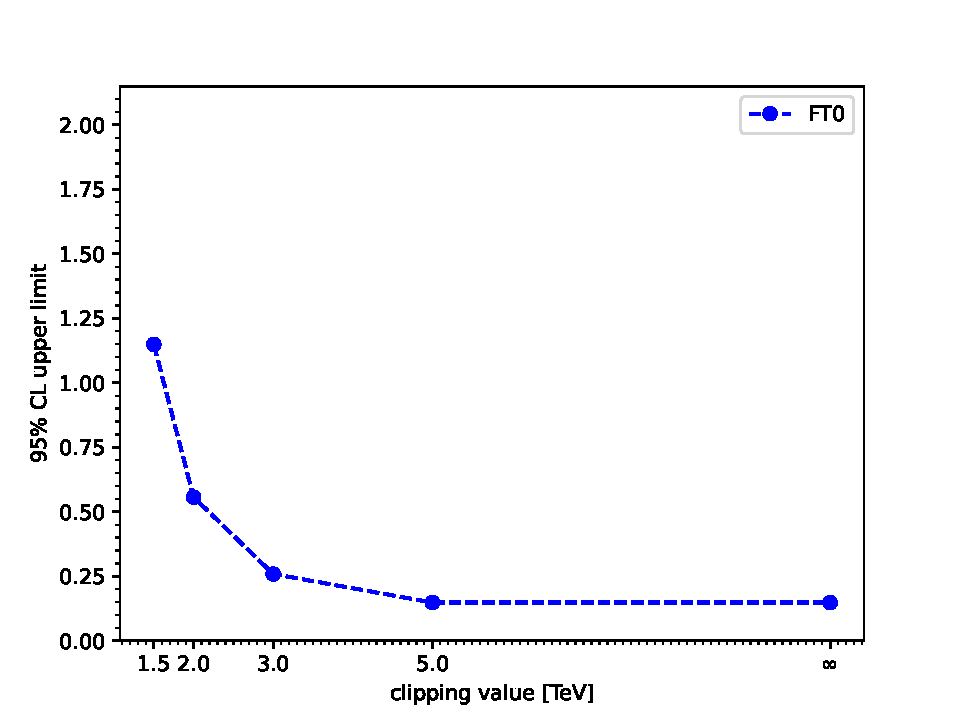
\includegraphics[width=0.32\textwidth]{figures/aQGC/ClippedFT0.pdf}}
%    	\subfigure[ FT1 ]{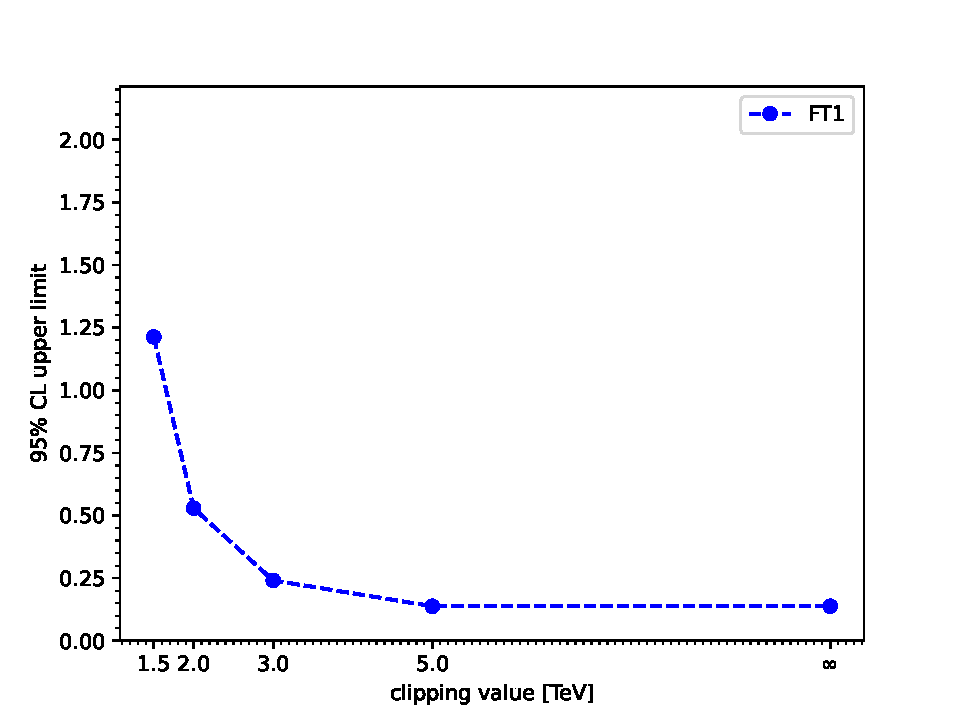
\includegraphics[width=0.32\textwidth]{figures/aQGC/ClippedFT1.pdf}}
%    	\subfigure[ FT2 ]{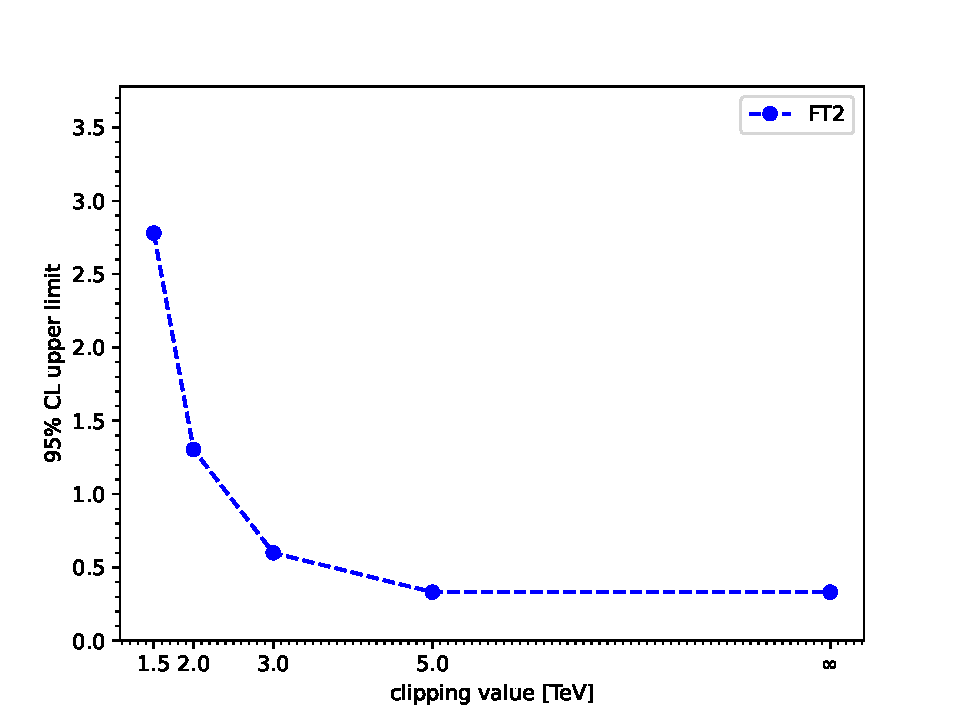
\includegraphics[width=0.32\textwidth]{figures/aQGC/ClippedFT2.pdf}}
%        \caption{Expected limits for 5 clipping points are shown for each coefficient FT0, FS02, and FM0.}
%        \label{fig:ClippedLimits}
%\end{figure}
%
%\begin{figure}[ht]
%    \centering
%    	\subfigure[ FT5 ]{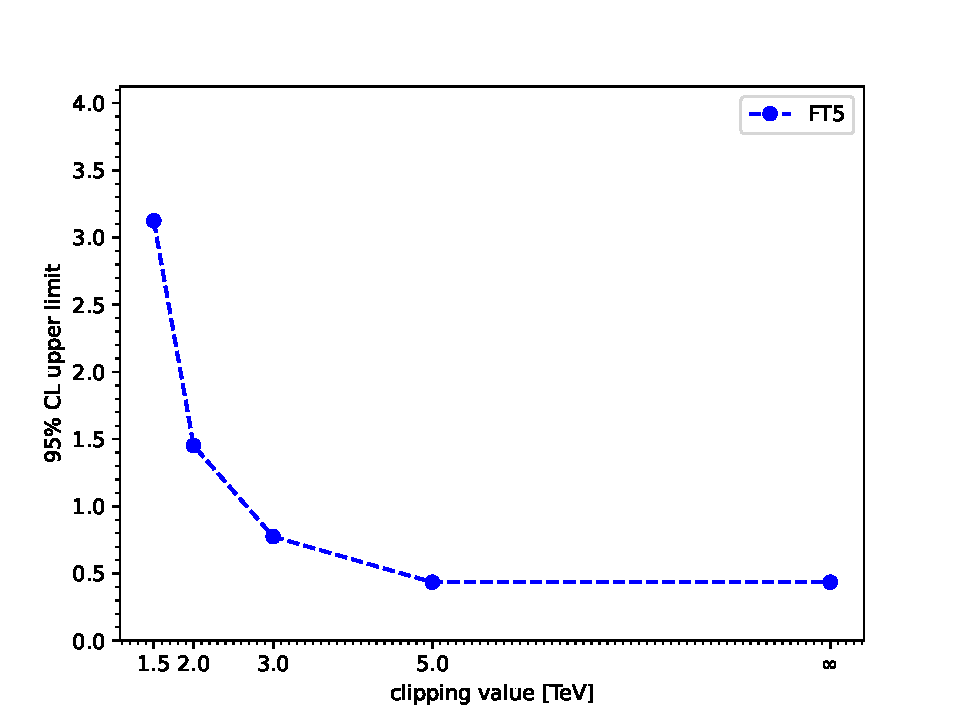
\includegraphics[width=0.32\textwidth]{figures/aQGC/ClippedFT5.pdf}}
%    	\subfigure[ FT6 ]{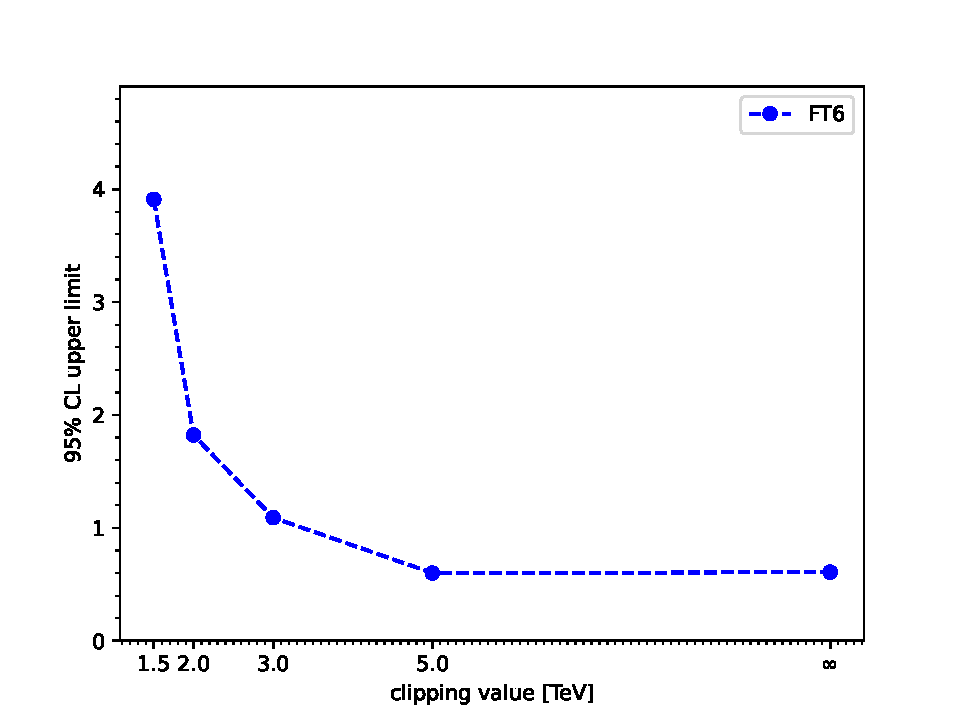
\includegraphics[width=0.32\textwidth]{figures/aQGC/ClippedFT6.pdf}}
%    	\subfigure[ FT7 ]{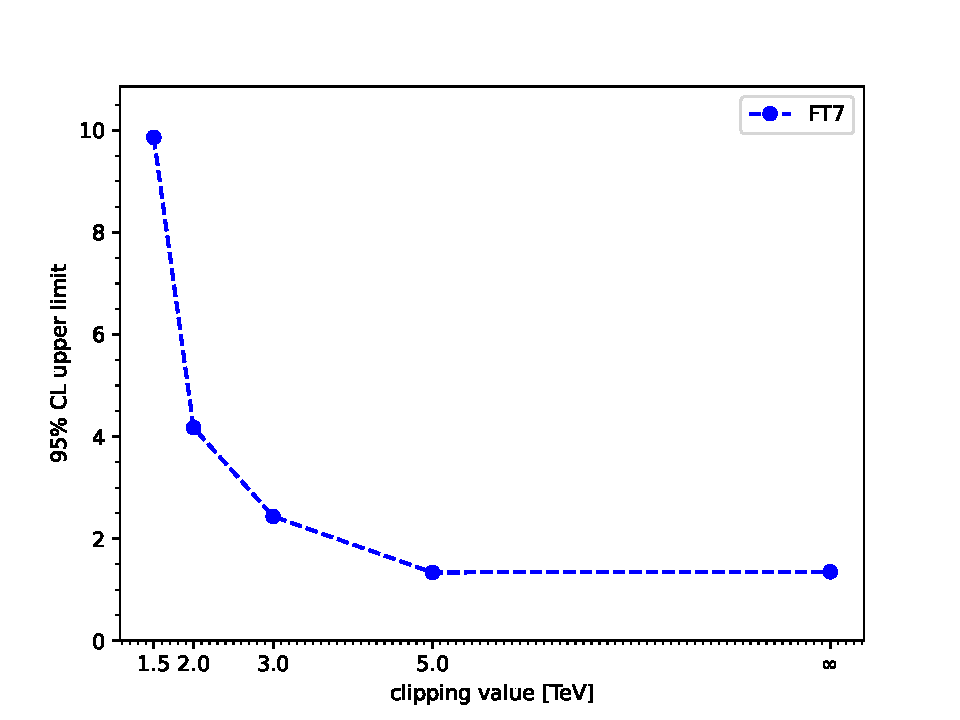
\includegraphics[width=0.32\textwidth]{figures/aQGC/ClippedFT7.pdf}}
%        \caption{Expected limits for 5 clipping points are shown for each coefficient FT5, FT6, and FT7.}
%\end{figure}
%
%\begin{figure}[ht]
%    \centering
%    	\subfigure[ FT8 ]{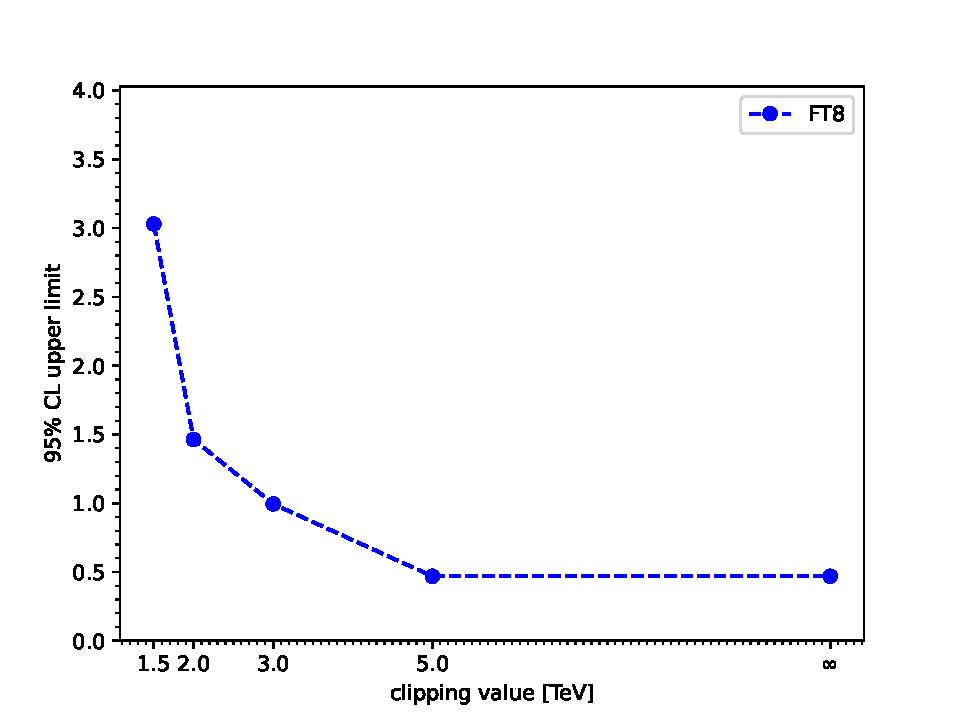
\includegraphics[width=0.32\textwidth]{figures/aQGC/ClippedFT8.pdf}}
%    	\subfigure[ FT9 ]{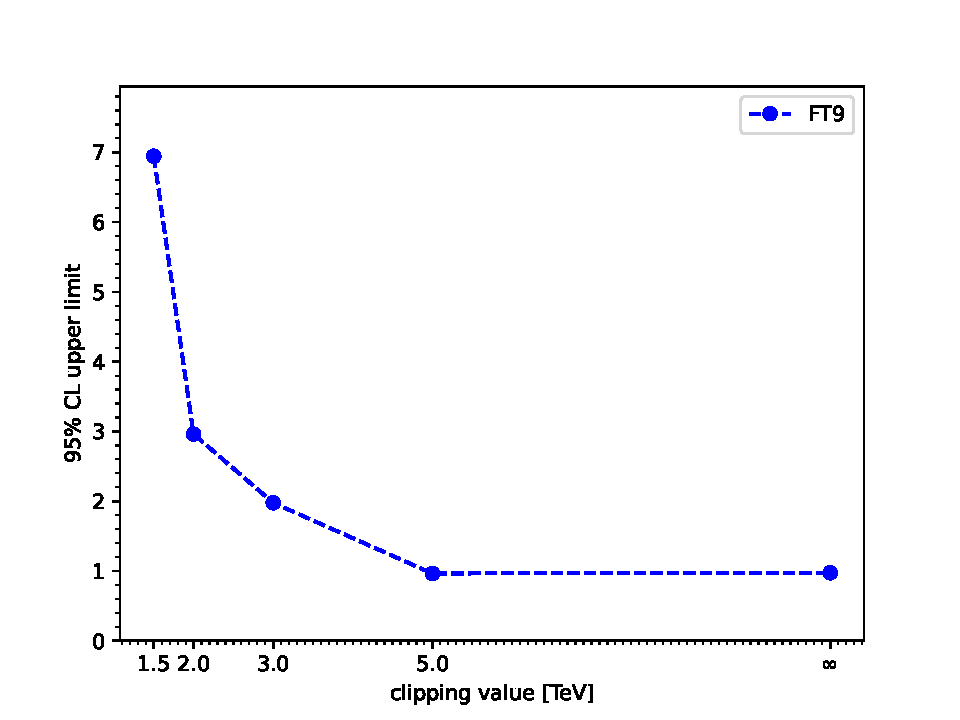
\includegraphics[width=0.32\textwidth]{figures/aQGC/ClippedFT9.pdf}}
%    	\subfigure[ FM0 ]{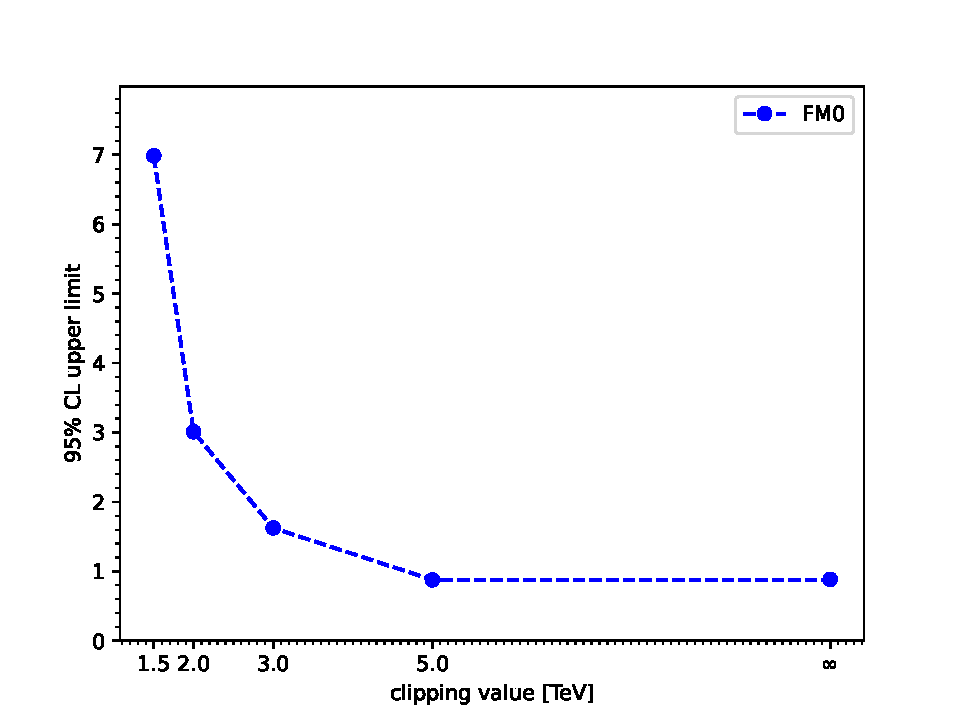
\includegraphics[width=0.32\textwidth]{figures/aQGC/ClippedFM0.pdf}}
%        \caption{Expected limits for 5 clipping points are shown for each coefficient FT8, FT9, and FM0.}
%\end{figure}
%
%\begin{figure}[ht]
%    \centering
%    	\subfigure[ FM1 ]{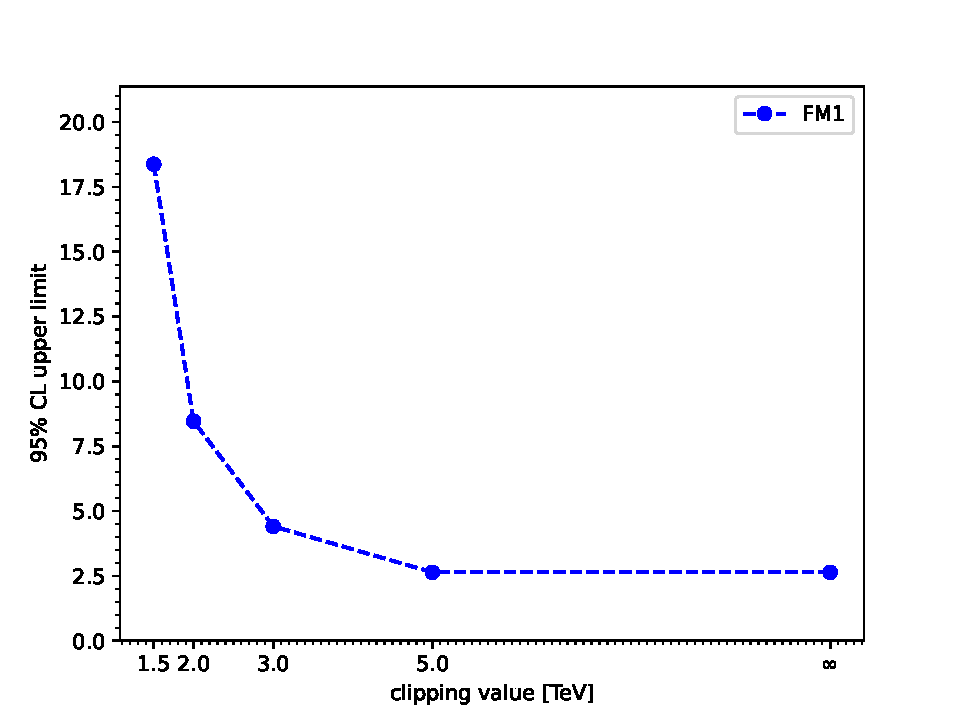
\includegraphics[width=0.32\textwidth]{figures/aQGC/ClippedFM1.pdf}}
%    	\subfigure[ FM2 ]{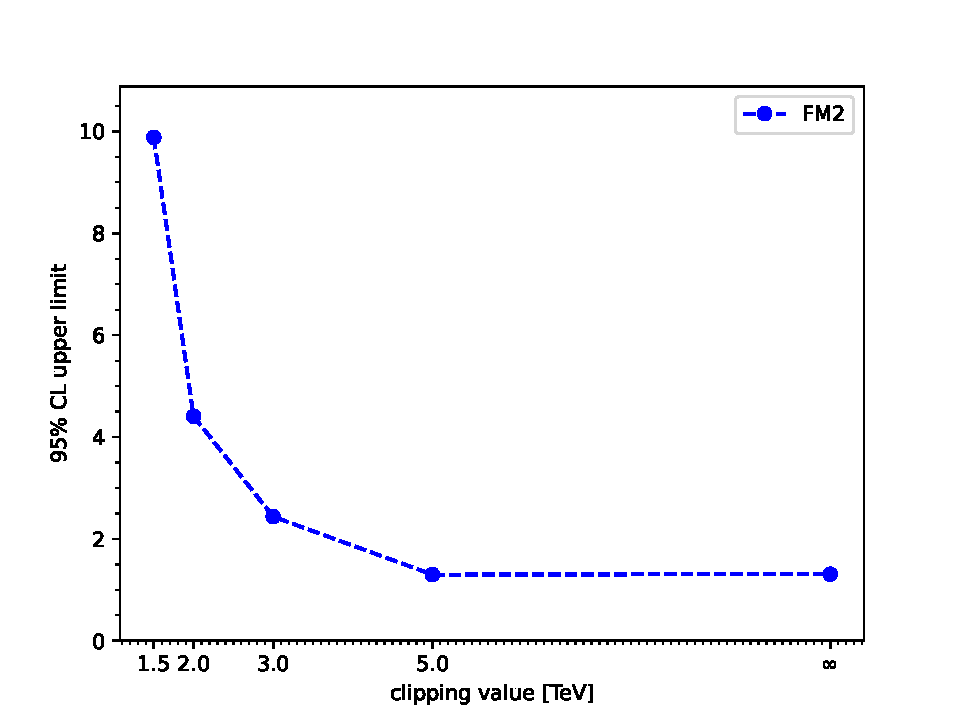
\includegraphics[width=0.32\textwidth]{figures/aQGC/ClippedFM2.pdf}}
%    	\subfigure[ FM3 ]{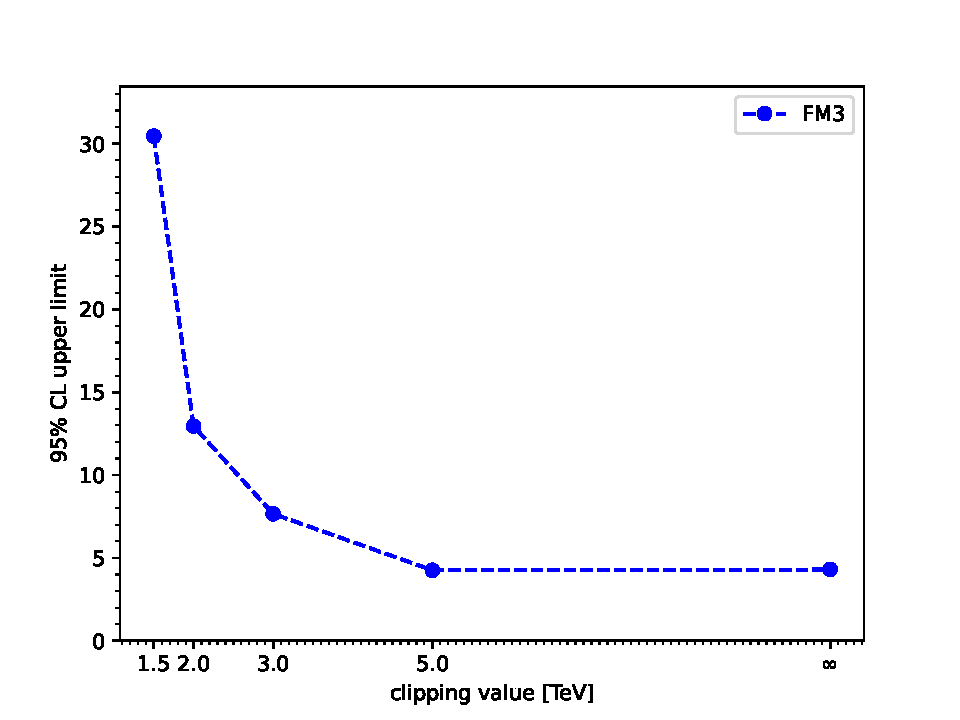
\includegraphics[width=0.32\textwidth]{figures/aQGC/ClippedFM3.pdf}}
%        \caption{Expected limits for 5 clipping points are shown for each coefficient FM1, FM2, and FM3.}
%\end{figure}
%
%\begin{figure}[ht]
%    \centering
%    	\subfigure[ FM4 ]{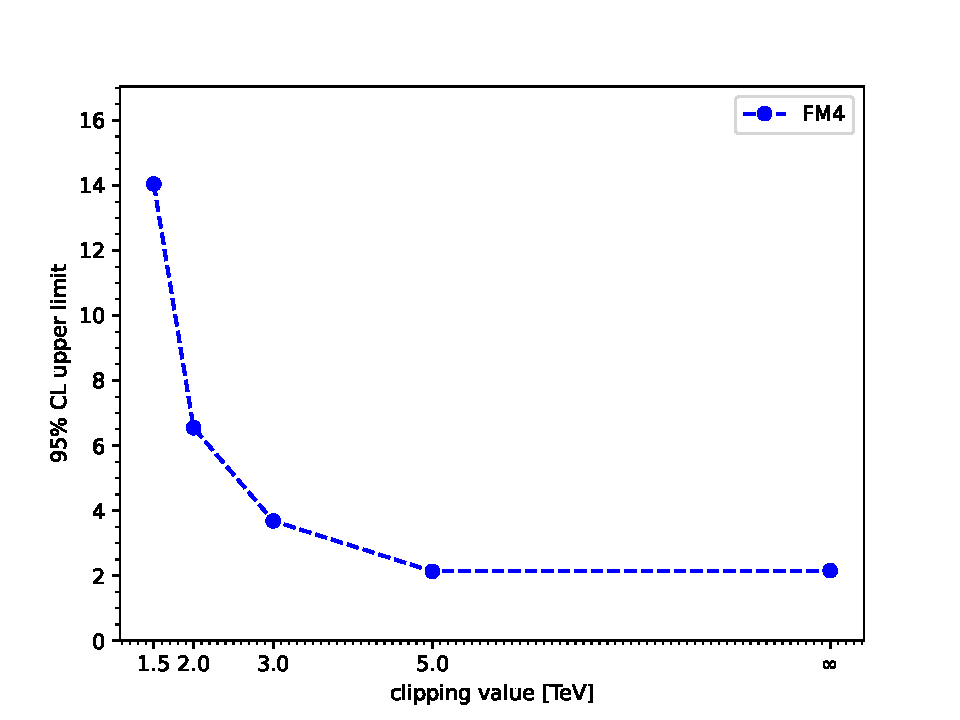
\includegraphics[width=0.32\textwidth]{figures/aQGC/ClippedFM4.pdf}}
%    	\subfigure[ FM5 ]{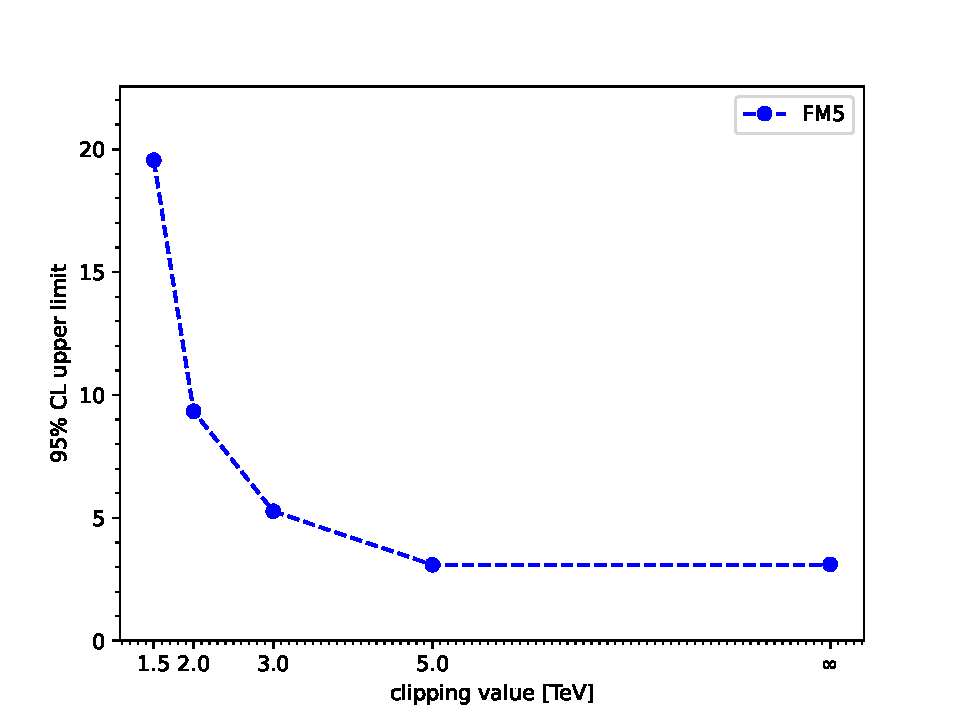
\includegraphics[width=0.32\textwidth]{figures/aQGC/ClippedFM5.pdf}}
%    	\subfigure[ FM7 ]{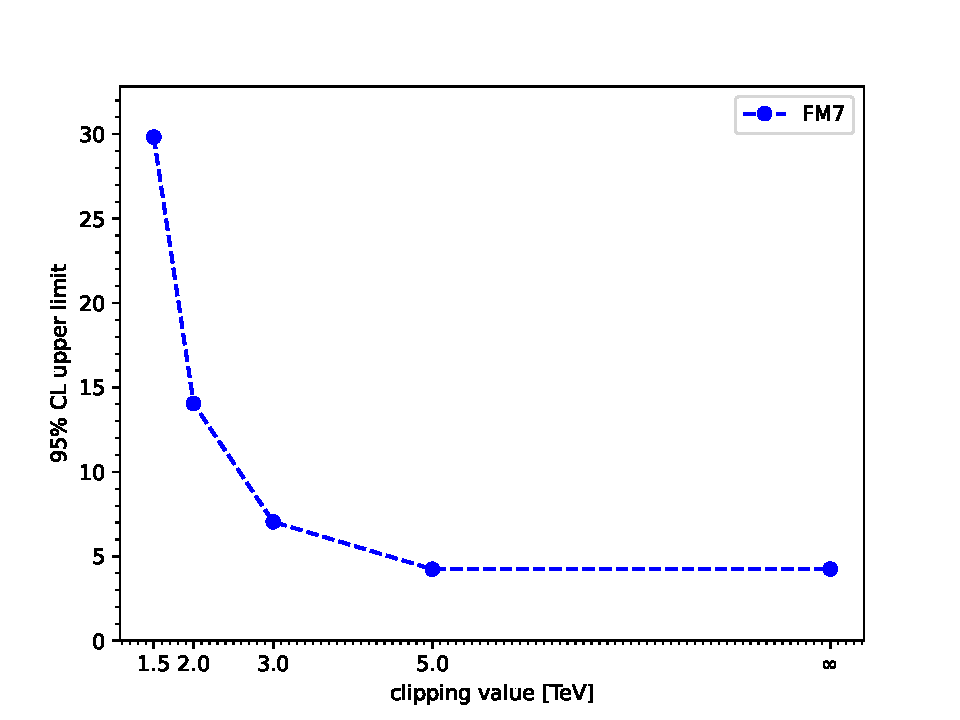
\includegraphics[width=0.32\textwidth]{figures/aQGC/ClippedFM7.pdf}}
%        \caption{Expected limits for 5 clipping points are shown for each coefficient FT4, FT5, and FM7.}
%\end{figure}
%
%\begin{figure}[ht]
%    \centering
%    	\subfigure[ FS02 ]{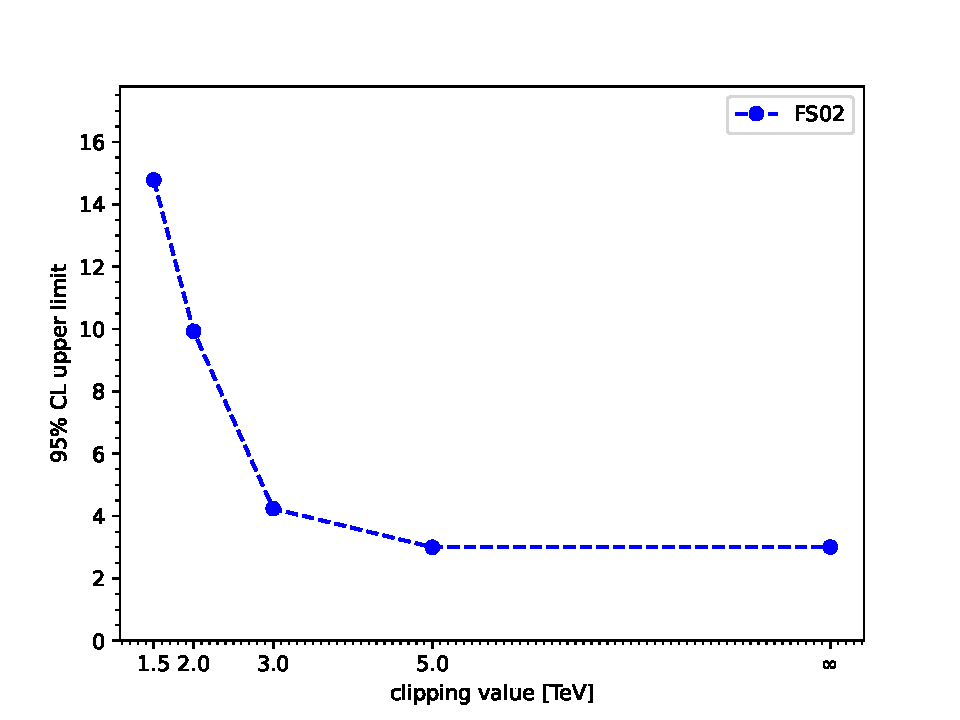
\includegraphics[width=0.32\textwidth]{figures/aQGC/ClippedFS02.pdf}}
%    	\subfigure[ FS1 ]{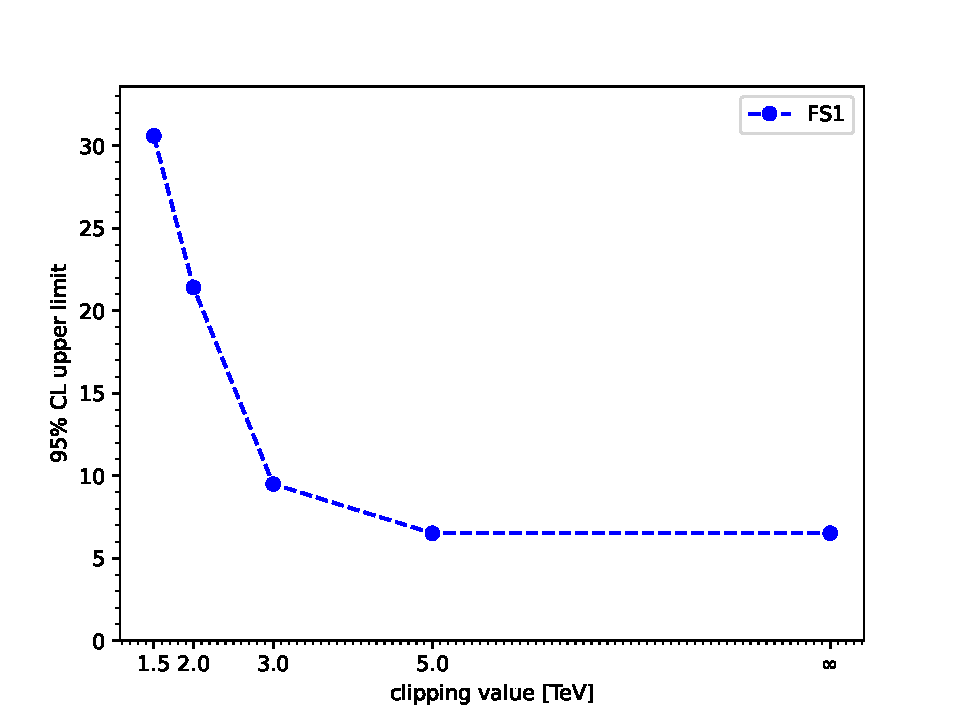
\includegraphics[width=0.32\textwidth]{figures/aQGC/ClippedFS1.pdf}}
%        \caption{Expected limits for 5 clipping points are shown for each coefficient FS02, FS1.}
%\end{figure}

\subsection{Initial study of the aQGC search strategy}
\label{subsec:binnedsig}

The aQGC terms can modify the amplitude of the VBS process at the higher effective center-of-mass energy, 
$m_{VV}$, as shown in Figure~\ref{fig:2lepaQGCshapeMVV}, hence merged regions are more important to enhance the signals.
Some studies below are based on Merged HP SR only.
It is found that the reconstructed $m_{VV}$ (or \mt\ in \zlep\ channel) is the best variable to separate the aQGC signals from the background,
while the RNN score distributions for the aQGC samples are similar to the one for the SM electroweak signal and still useful to suppress the non-VBS background as shown in Fig.~\ref{fig:2lepaQGCshapeRNN}.
Two-dimensional binning of $m_{VV}$ and the RNN score is used as the final discriminant for the aQGC search.
In this section, the optimal binning strategy is studied in \tlep\ channel.

\begin{figure}[]
    \centering
   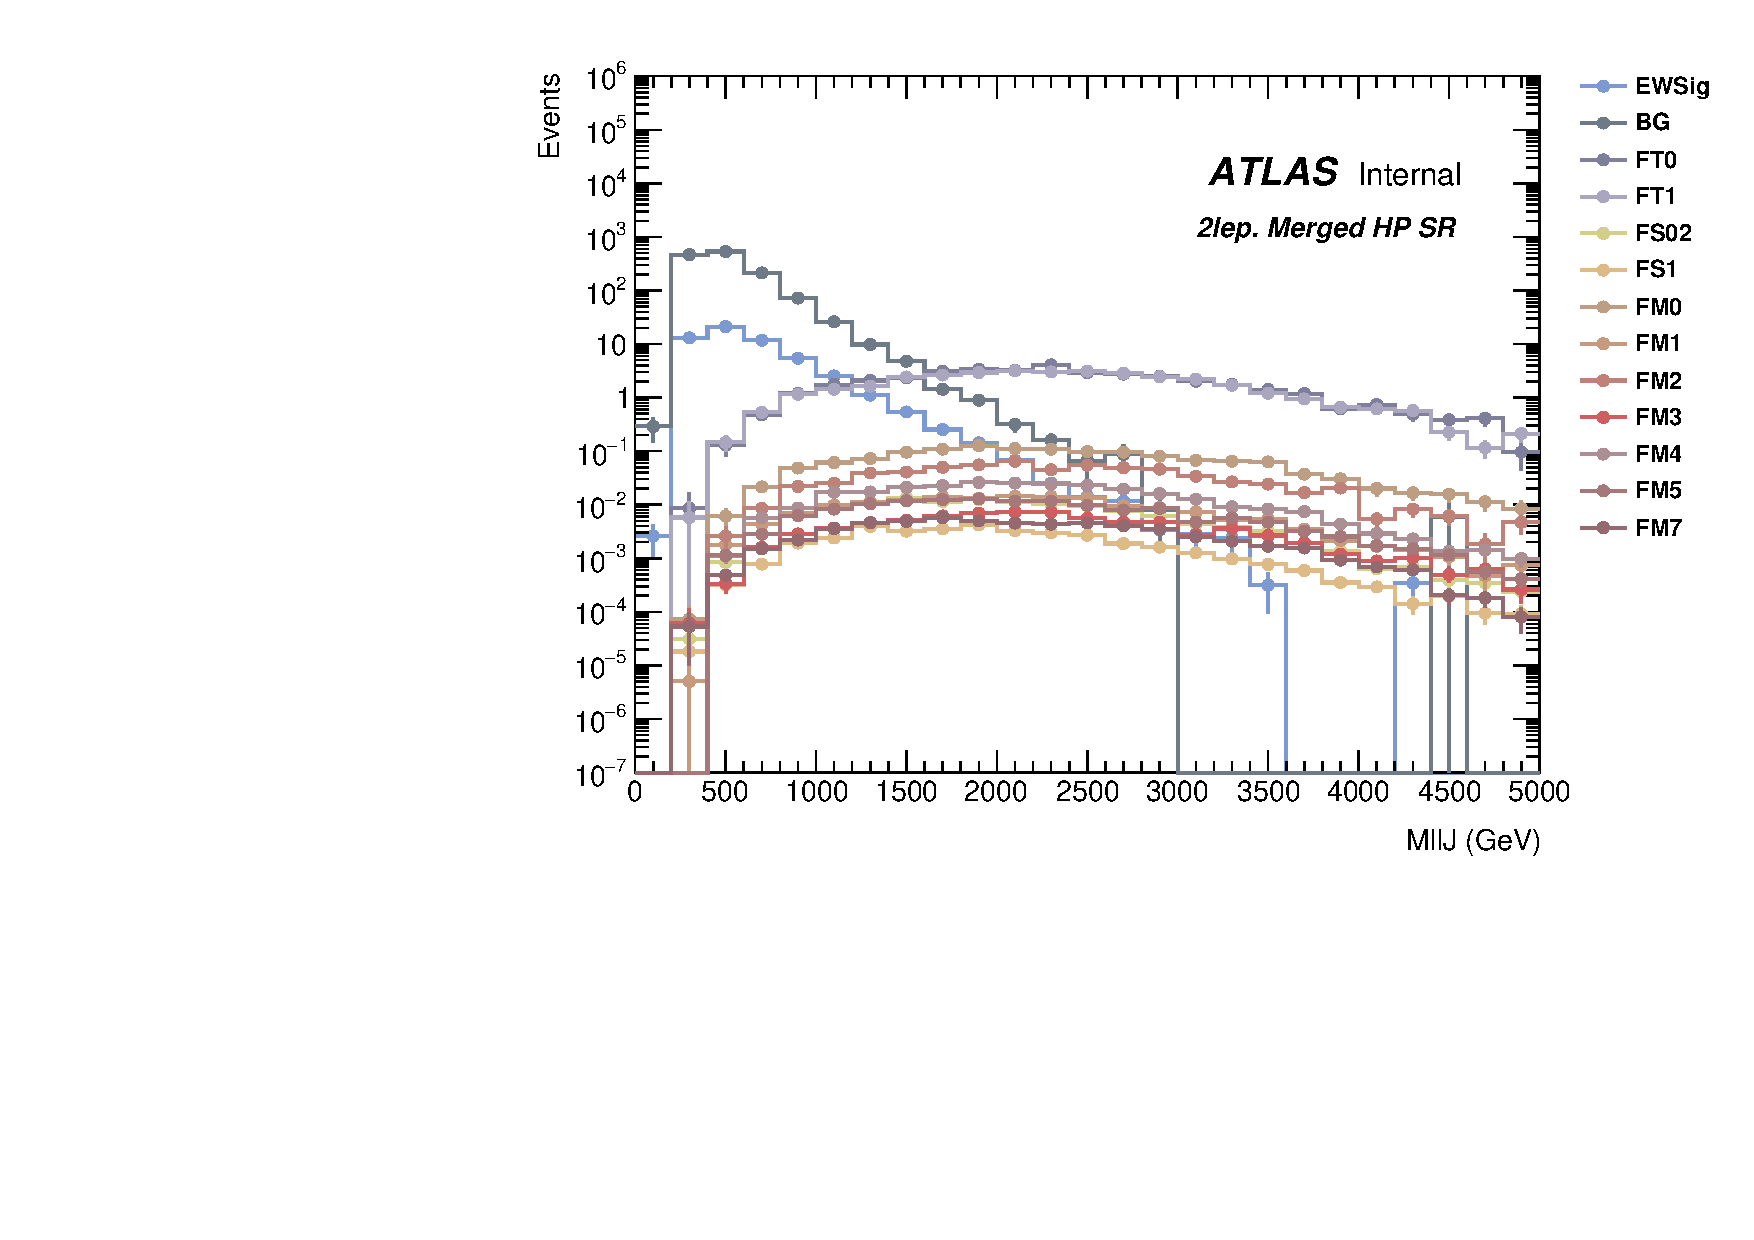
\includegraphics[width=0.45\textwidth]{figures/aQGC/MllJ_SR_HP_aQGC.pdf}
   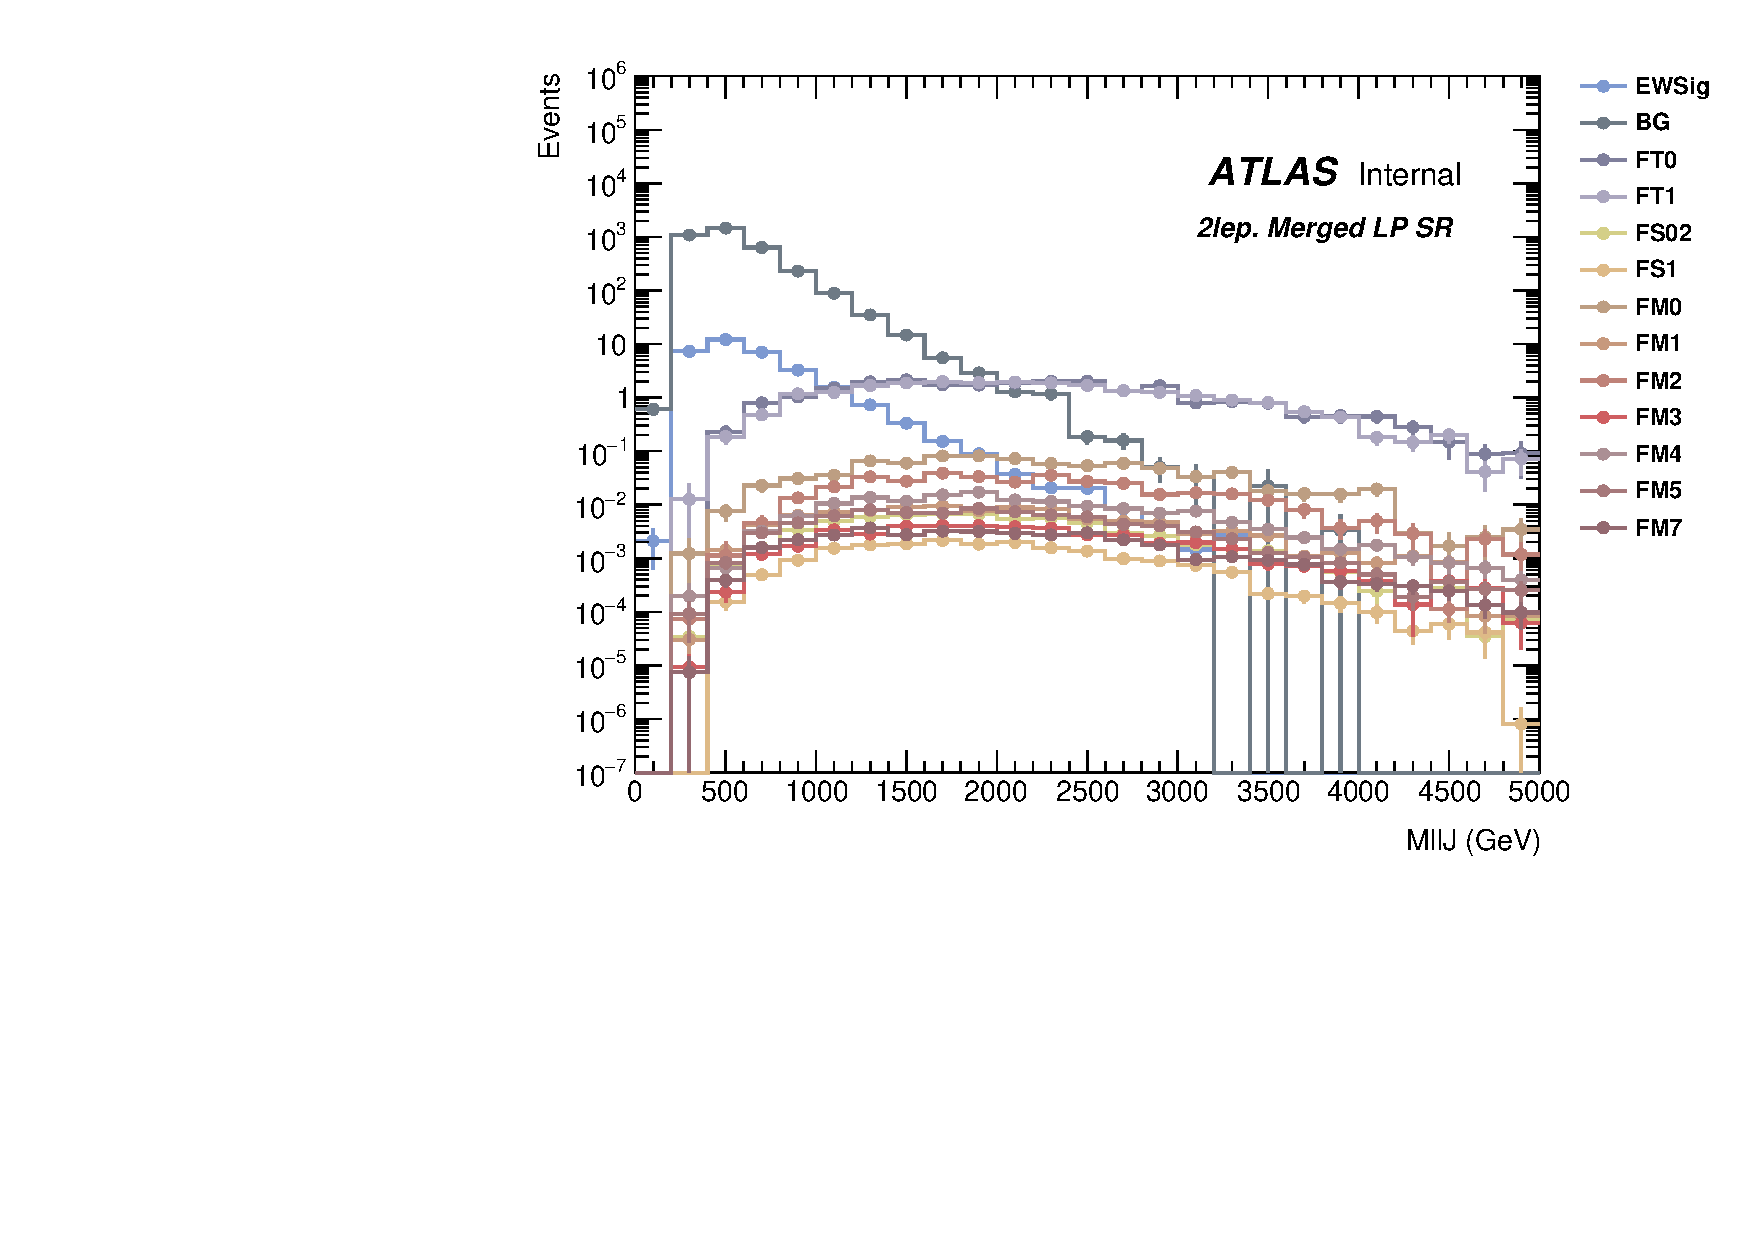
\includegraphics[width=0.45\textwidth]{figures/aQGC/MllJ_SR_LP_aQGC.pdf}
    \caption{$m_{VV}$ shape distribution of each wilson coefficient in Merged Signal regions. Only quadratic terms are shown.}
    \label{fig:2lepaQGCshapeMVV}
\end{figure}

\begin{figure}[]
    \centering
   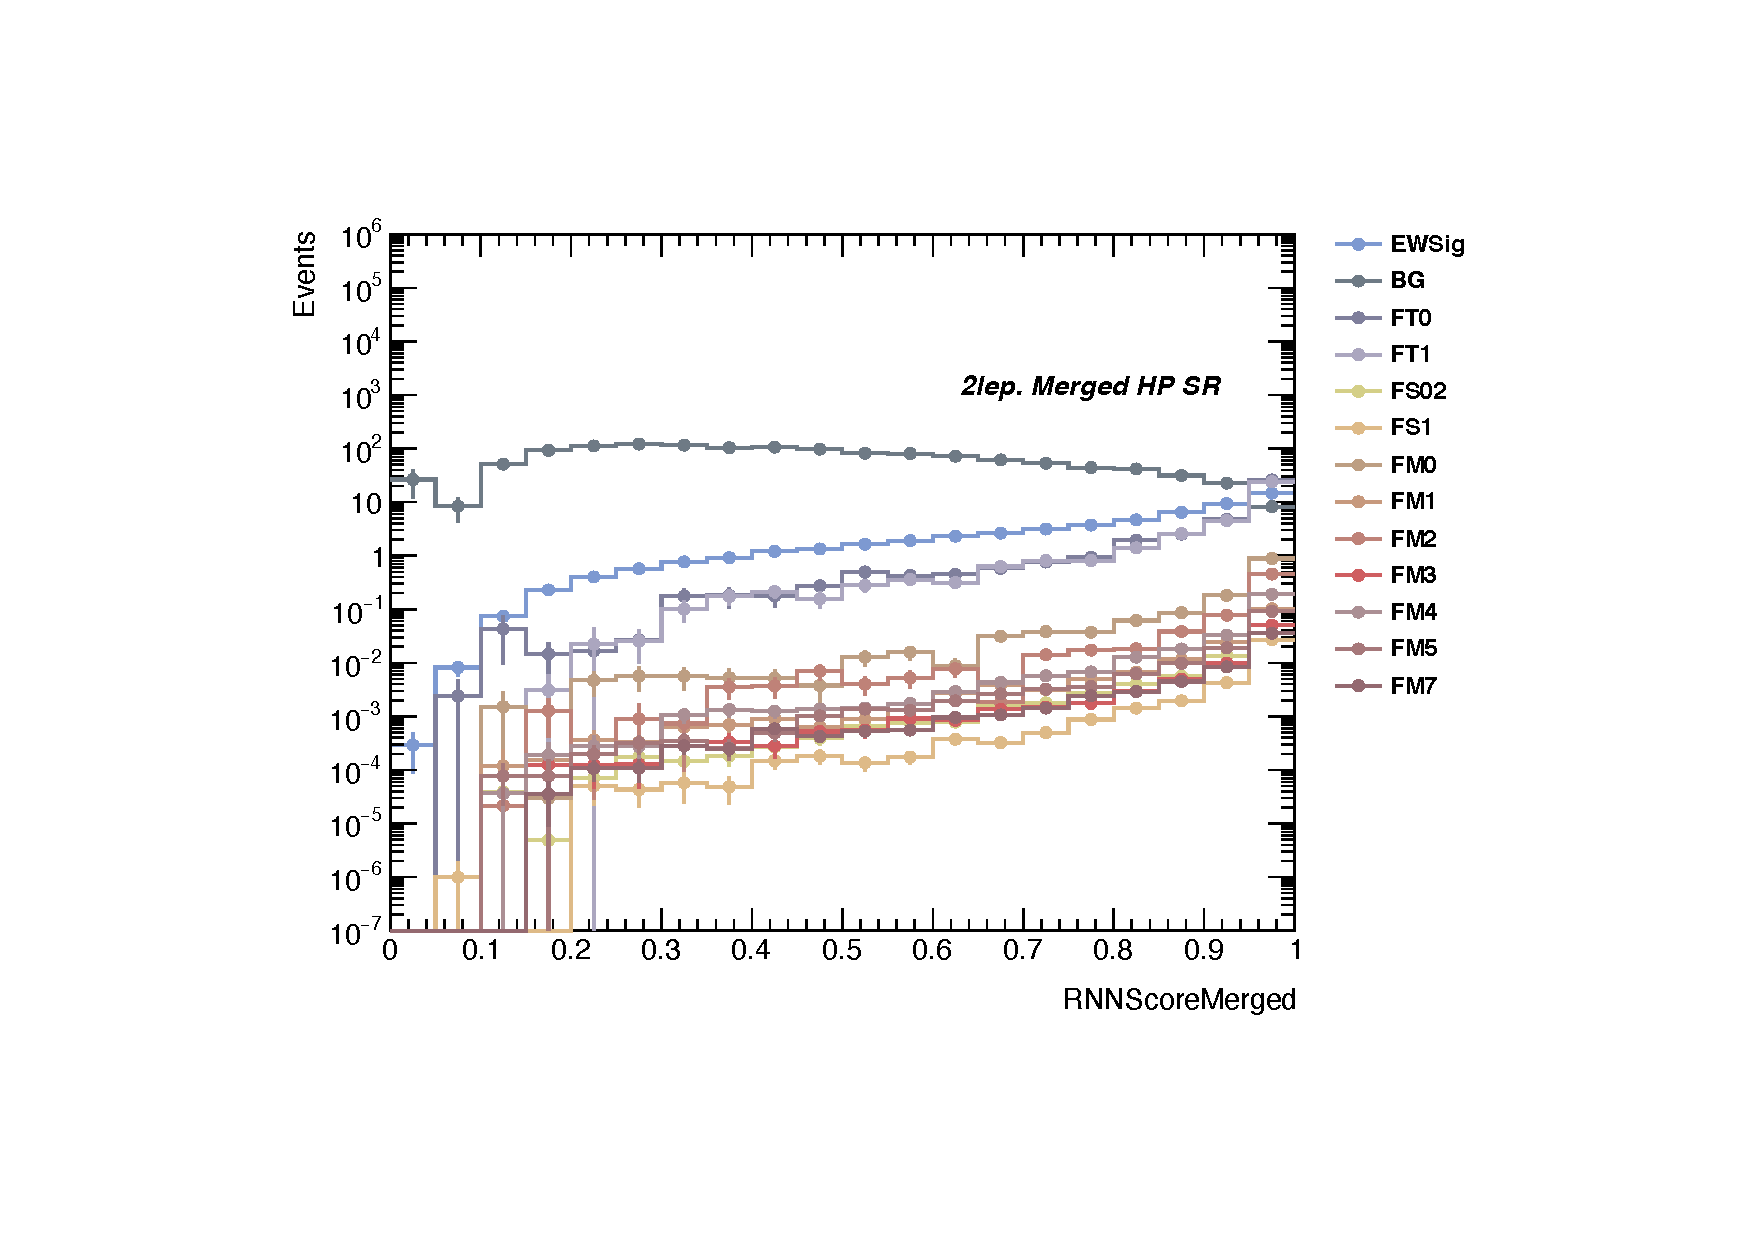
\includegraphics[width=0.45\textwidth]{figures/aQGC/RNNScoreMerged_SR_HP_aQGC.pdf}
   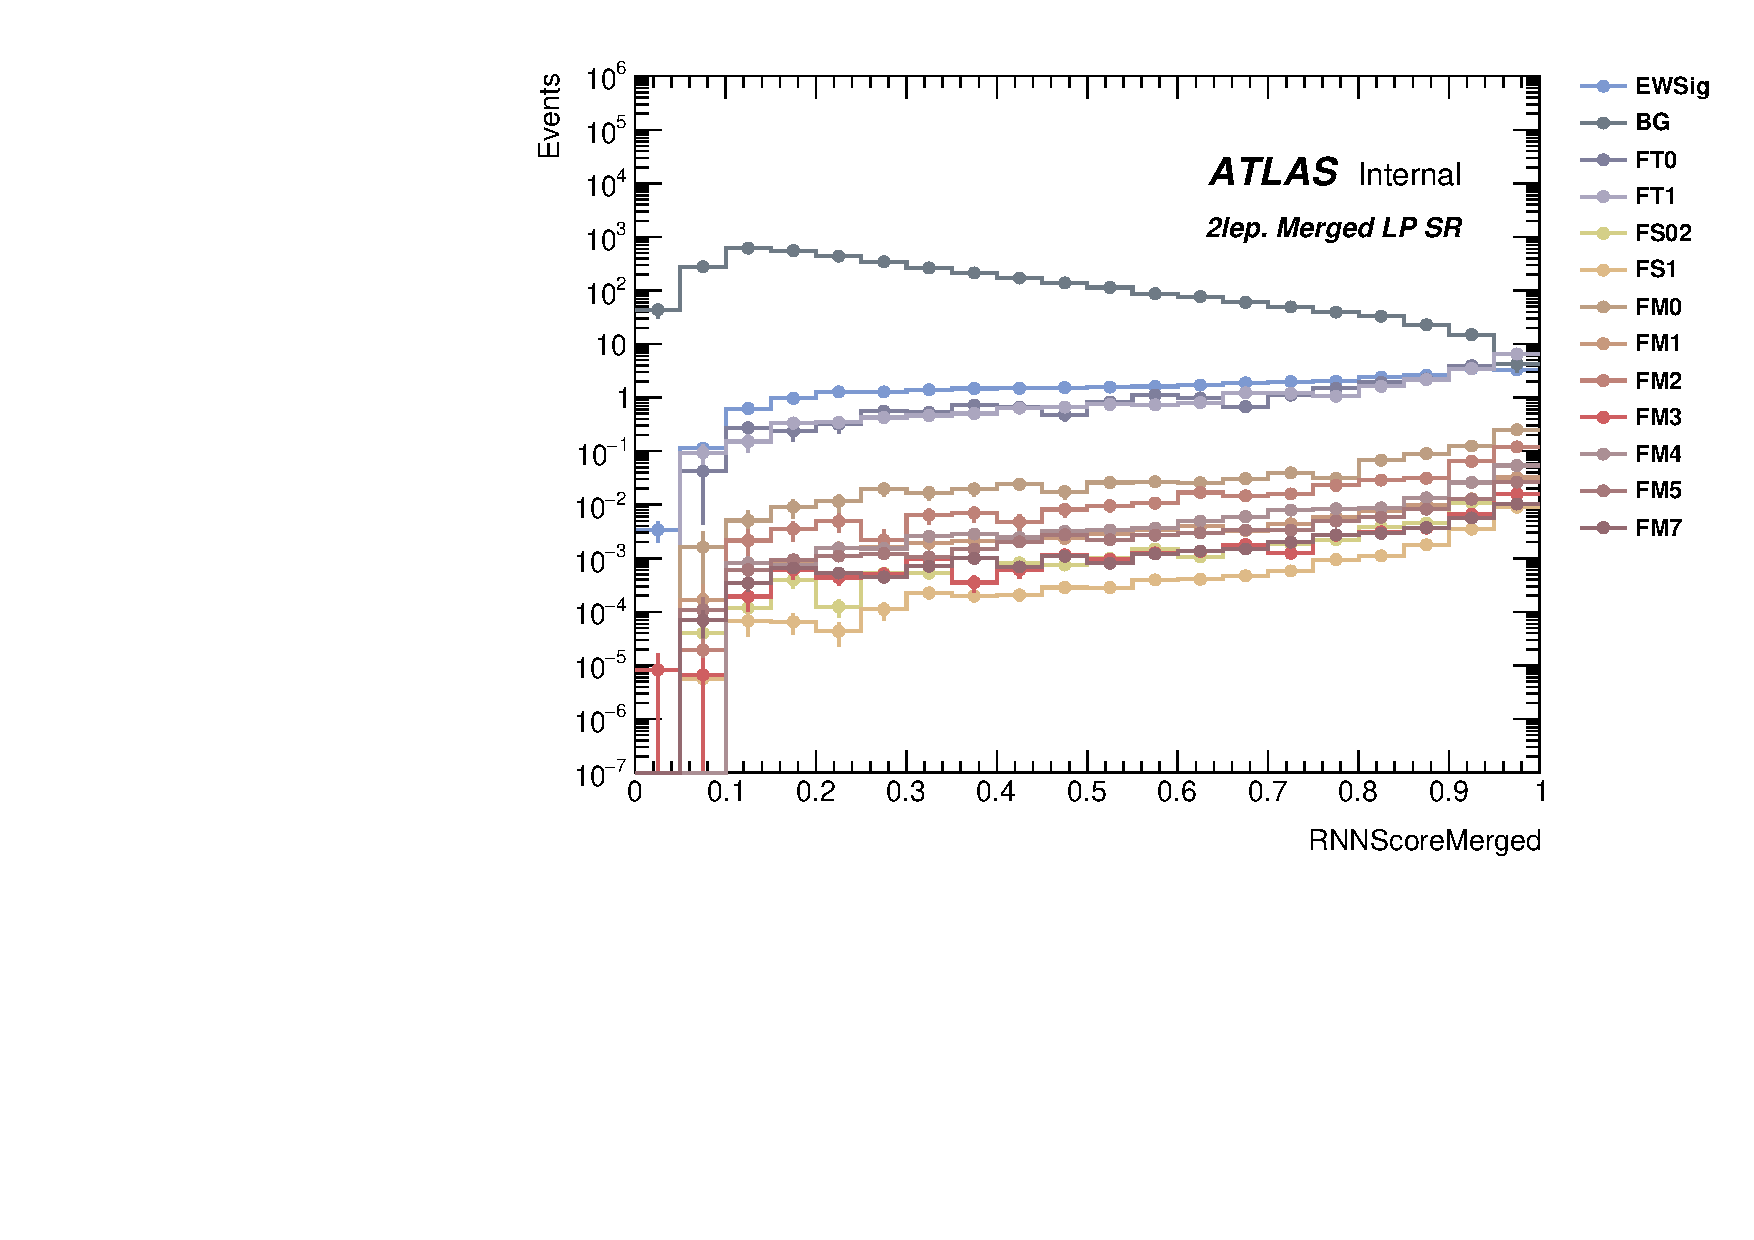
\includegraphics[width=0.45\textwidth]{figures/aQGC/RNNScoreMerged_SR_LP_aQGC.pdf}
    \caption{RNN score shape distribution of each wilson coefficient in Merged Signal regions. Only quadratic terms are shown.}
    \label{fig:2lepaQGCshapeRNN}
\end{figure}

The binned significance defined as:
%
\begin{eqnarray*}
  Z = \sqrt{\sum_{bins}\left[2(s + b)ln\left(\frac{(s + b)(b+\sigma^2_{b})}{b^2+(s+b)\sigma^2_{b}}\right) - \frac{b^2}{\sigma^2_{b}}ln\left(1+\frac{\sigma^2_{b}s}{b(b+\sigma^2_{b})}\right)\right]} \\
\end{eqnarray*}
%
is used in this study.
The $s$ is the number of the aQGC signal for the given wilson coefficient.
Signal samples are normalized to $\frac{f_{i}}{\Lambda^4}=1.0$ and no clipping energy requirement described in Section~\ref{subsec:clipping} is applied. Only the quadratic term is used in this study since the interference term is negligibly small with this parameter choice.
The $b$ includes the SM electroweak signals and the other backgrounds (like $Z$+jets, \ttbar, QCD diboson).
The fractional systematic uncertainty $\sigma_{b} = 0.2$ is assumed.

For simplicity, and the background estimation stability by keeping the number of bins as small as possible, two different approaches are tested.
One is to use the $m_{VV}$ distribution for the binned significance definition, after the certain cut on the RNN score to suppress the SM background.
The other is to use the RNN score distribution for the binned significance calculation, after the cut on the $m_{VV}$ to enhance the aQGC signals.
We also varied the threshold for $\mathrm{M}_{tagjj}$ at the same time.

Figure~\ref{fig:2lepaQGCBinnedSigMVV} shows the binned significance calculated by using $m_{VV}$ distribution after the cuts on RNN score and $\mathrm{M}_{tagjj}$, as functions of the varied thresholds of them.
It is found a cut on RNN score does not help to improve the sensitivity so much,
and a cut on $\mathrm{M}_{tagjj}$ deteriorates it.
On the other hand, Figure~\ref{fig:2lepaQGCBinnedSigRNN} shows the binned significance by using RNN score distribution
after the cuts on $m_{VV}$ and $\mathrm{M}_{tagjj}$, as functions of the thresholds for them.
The result depends on the threshold for $m_{VV}$, depending on the signal strength (under the $f_i/\Lambda^4 = 1.0$ constraint, $f_{S}$ signals have smaller signal yields than $f_{T}$ and $f_{M}$ and tighter cut on $m_{VV}$ is preferred, but it is just a result of the arbitral choice).
The significance value for each wilson coefficient term is summarized in tables~\ref{tab:2lep_HPSR_MVV} to \ref{tab:2lep_LPSR_RNN}.
Generally, about 5--10\% better sensitivity can be obtained by using RNN score distribution after the cut on $m_{VV}$ at the certain threshold.

\begin{figure}[ht]
    \centering
    	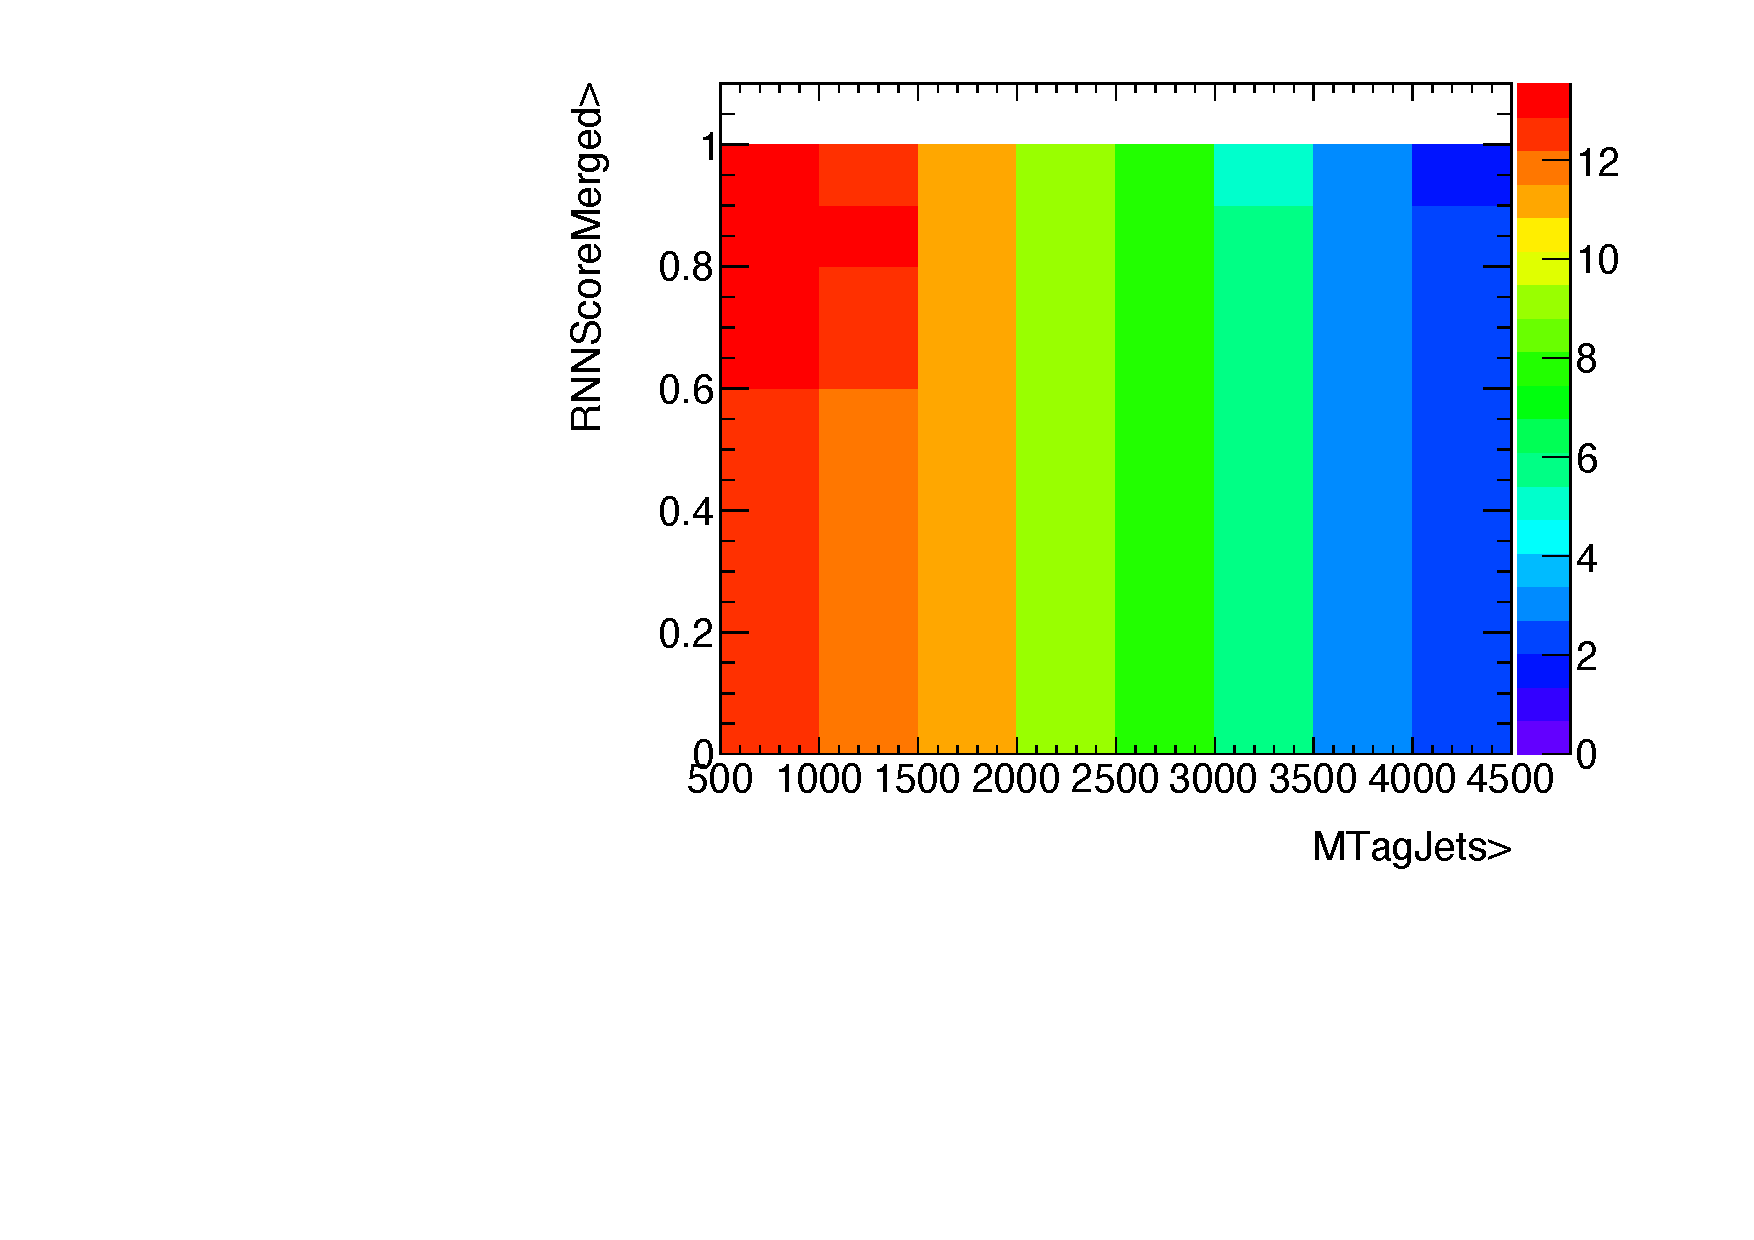
\includegraphics[width=0.30\textwidth]{figures/aQGC/HPSRFT0MVV.pdf}
    	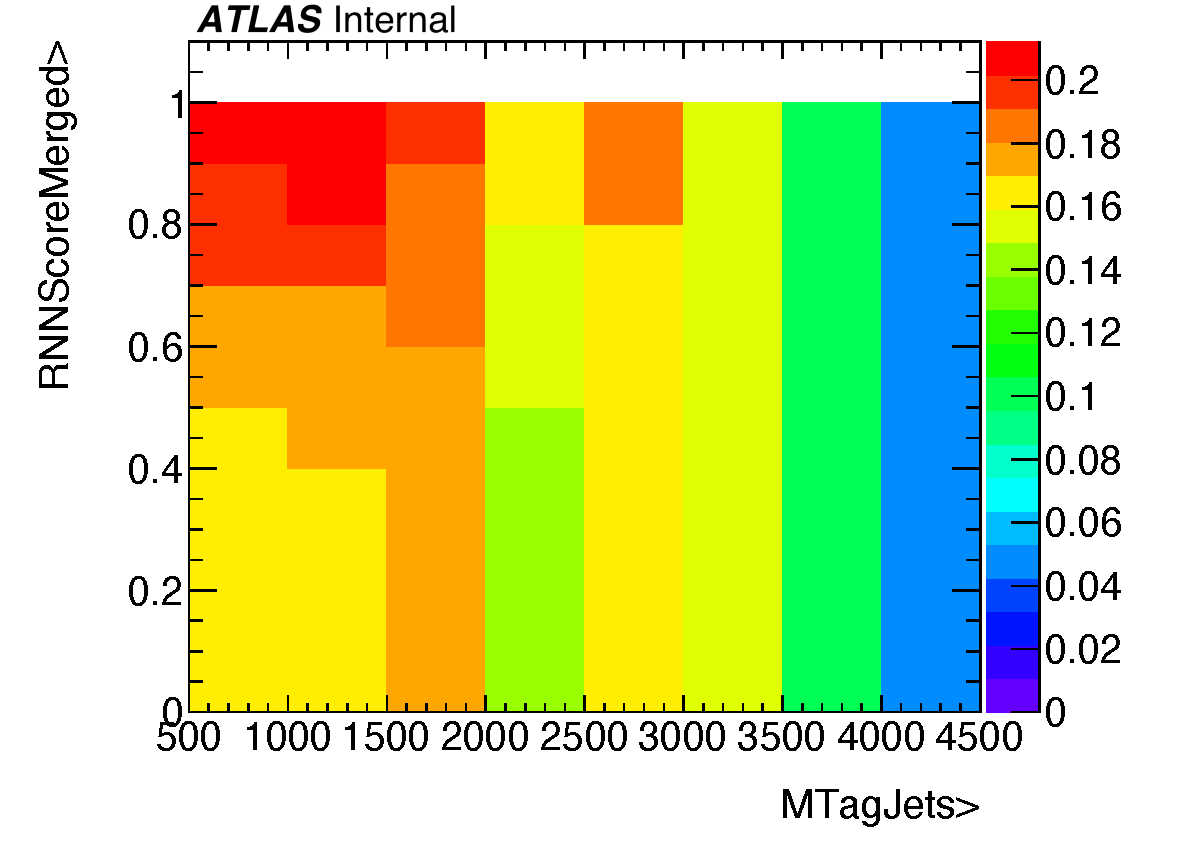
\includegraphics[width=0.30\textwidth]{figures/aQGC/HPSRFS02MVV.pdf}
        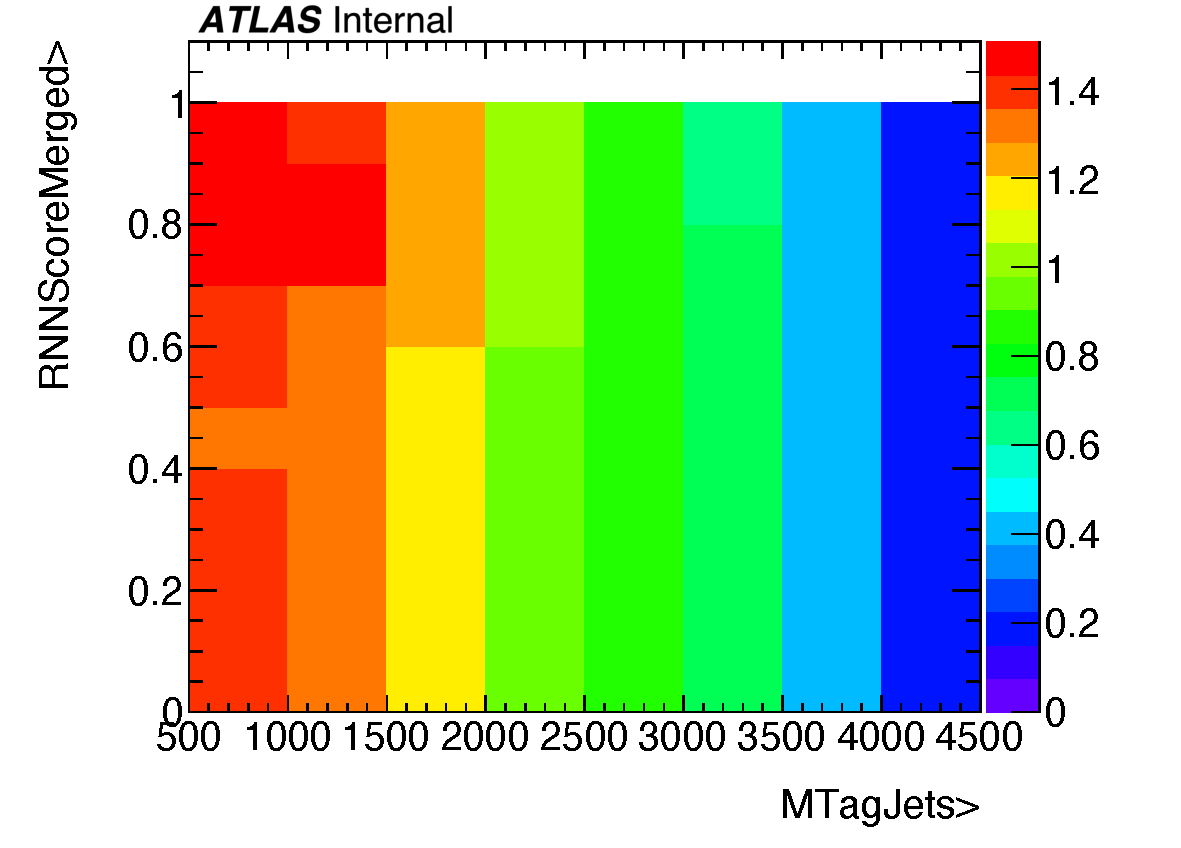
\includegraphics[width=0.30\textwidth]{figures/aQGC/HPSRFM0MVV.pdf}
        \caption{The 2D scan of the binned significance of operator FT0 (left), FS02 (middle), FM0 (right) with $m_{VV}$ score as discriminant in Merged HP signal region. Only quadratic terms are scanned.}
        \label{fig:2lepaQGCBinnedSigMVV}
\end{figure}

\begin{figure}[ht]
    \centering
    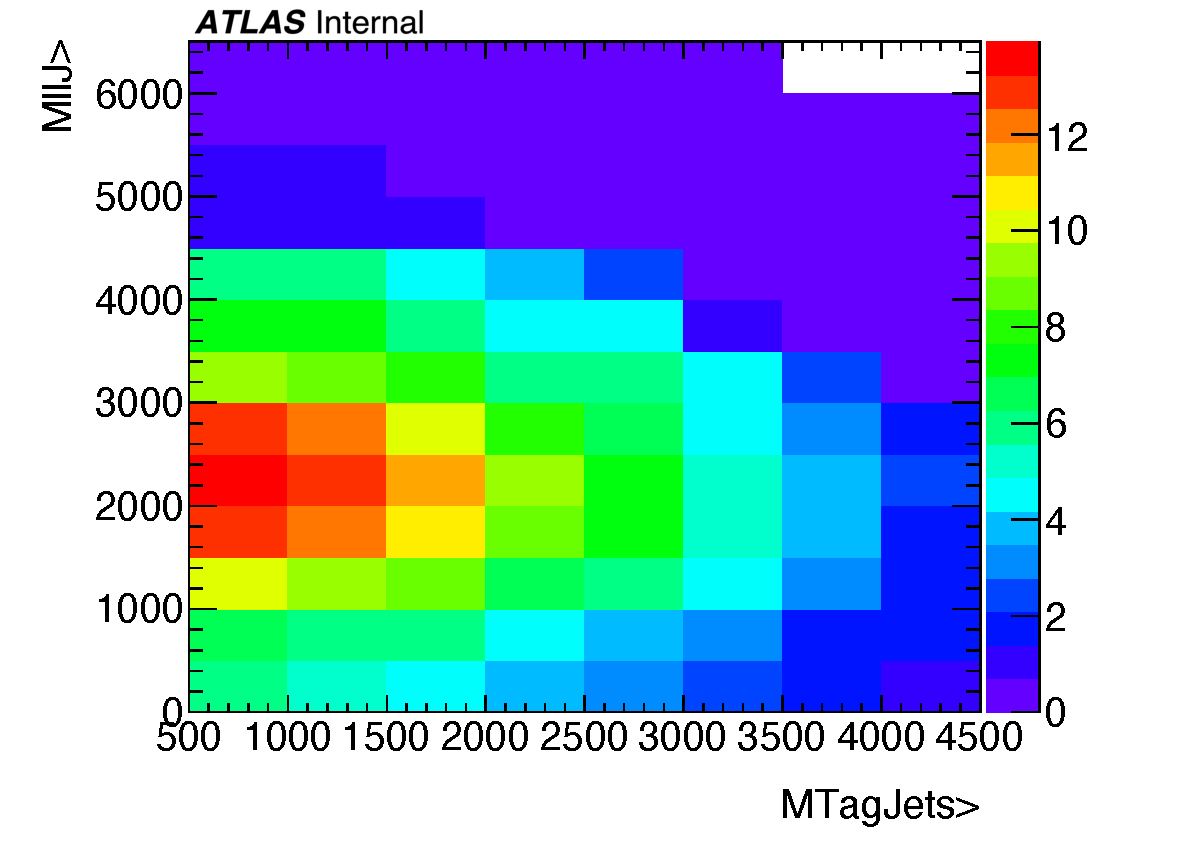
\includegraphics[width=0.30\textwidth]{figures/aQGC/HPSRFT0RNN.pdf}
    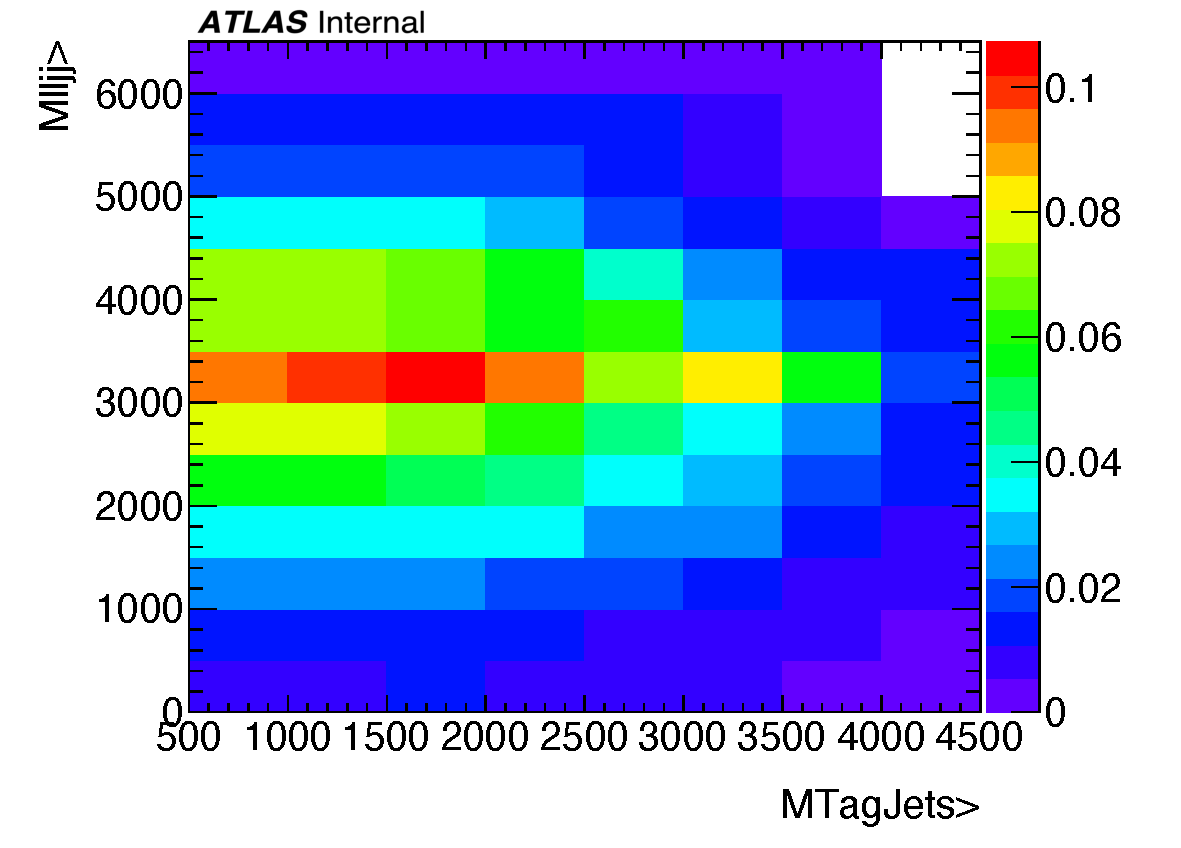
\includegraphics[width=0.30\textwidth]{figures/aQGC/HPSRFS02RNN.pdf}
  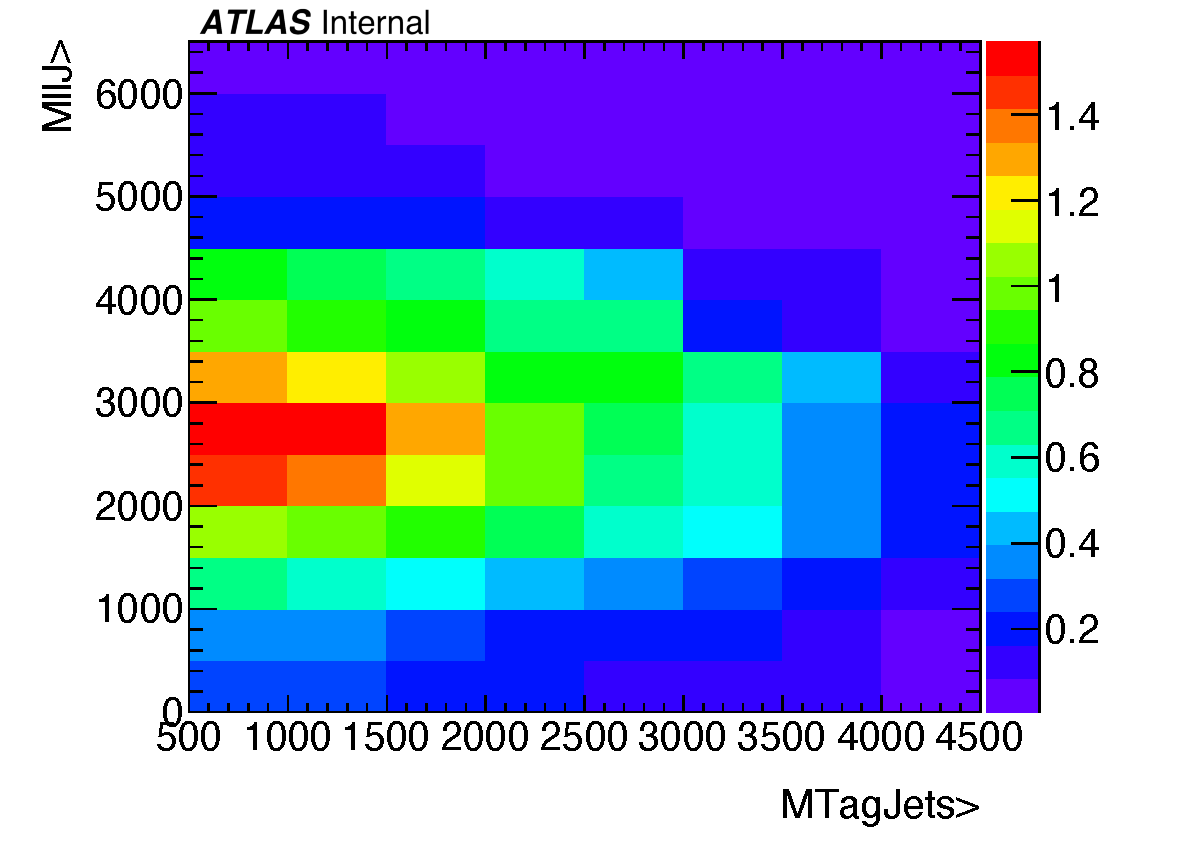
\includegraphics[width=0.30\textwidth]{figures/aQGC/HPSRFM0RNN.pdf}
        \caption{The 2D scan of the binned significance of operator FT0 (left), FS02 (middle), FM0 (right) with RNN score as discriminant in Merged HP signal region. Only quadratic terms are scanned.}
        \label{fig:2lepaQGCBinnedSigRNN}
\end{figure}

\begin{table}[ht!]
\small
\begin{center}
\resizebox{0.50\textwidth}{!}{

 \begin{tabular}{ r ||  r  r  r  r  |}
    & $\mathrm{M}_{tagjj}$ (GeV) & RNN score  & significance before cut& significance  \tabularnewline \hline
FT0 & 500                        & 0.6        & 12.55                  & 12.98         \tabularnewline \hline
FT1 & 500                        & 0.6        & 11.94                  & 12.50         \tabularnewline \hline
FS02& 1000                       & 0.8        & 0.17                   & 0.20          \tabularnewline \hline
FS1 & 500                        & 0.8        & 0.07                   & 0.07          \tabularnewline \hline
FM0 & 500                        & 0.7        & 1.36                   & 1.50          \tabularnewline \hline
FM1 & 500                        & 0.3        & 0.25                   & 0.27          \tabularnewline \hline
FM2 & 500                        & 0.7        & 0.82                   & 0.93          \tabularnewline \hline
FM3 & 500                        & 0.6        & 0.15                   & 0.16          \tabularnewline \hline
FM4 & 500                        & 0.7        & 0.38                   & 0.42          \tabularnewline \hline
FM5 & 500                        & 0.7        & 0.23                   & 0.25          \tabularnewline \hline
FM7 & 500                        & 0.6        & 0.12                   & 0.12          \tabularnewline \hline

\end{tabular}
}
\caption{Best cut point table for binned significance for $m_{VV}$ score distribution in \tlep channel in HPSR}
\label{tab:2lep_HPSR_MVV}
\end{center}
\end{table}

\begin{table}[ht!]
\small
\begin{center}
\resizebox{0.50\textwidth}{!}{

 \begin{tabular}{ r ||  r  r  r  r  |}
    & $\mathrm{M}_{tagjj}$ (GeV) & RNN score  & significance before cut & significance \tabularnewline \hline
FT0 & 500          & 0.1  & 6.65      & 6.77                          \tabularnewline \hline
FT1 & 500          & 0.2  & 6.69      & 6.85                          \tabularnewline \hline
FS02& 500          & 0.9  & 0.05      & 0.10                          \tabularnewline \hline
FS1 & 1000         & 0.8  & 0.02      & 0.04                          \tabularnewline \hline
FM0 & 500          & 0.8  & 0.54      & 0.12                          \tabularnewline \hline
FM1 & 500          & 0.1  & 0.08      & 0.42                          \tabularnewline \hline
FM2 & 500          & 0.9  & 0.28      & 0.08                          \tabularnewline \hline
FM3 & 1000         & 0.8  & 0.05      & 0.18                          \tabularnewline \hline
FM4 & 1000         & 0.8  & 0.12      & 0.10                          \tabularnewline \hline
FM5 & 1000         & 0.8  & 0.07      & 0.10                          \tabularnewline \hline
FM7 & 500          & 0.1  & 0.04      & 0.06                          \tabularnewline \hline

\end{tabular}
}
\caption{Best cut point table for binned significance for $m_{VV}$ score distribution in \tlep channel in LPSR}
\label{tab:2lep_LPSR_MVV}
\end{center}
\end{table}

\begin{table}[ht!]
\small
\begin{center}
\resizebox{0.50\textwidth}{!}{

 \begin{tabular}{ r ||  r  r  r  r  |}
    & $\mathrm{M}_{tagjj}$ (GeV) & MllJ (GeV) & significance before cut& significance \tabularnewline \hline
FT0 & 500          & 2000   & 5.62    & 13.92                           \tabularnewline \hline
FT1 & 500          & 2000   & 5.25    & 13.31                           \tabularnewline \hline
FS02& 1500         & 3000   & 0.01    & 0.11                            \tabularnewline \hline
FS1 & 2500         & 3000   & 0.01    & 0.07                            \tabularnewline \hline
FM0 & 500          & 2500   & 0.27    & 1.57                            \tabularnewline \hline
FM1 & 500          & 2500   & 0.03    & 0.28                            \tabularnewline \hline
FM2 & 500          & 2500   & 0.14    & 0.95                            \tabularnewline \hline
FM3 & 500          & 3000   & 0.01    & 0.12                            \tabularnewline \hline
FM4 & 500          & 2500   & 0.06    & 0.45                            \tabularnewline \hline
FM5 & 500          & 2500   & 0.03    & 0.25                            \tabularnewline \hline
FM7 & 500          & 2500   & 0.01    & 0.12                            \tabularnewline \hline

\end{tabular}
}
\caption{Best cut point table for binned significance for RNN score distribution in \tlep channel in HPSR}
\label{tab:2lep_HPSR_RNN}
\end{center}
\end{table}

\begin{table}[ht!]
\small
\begin{center}
\resizebox{0.50\textwidth}{!}{

 \begin{tabular}{ r ||  r  r  r  r  |}
    & $\mathrm{M}_{tagjj}$ (GeV) & MllJ (GeV) & significance before cut& significance \tabularnewline \hline
FT0 & 500          & 2000  & 2.64     & 7.72                            \tabularnewline \hline
FT1 & 500          & 2000  & 2.80     & 7.46                            \tabularnewline \hline
FS02& 1500         & 3000  & 0.01     & 0.06                            \tabularnewline \hline
FS1 & 500          & 3000  & 0.00     & 0.06                            \tabularnewline \hline
FM0 & 500          & 2500  & 0.12     & 0.92                            \tabularnewline \hline
FM1 & 500          & 3000  & 0.02     & 0.18                            \tabularnewline \hline
FM2 & 500          & 3000  & 0.06     & 0.54                            \tabularnewline \hline
FM3 & 500          & 3000  & 0.01     & 0.12                            \tabularnewline \hline
FM4 & 500          & 3000  & 0.03     & 0.26                            \tabularnewline \hline
FM5 & 500          & 3000  & 0.01     & 0.16                            \tabularnewline \hline
FM7 & 500          & 3000  & 0.01     & 0.09                            \tabularnewline \hline

\end{tabular}
}
\caption{Best cut point table for binned significance for RNN score distribution in \tlep channel LPSR}
\label{tab:2lep_LPSR_RNN}
\end{center}
\end{table}

Following the study of this section, a more reliable study based on the profile likelihood fit is performed
in Section~\ref{subsec:2binapproach}, using the RNN score as a discriminant after the cut on $m_{VV}$.

%\subsection{Expected limit}
%\label{subsec:aqgc_limit}

%The expected upper limit on each wilson coefficient by a combined fit of all 3 channels is shown in table~\ref{tab:aQGC_limit}, which is calculated by $\sqrt{\mu_{95\%}} = f_{i} / \Lambda^4$, where $\mu_{95\%}$ is the 95\% upper limit on the signal strength.
%The $m_{VV}$ distributions without any additional cuts are used in the fit.
%The systematic uncertainties are yet to be included.
%Figures~\ref{fig:0lepFT0} and ~\ref{fig:1lepFT0}, ~\ref{fig:2lepFT0} show the prefit plots of $m_{VV}$ distribution. FT0 signal is overlaid.

%\begin{table}[ht!]
%\small
%\begin{center}
%\resizebox{0.30\textwidth}{!}{
% \begin{tabular}{ | r || r |}
%    & Expected limit (TeV$^{-4})$ \tabularnewline \hline
%FT0 & 0.14                        \tabularnewline \hline
%FT1 & 0.14                        \tabularnewline \hline
%FS02& 2.90                        \tabularnewline \hline
%FS1 & 4.56e+6                     \tabularnewline \hline
%FM0 & 0.85                        \tabularnewline \hline
%FM1 & 2.55                        \tabularnewline \hline
%FM2 & 1.26                        \tabularnewline \hline
%FM3 & 4.69e+2                     \tabularnewline \hline
%FM4 & 2.07                        \tabularnewline \hline
%FM5 & 81.3                        \tabularnewline \hline
%FM7 & 5.37e+2                     \tabularnewline \hline
%\end{tabular}
%}
%\caption{Expected upper limits of each wilson coefficient. All 3 channels are combined.}
%\label{tab:aQGC_limit}
%\end{center}
%\end{table}
%
%\begin{figure}[ht]
%    \centering
%    	\subfigure[ 0lep merged CR ]{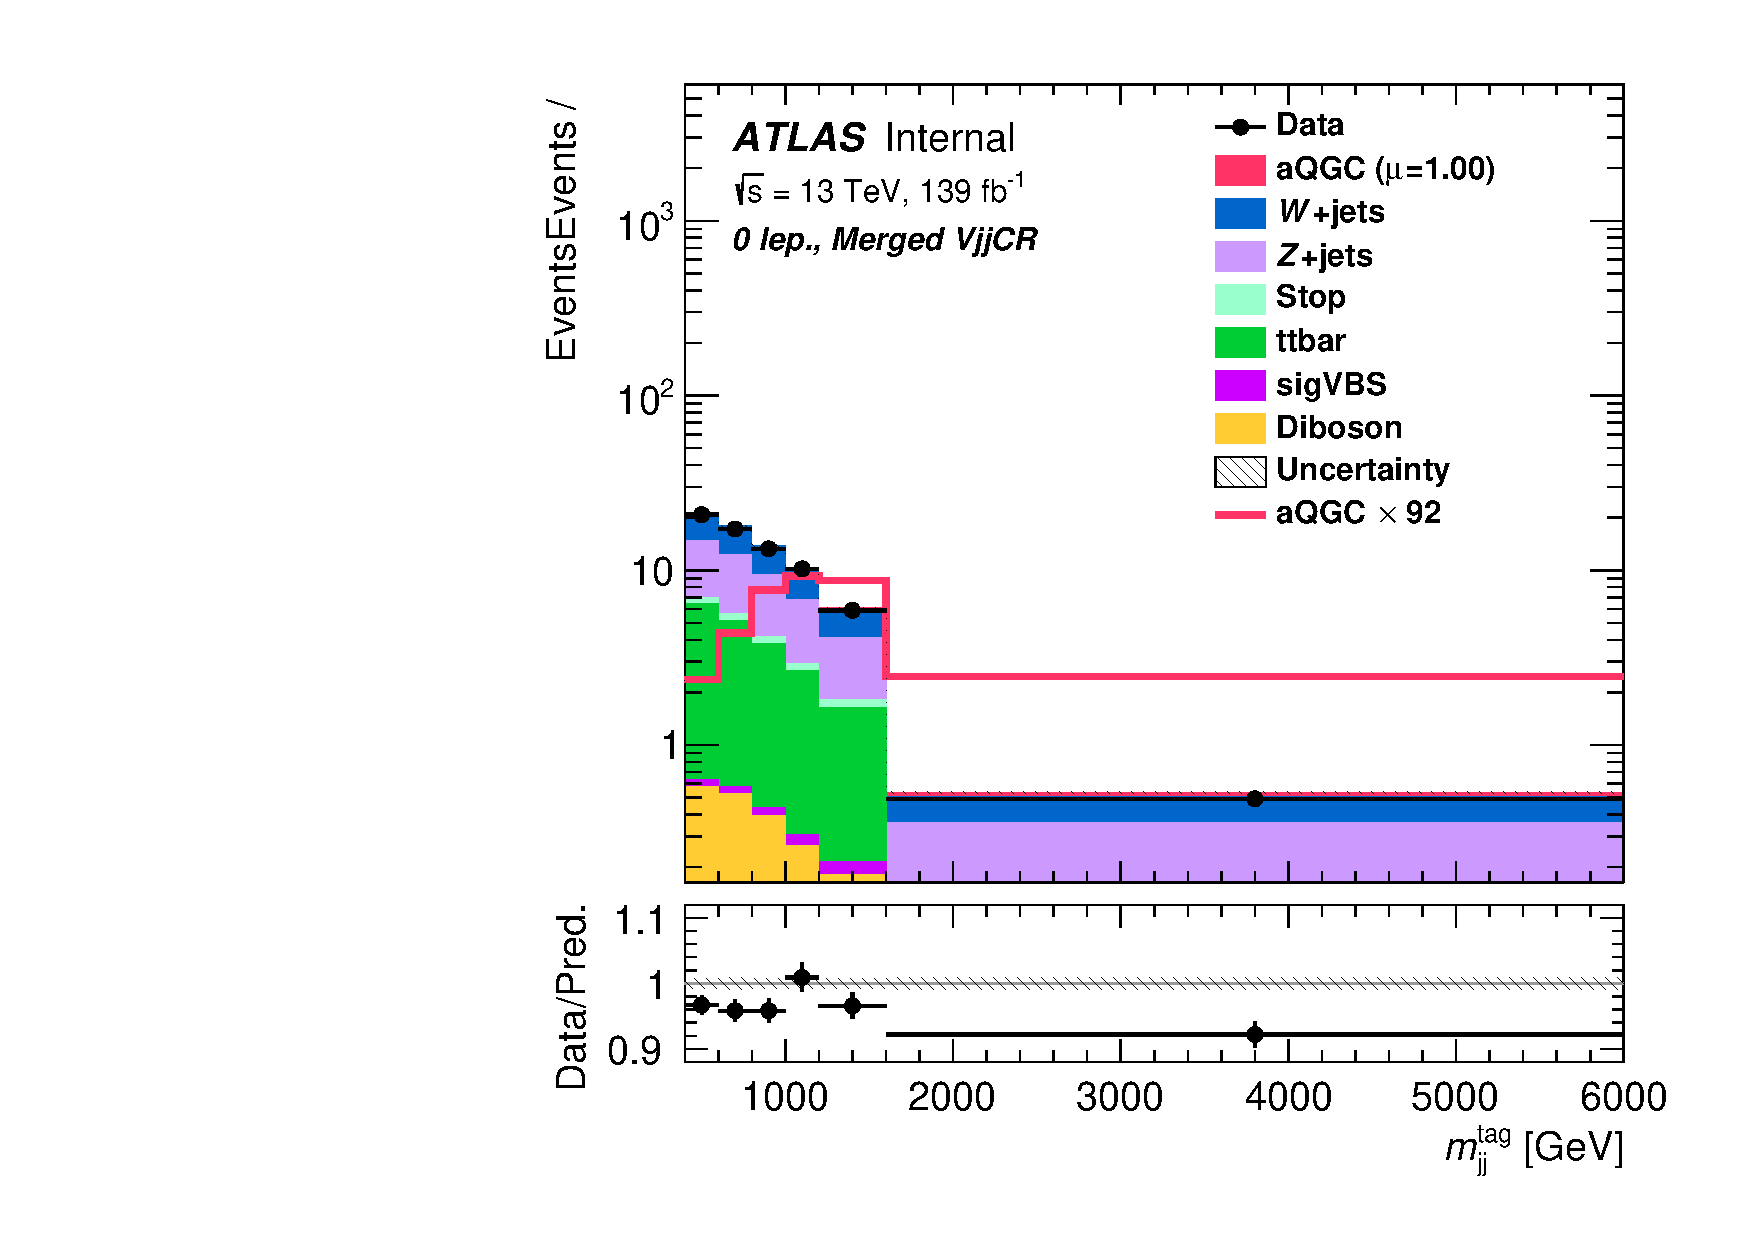
\includegraphics[width=0.32\textwidth]{figures/aQGC/Region_distMTagJets_DCRVjetMer_BMin0_J0_incJet1_L0_T0_incFat1_Y6051_incTag1_Fat1_Prefitlog.pdf}}
%    	\subfigure[ 0lep HP SR ]{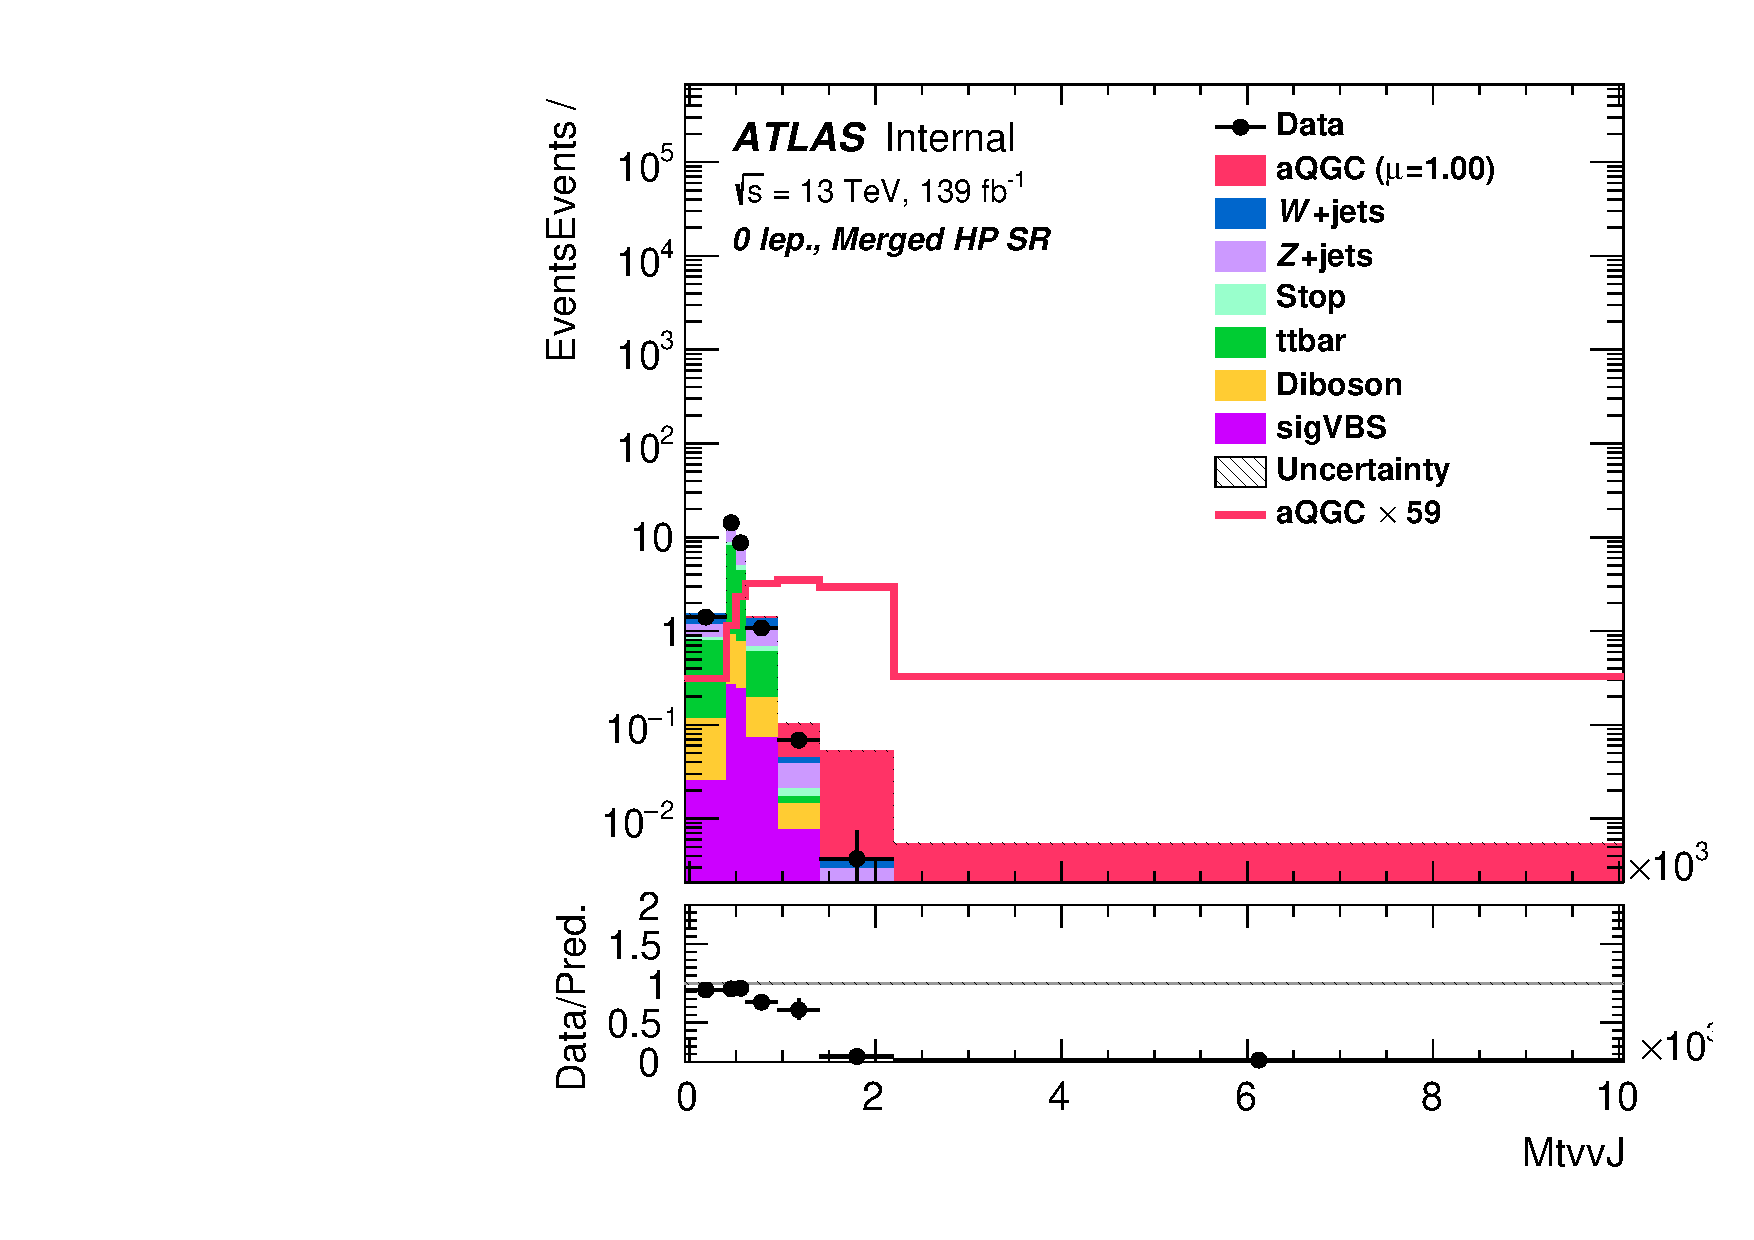
\includegraphics[width=0.32\textwidth]{figures/aQGC/Region_distMtvvJ_DSRVBSHP_BMin0_J0_incJet1_L0_T0_incFat1_Y6051_incTag1_Fat1_Prefitlog.pdf}}
%    	\subfigure[ 0lep LP SR ]{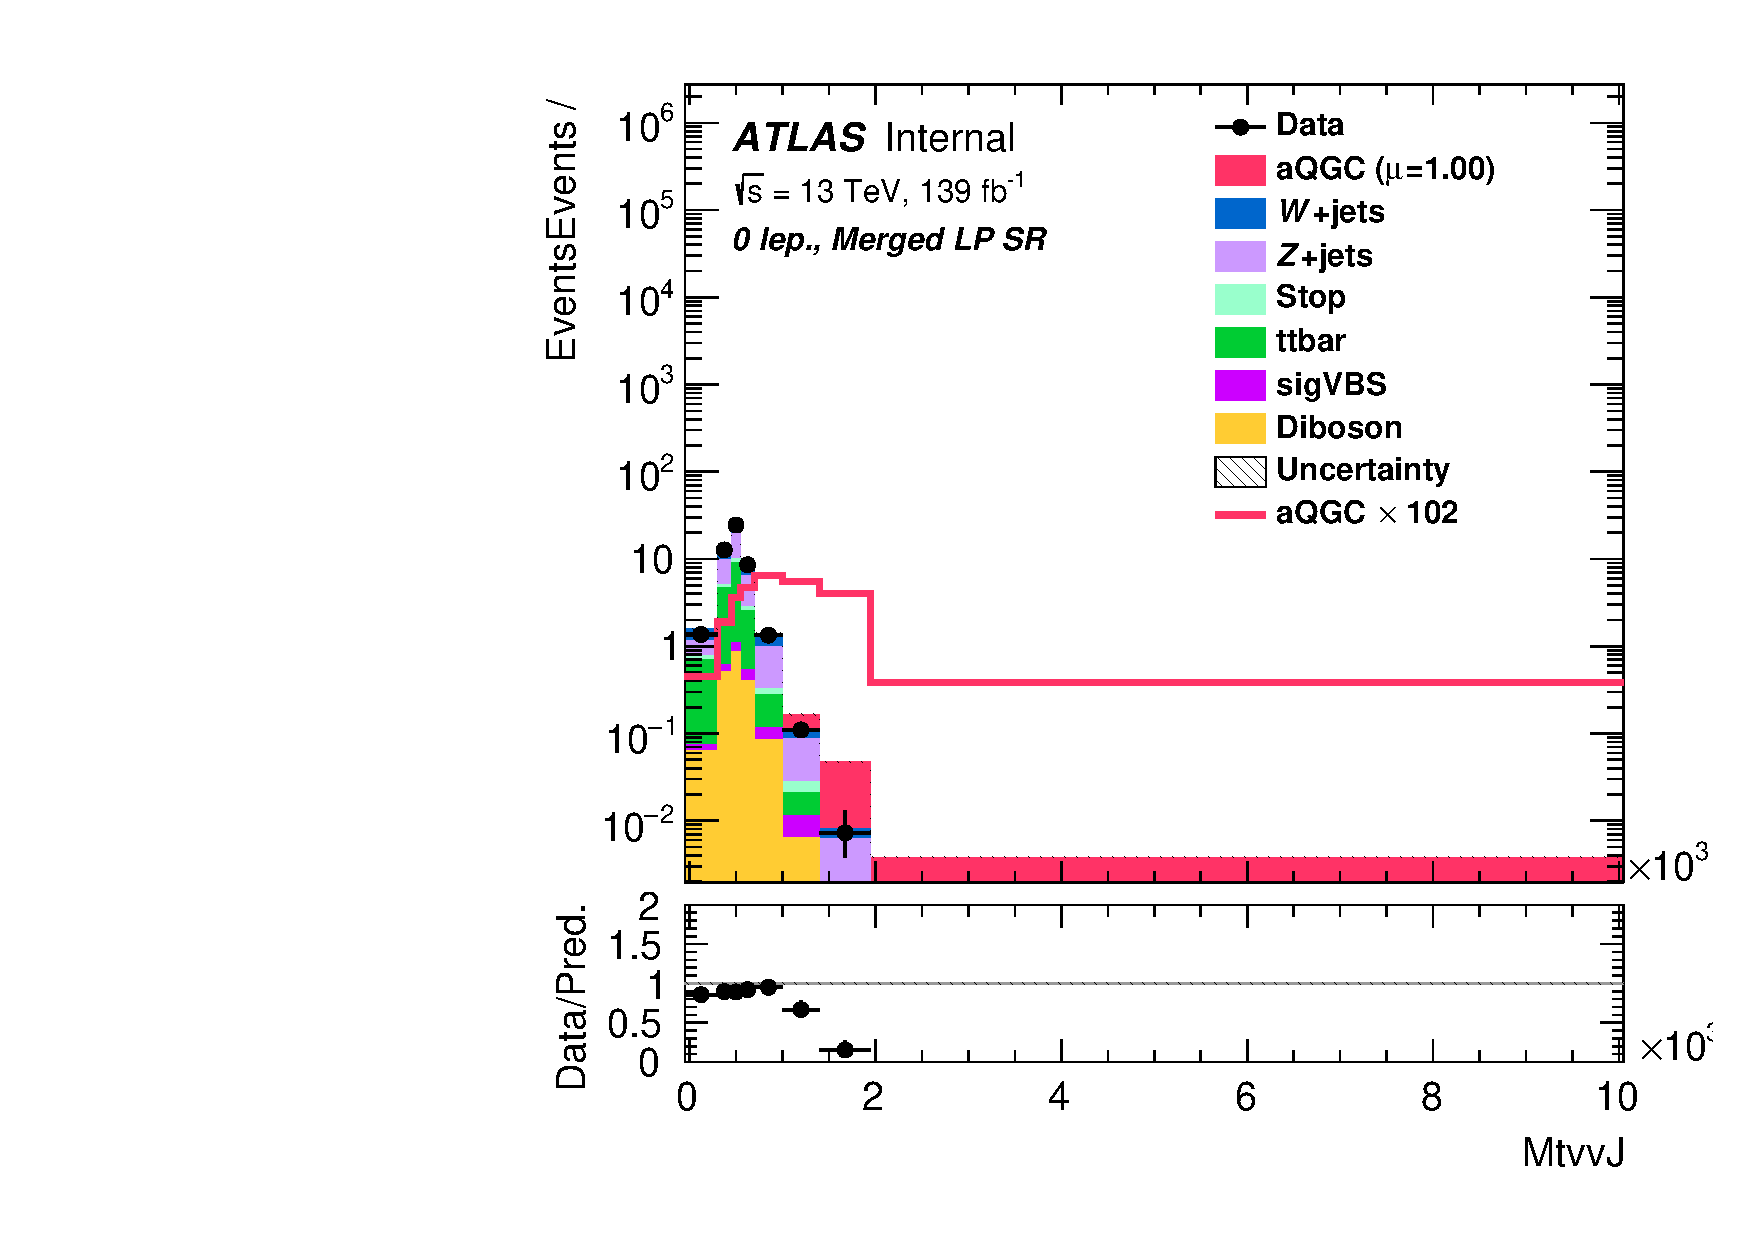
\includegraphics[width=0.32\textwidth]{figures/aQGC/Region_distMtvvJ_DSRVBSLP_BMin0_J0_incJet1_L0_T0_incFat1_Y6051_incTag1_Fat1_Prefitlog.pdf}}
%    	\subfigure[ 0lep resolved CR ]{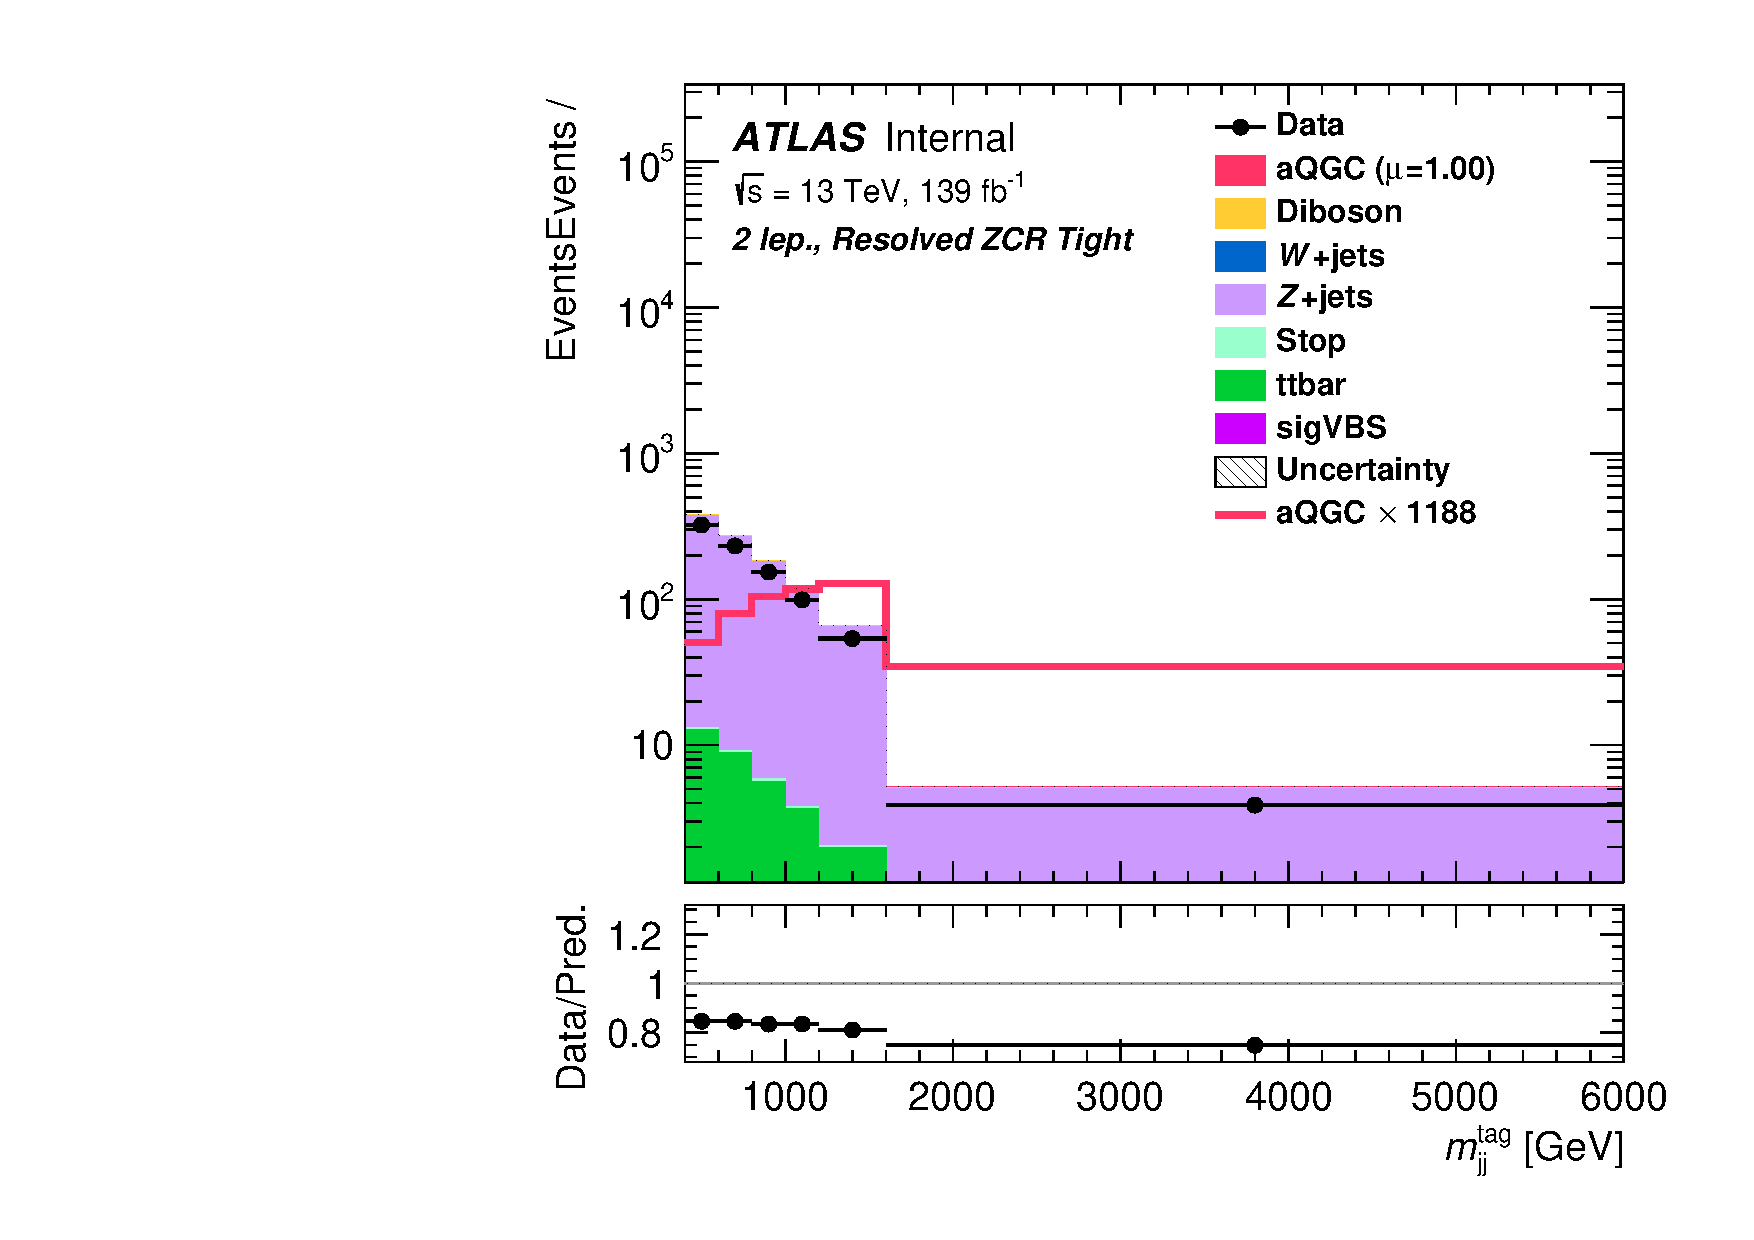
\includegraphics[width=0.32\textwidth]{figures/aQGC/Region_distMTagResJets_DCRVjetFid_BMin0_T0_Y6051_incTag1_J2_L2_incJet1_Prefitlog.pdf}}
%    	\subfigure[ 0lep resolved SR ]{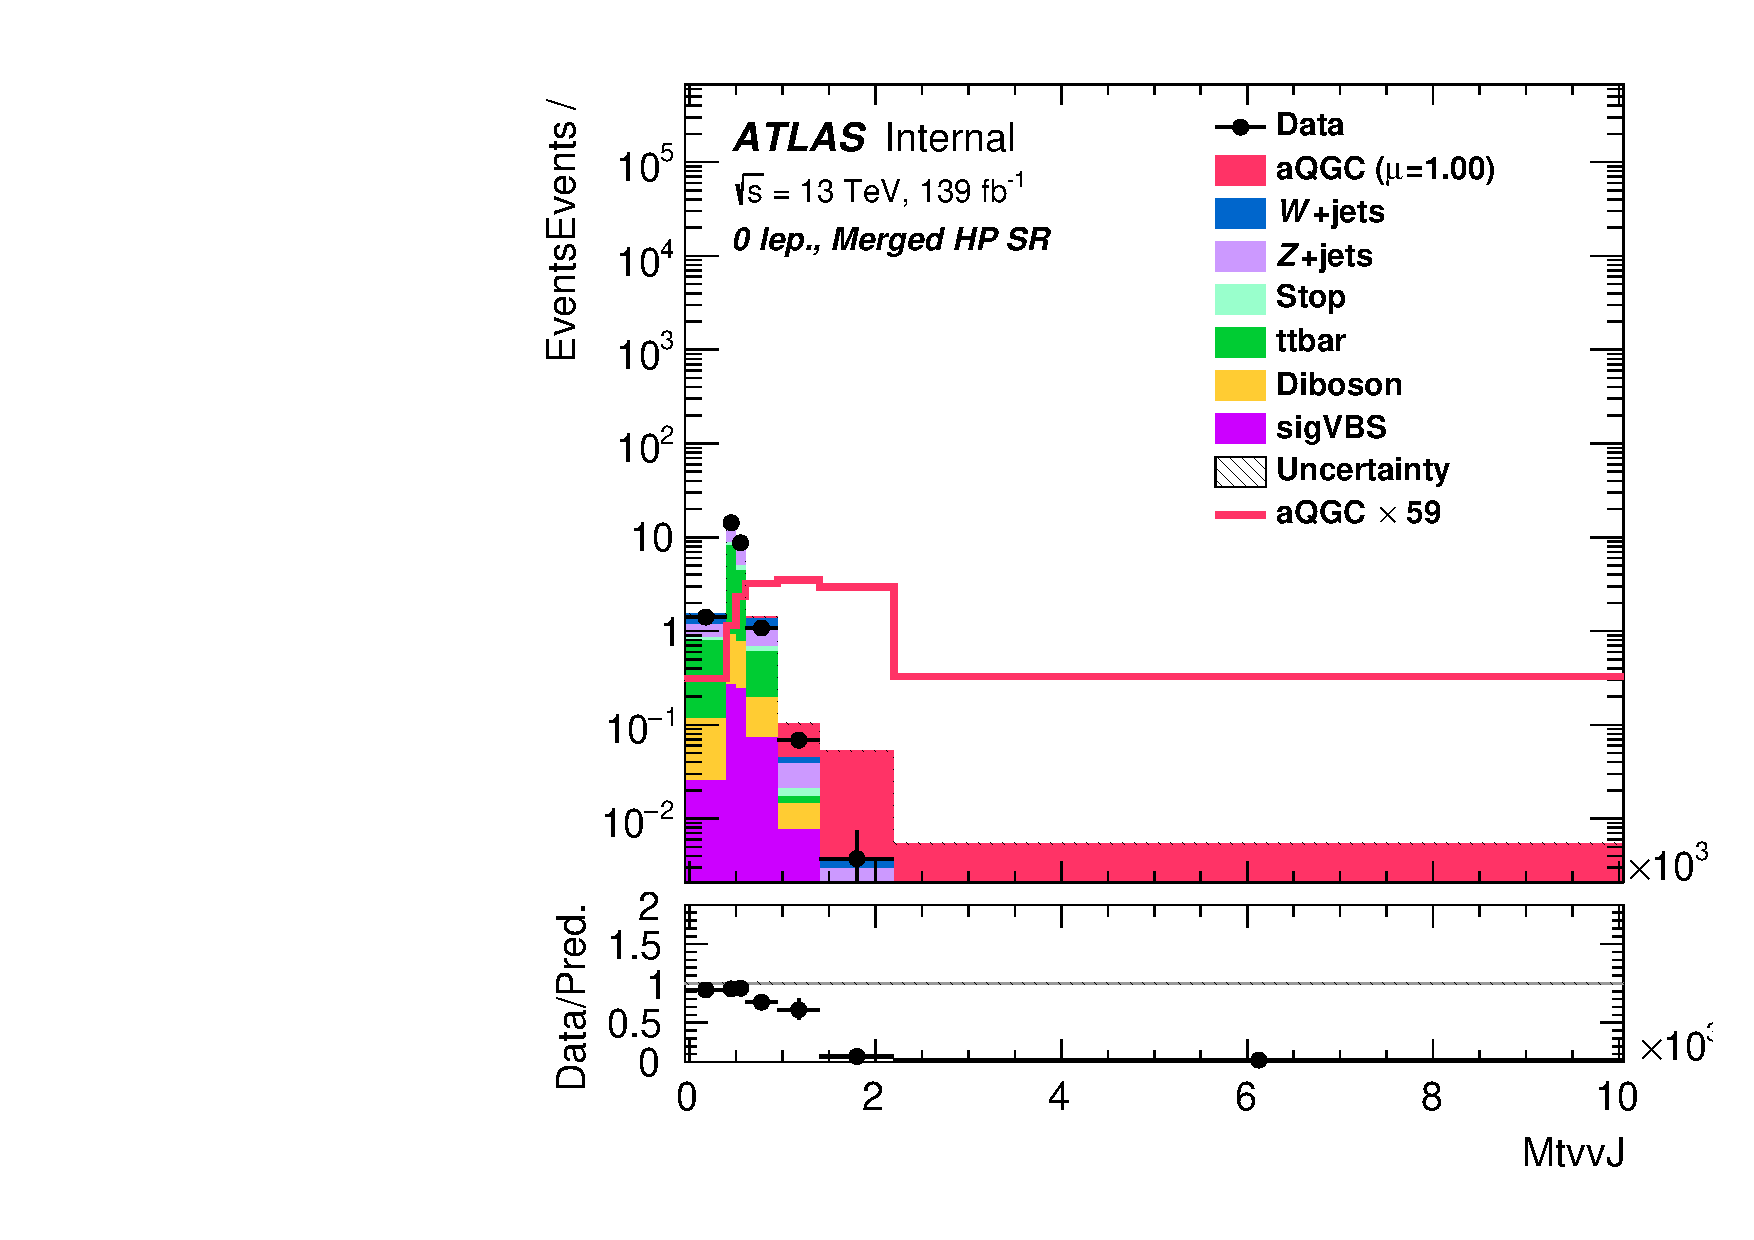
\includegraphics[width=0.32\textwidth]{figures/aQGC/Region_distMtvvJ_DSRVBSHP_BMin0_J0_incJet1_L0_T0_incFat1_Y6051_incTag1_Fat1_Prefitlog.pdf}}
%        \caption{Prefit plots for operator FT0 in \zlep channel are shown. The standard model EW signal is floated as the background.}
%        \label{fig:0lepFT0}
%\end{figure}
%
%\begin{figure}[ht]
%    \centering
%    	\subfigure[ 1lep merged Vjet CR ]{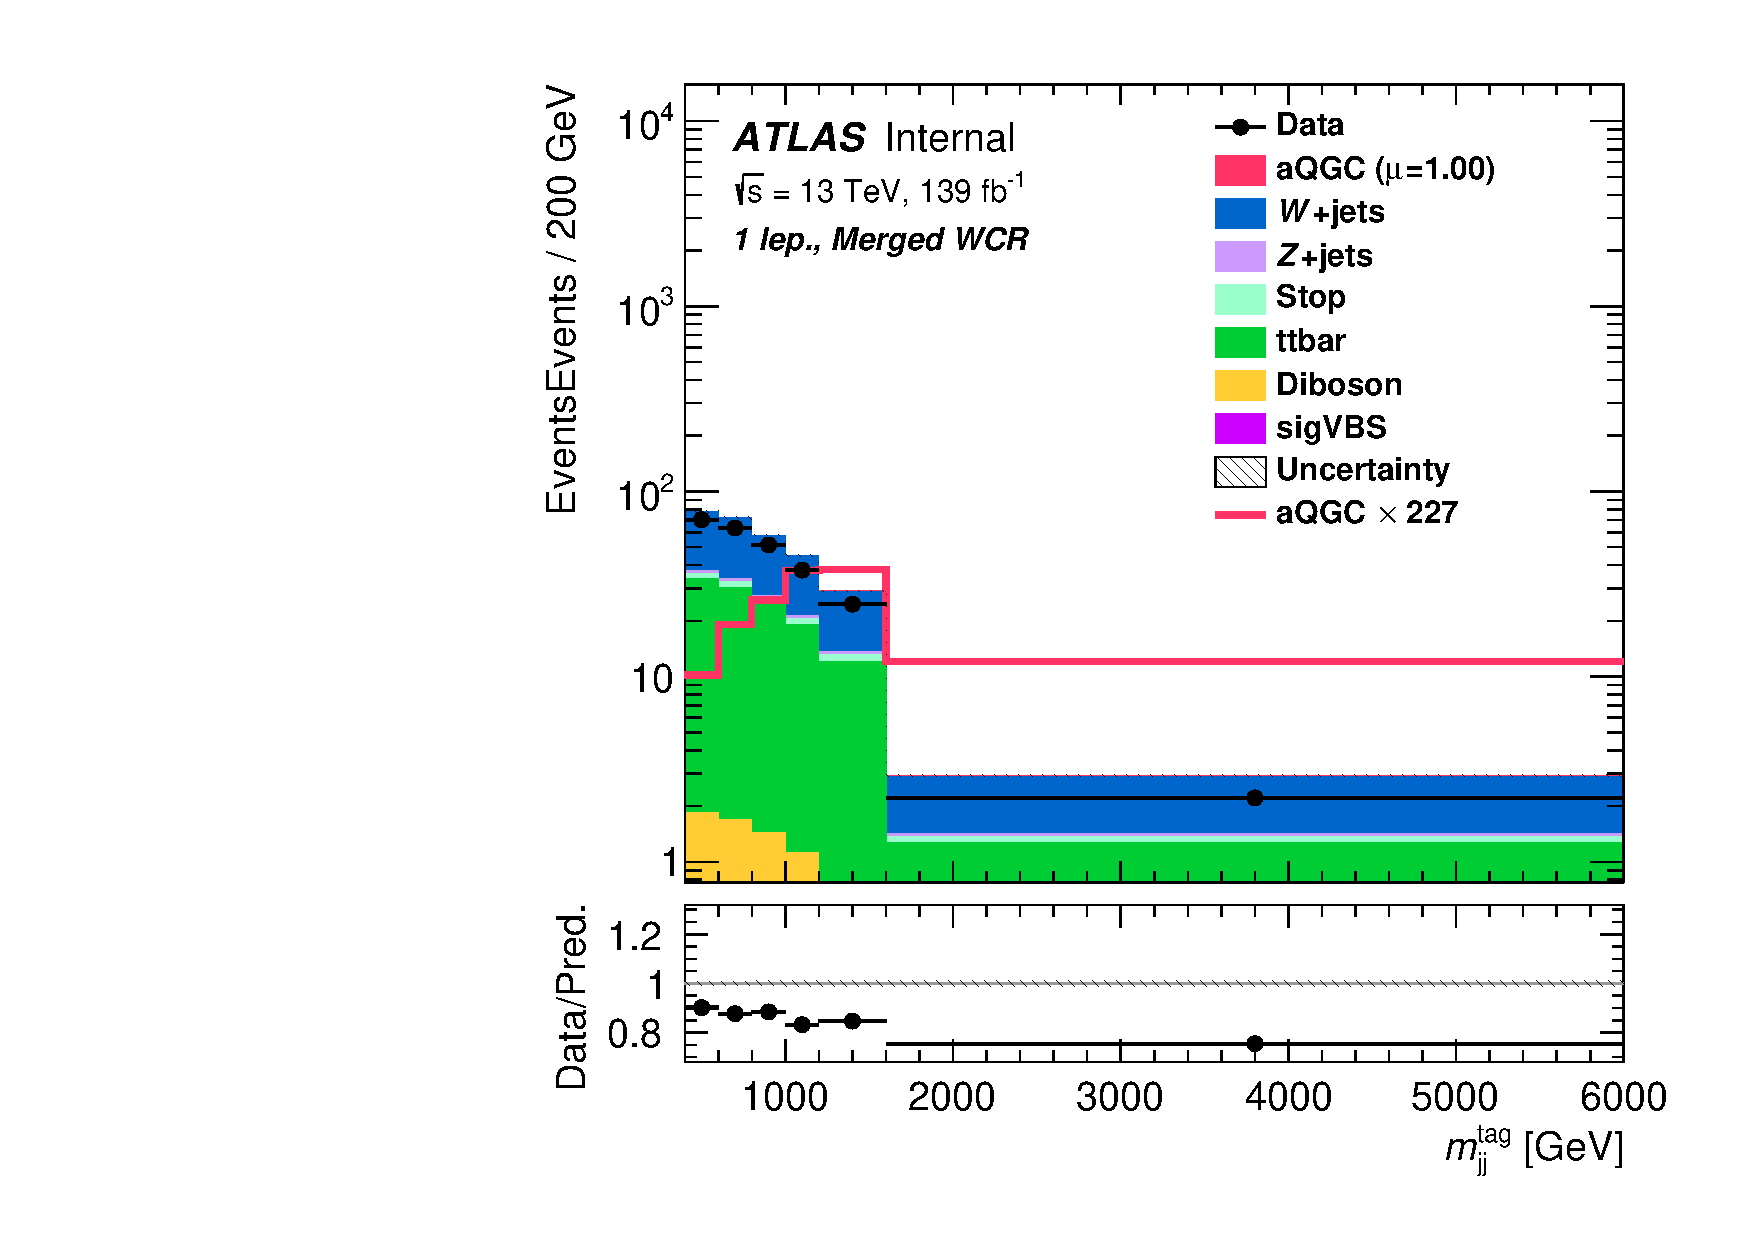
\includegraphics[width=0.32\textwidth]{figures/aQGC/Region_disttagMjj_DCRVjetMerged_BMin0_J0_incJet1_L1_T0_incFat1_Y6051_incTag1_Fat1_Prefitlog.pdf}}
%    	\subfigure[ 1lep HP Top CR ]{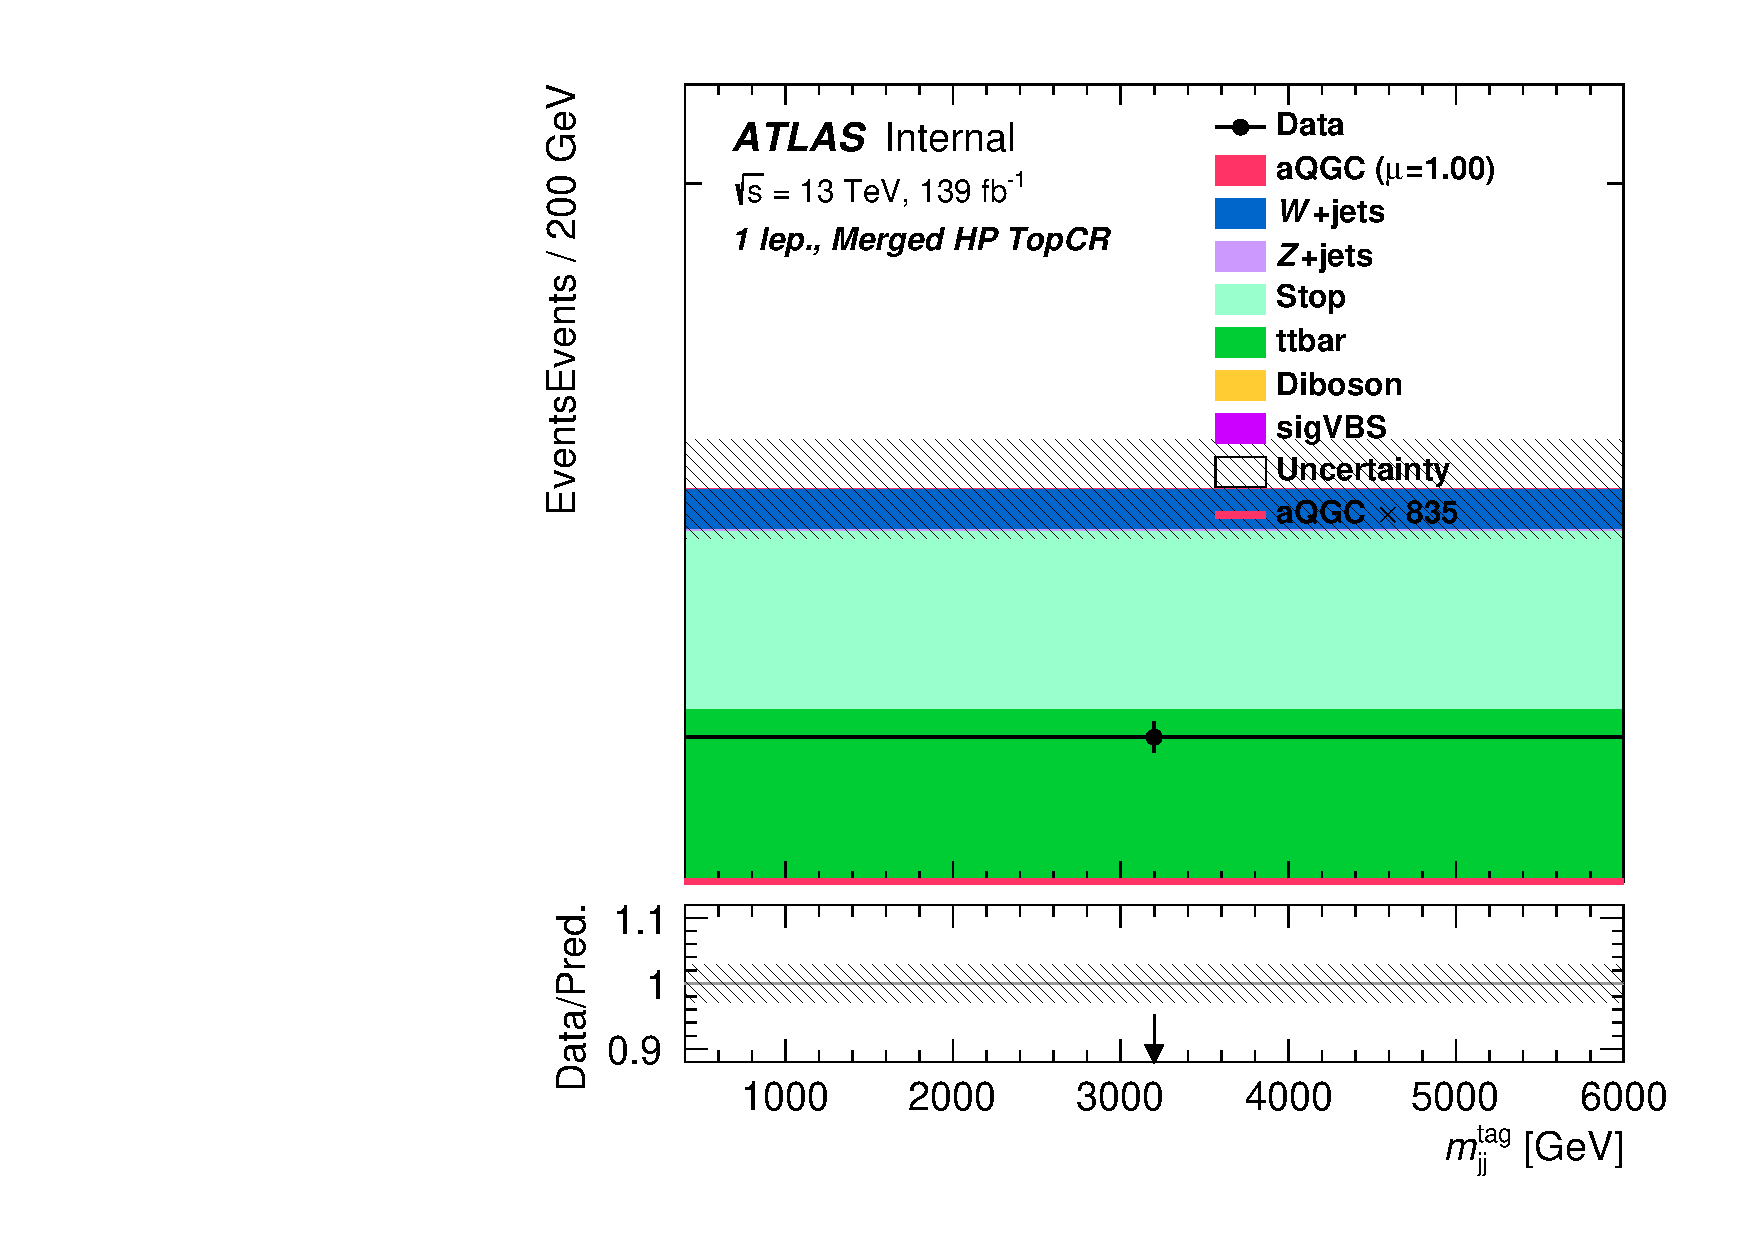
\includegraphics[width=0.32\textwidth]{figures/aQGC/Region_disttagMjj_DCRTopHP_BMin0_J0_incJet1_L1_T0_incFat1_Y6051_incTag1_Fat1_Prefitlog.pdf}}
%    	\subfigure[ 1lep LP Top CR ]{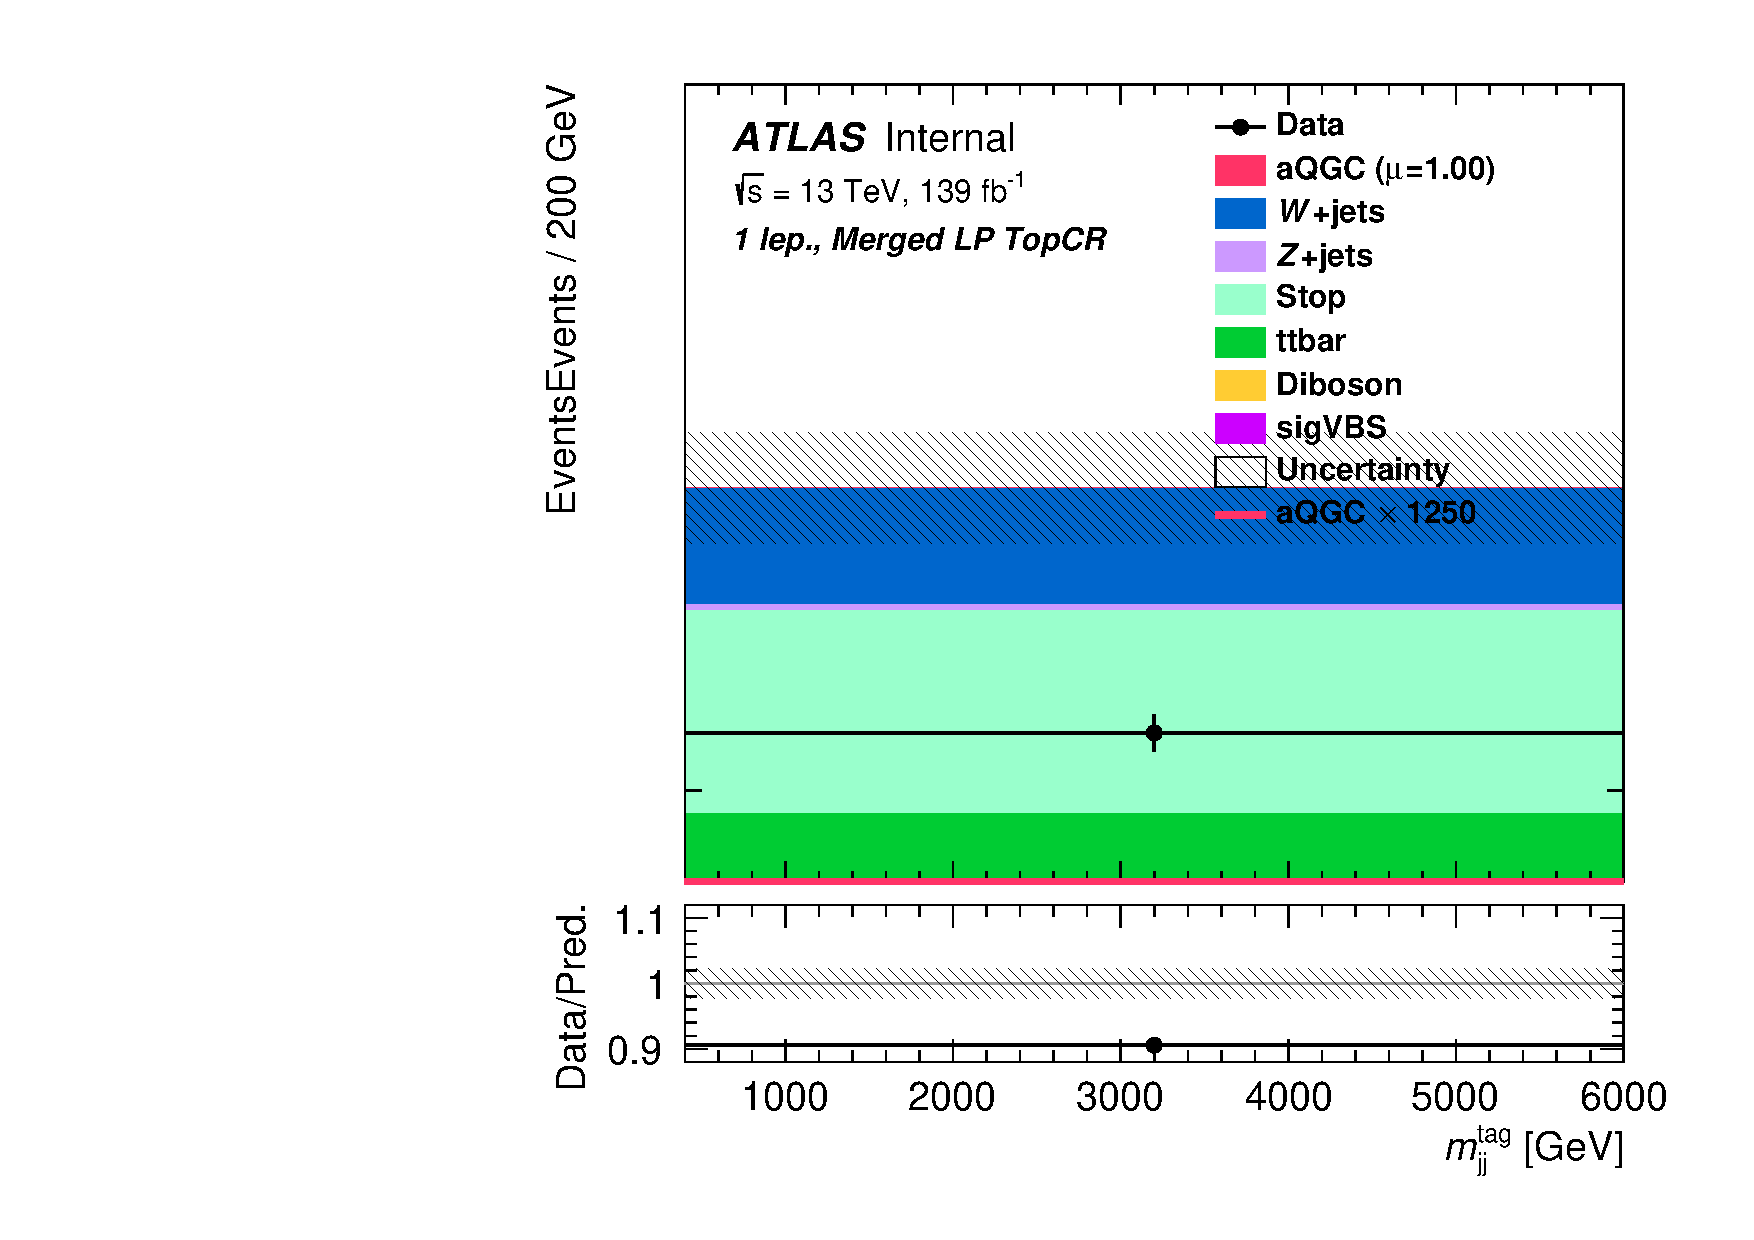
\includegraphics[width=0.32\textwidth]{figures/aQGC/Region_disttagMjj_DCRTopLP_BMin0_J0_incJet1_L1_T0_incFat1_Y6051_incTag1_Fat1_Prefitlog.pdf}}
%    	\subfigure[ 1lep HP SR ]{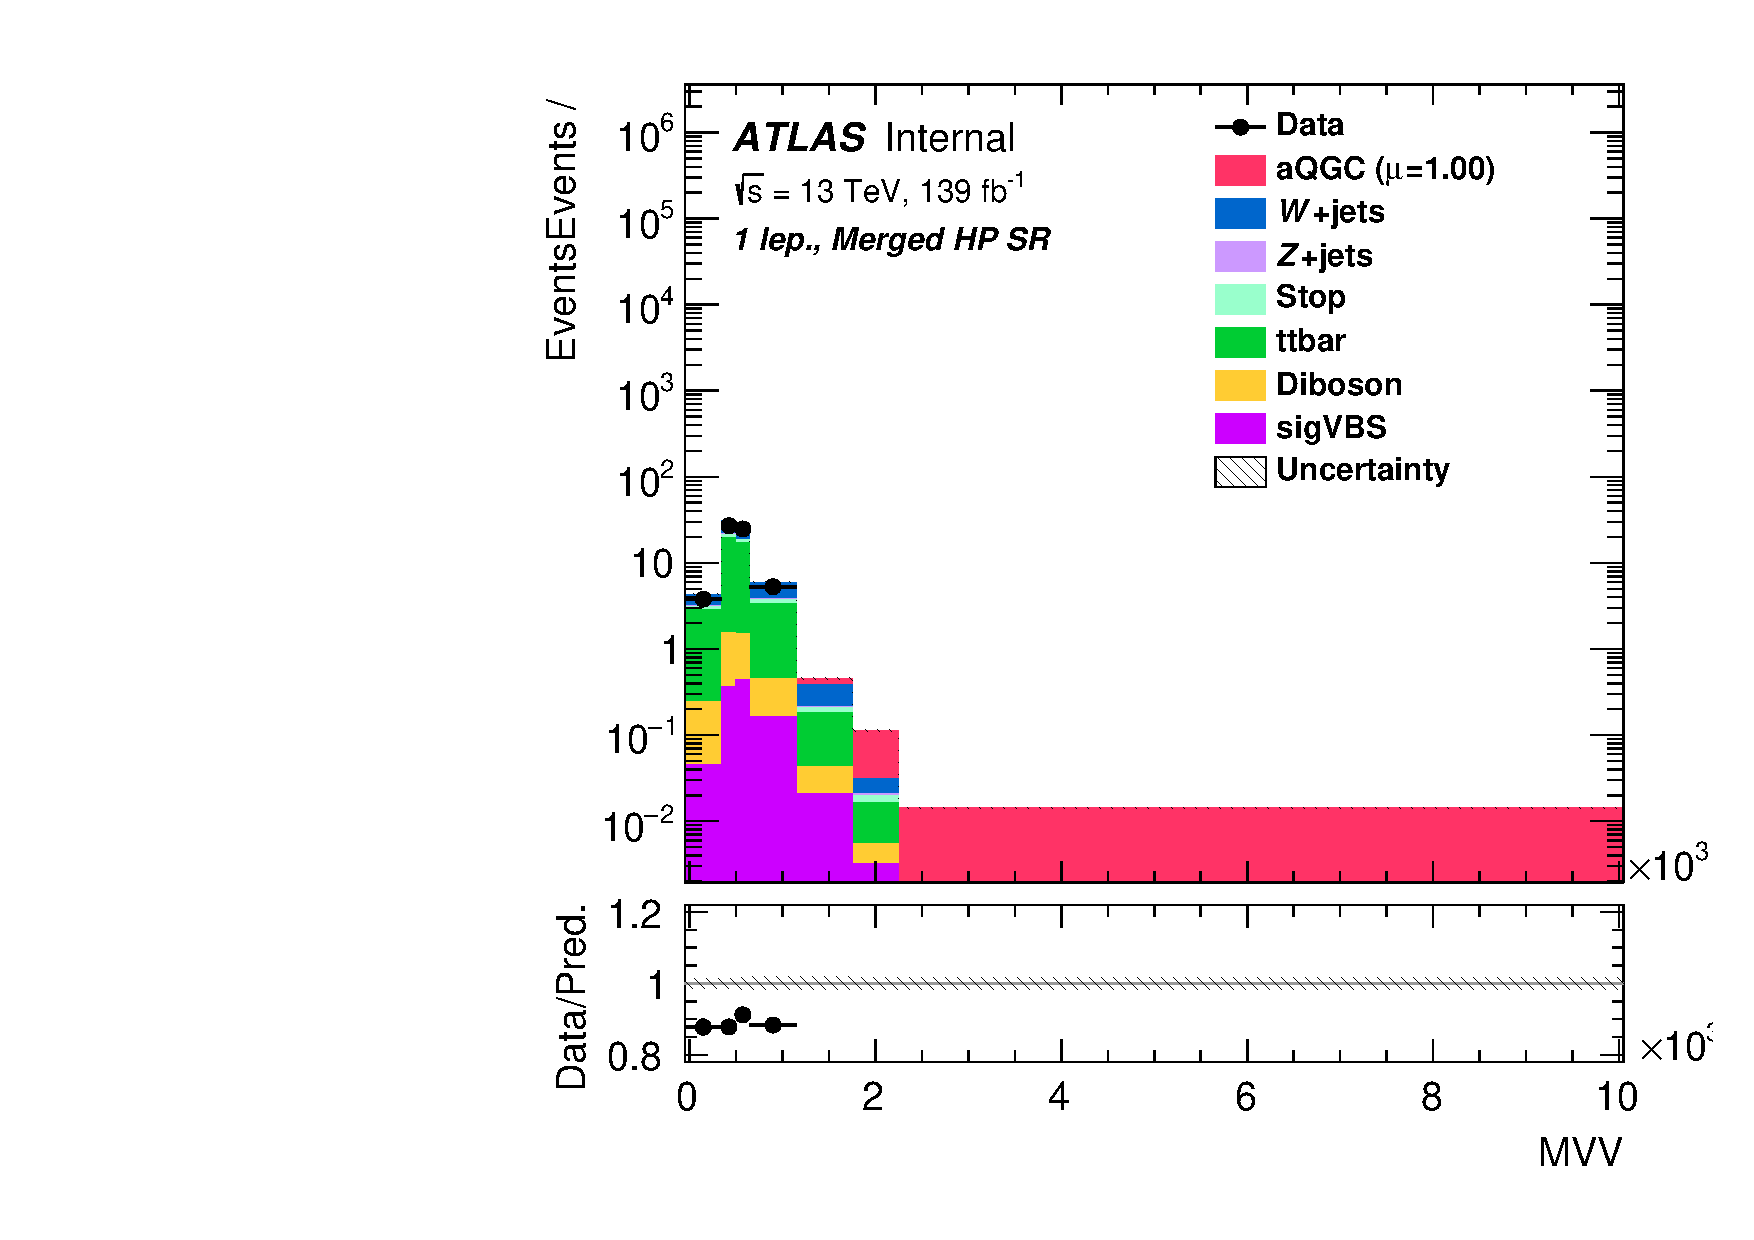
\includegraphics[width=0.32\textwidth]{figures/aQGC/Region_distMVV_DSRVBSHP_BMin0_J0_incJet1_L1_T0_incFat1_Y6051_incTag1_Fat1_Prefitlog.pdf}}
%    	\subfigure[ 1lep LP SR ]{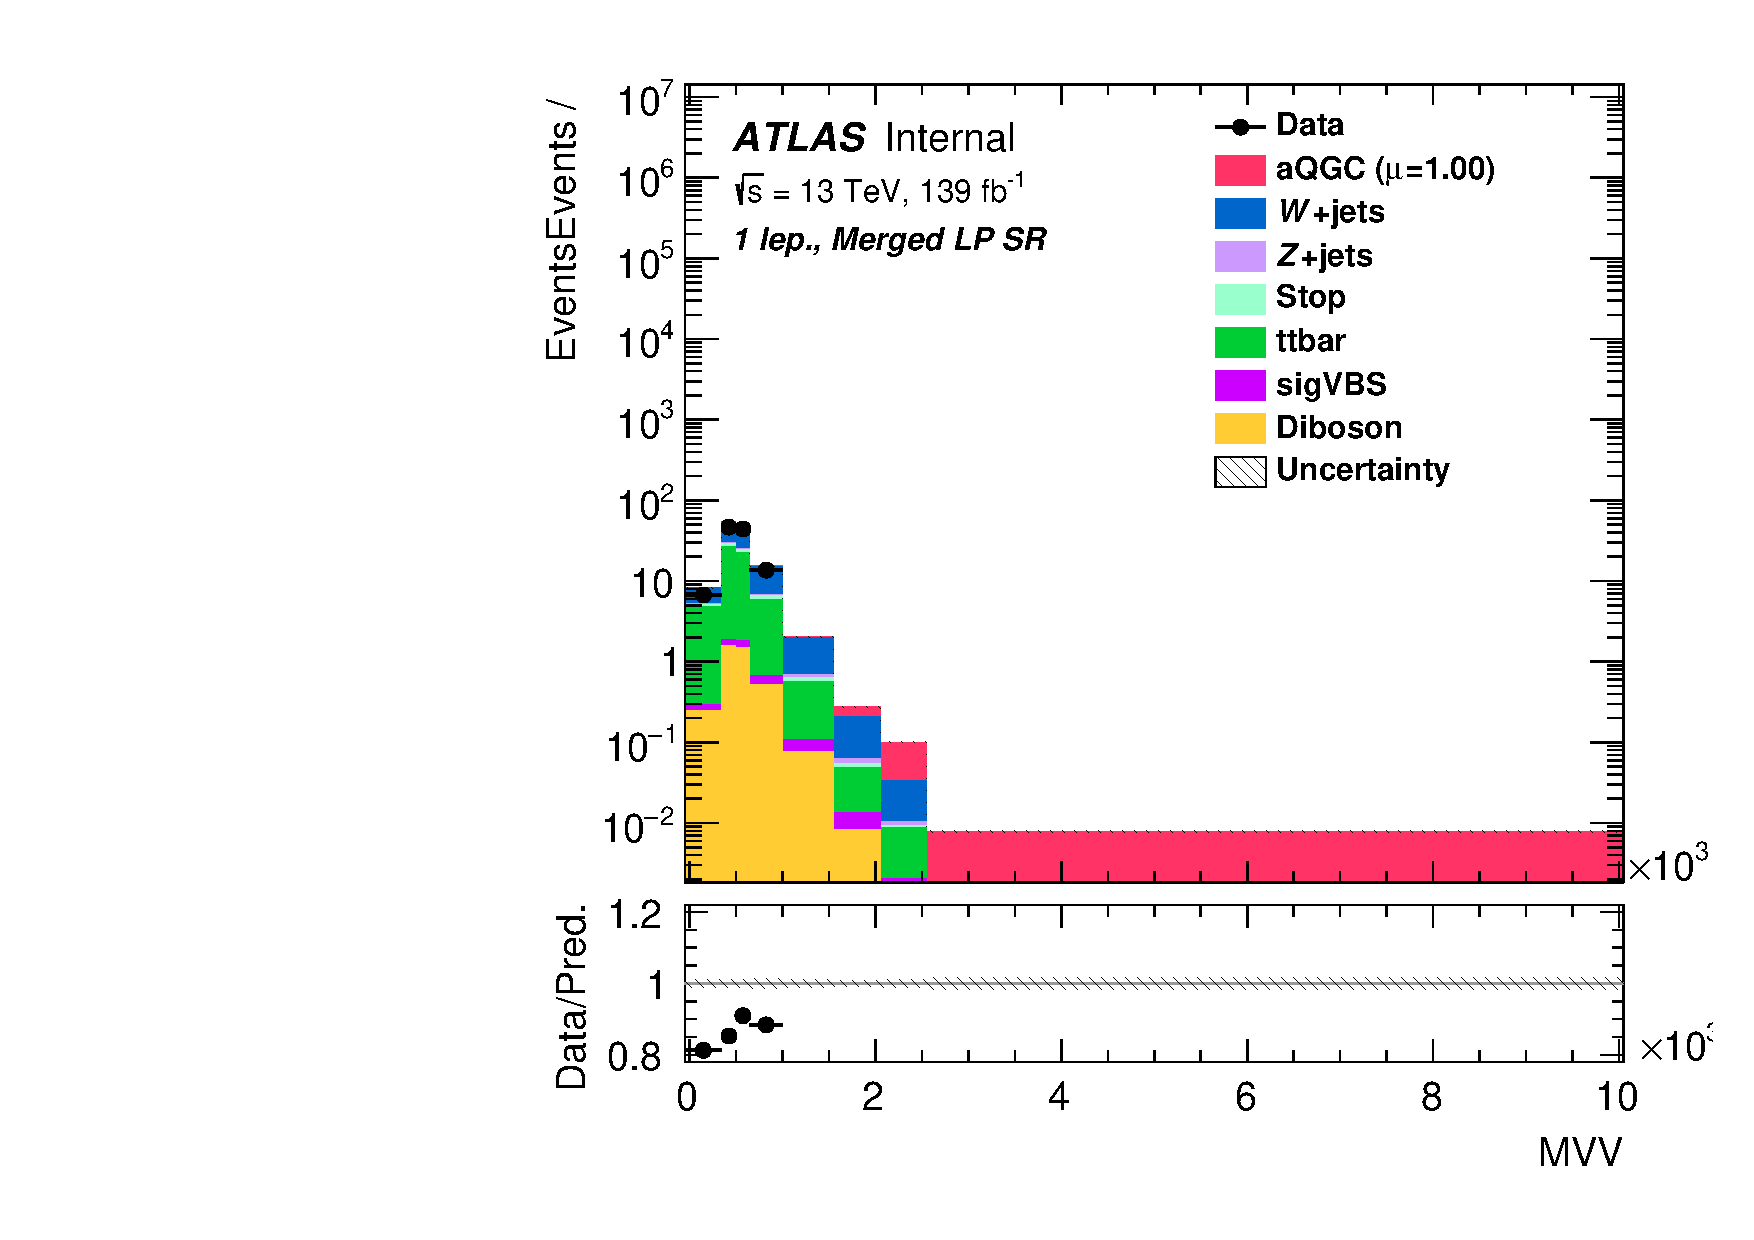
\includegraphics[width=0.32\textwidth]{figures/aQGC/Region_distMVV_DSRVBSLP_BMin0_J0_incJet1_L1_T0_incFat1_Y6051_incTag1_Fat1_Prefitlog.pdf}}
%    	\subfigure[ 1lep resolved Vjet CR ]{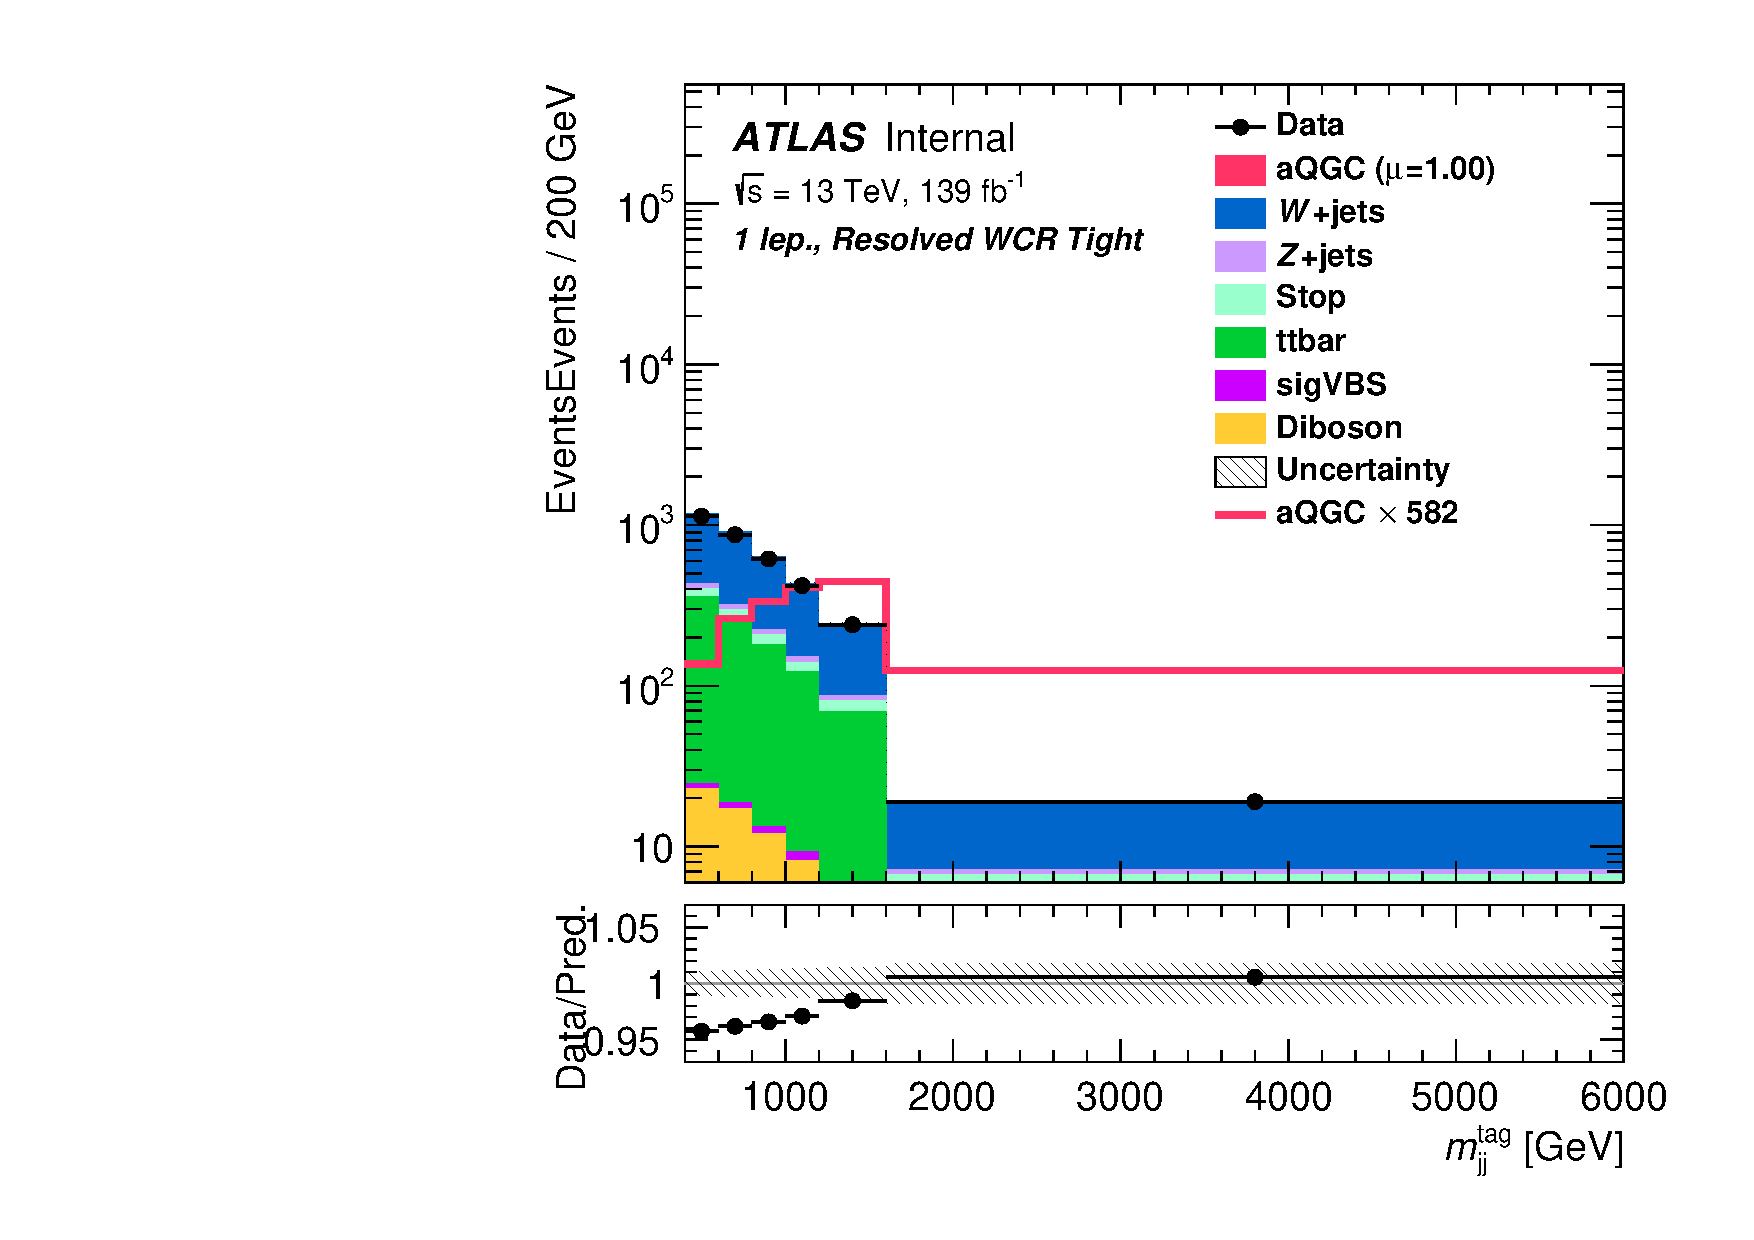
\includegraphics[width=0.32\textwidth]{figures/aQGC/Region_disttagMjj_DCRVjetTight_BMin0_T0_Y6051_incTag1_J2_L1_incJet1_Prefitlog.pdf}}
%    	\subfigure[ 1lep resolved Top CR ]{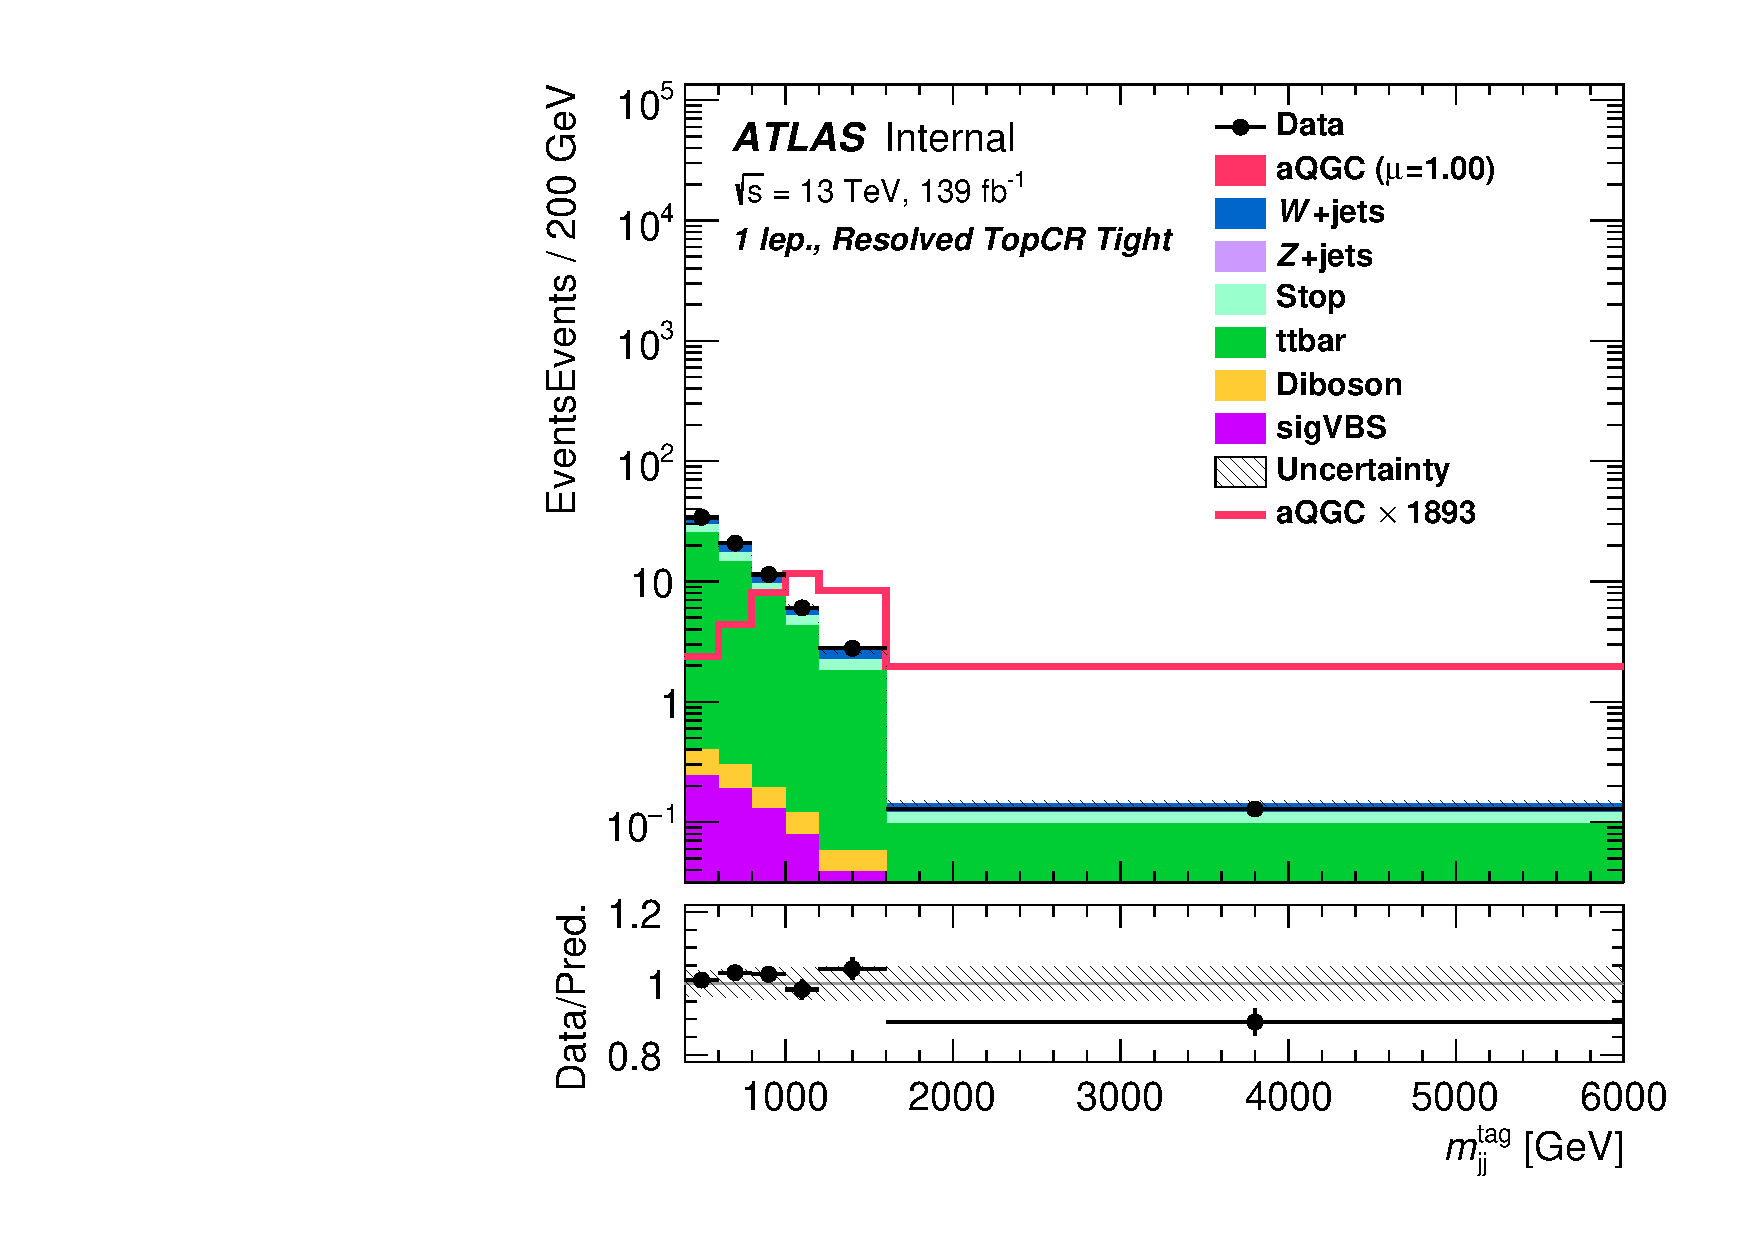
\includegraphics[width=0.32\textwidth]{figures/aQGC/Region_disttagMjj_DCRTopTight_BMin0_T0_Y6051_incTag1_J2_L1_incJet1_Prefitlog.pdf}}
%    	\subfigure[ 1lep resolved SR ]{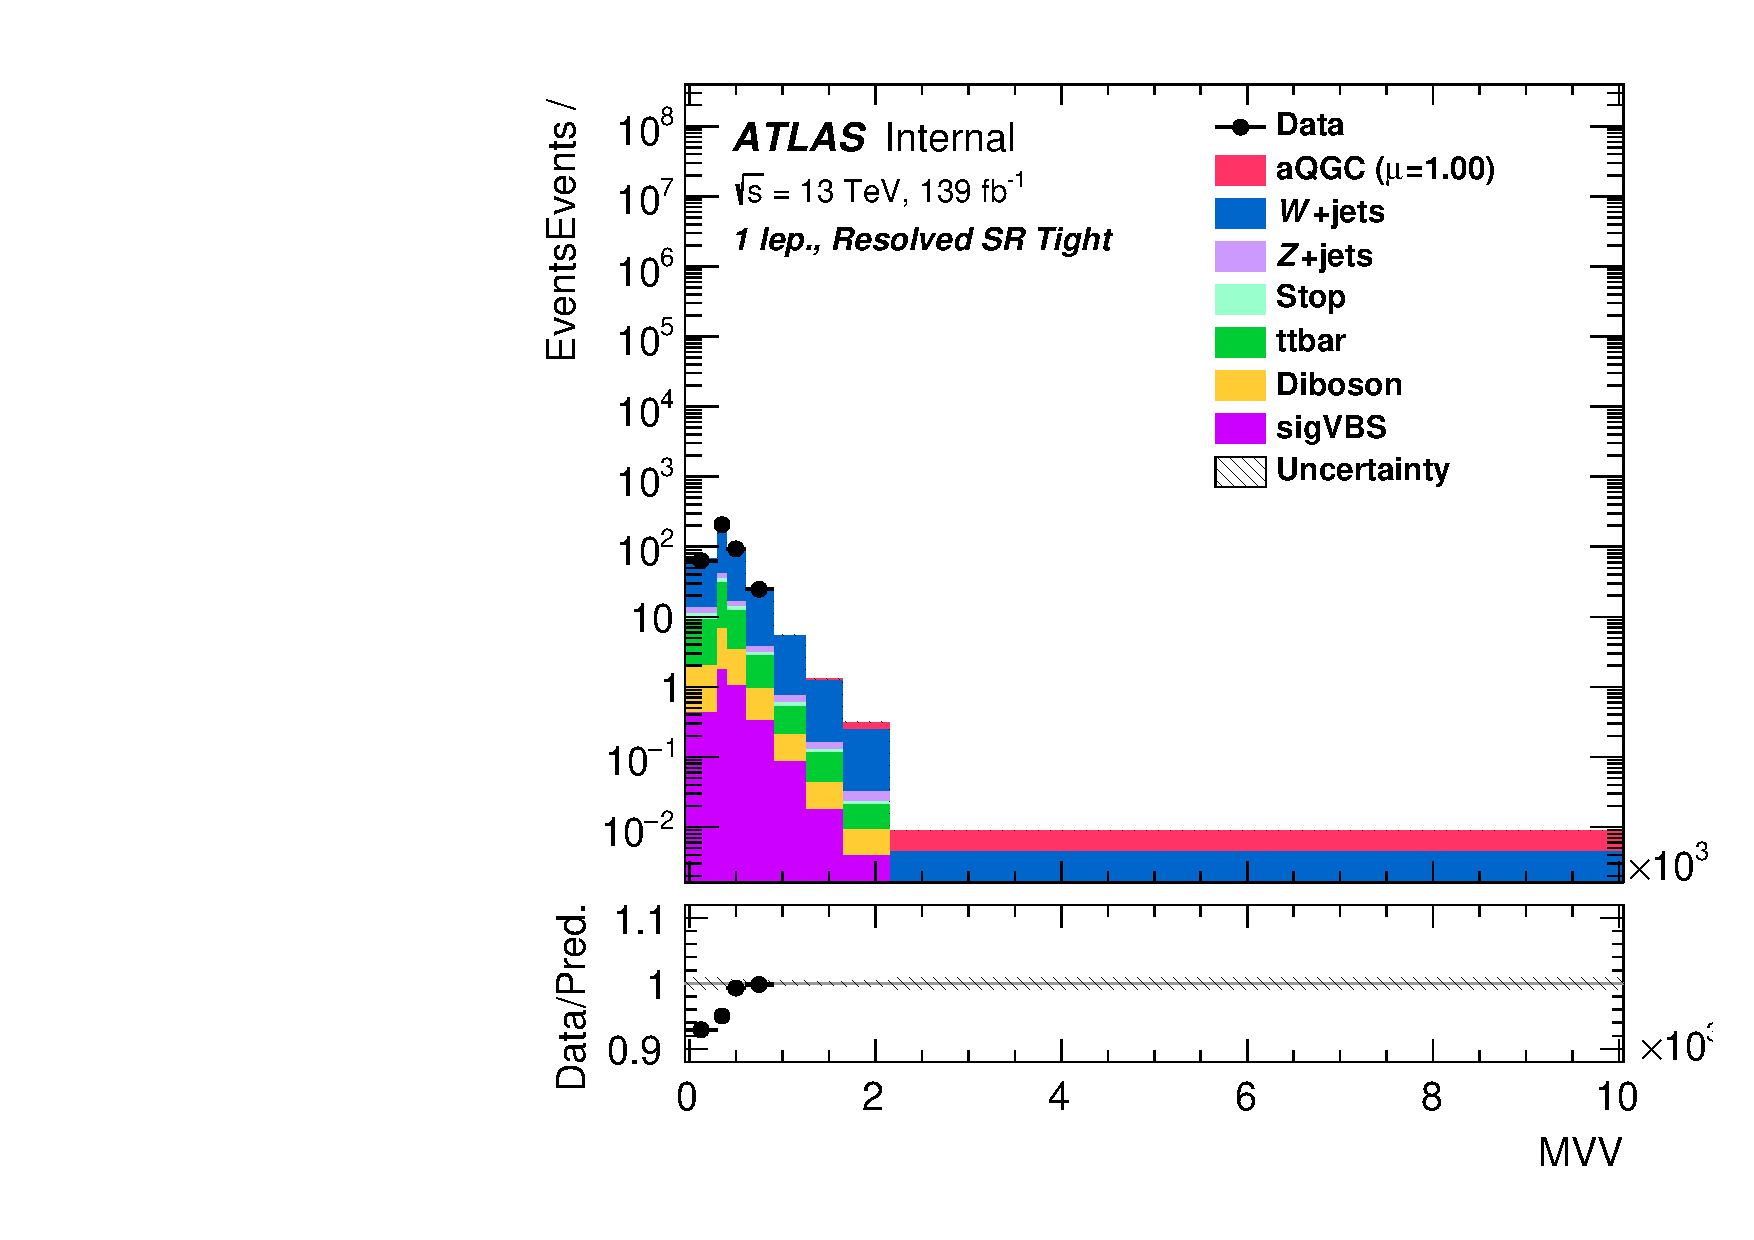
\includegraphics[width=0.32\textwidth]{figures/aQGC/Region_distMVV_DSRVBSTight_BMin0_T0_Y6051_incTag1_J2_L1_incJet1_Prefitlog.pdf}}
%        \caption{Prefit plots for operator FT0 in \olep channel are shown. The standard model EW signal is floated as the background.}
%        \label{fig:1lepFT0}
%\end{figure}
%
%\begin{figure}[ht]
%    \centering
%    	\subfigure[ 2lep merged CR ]{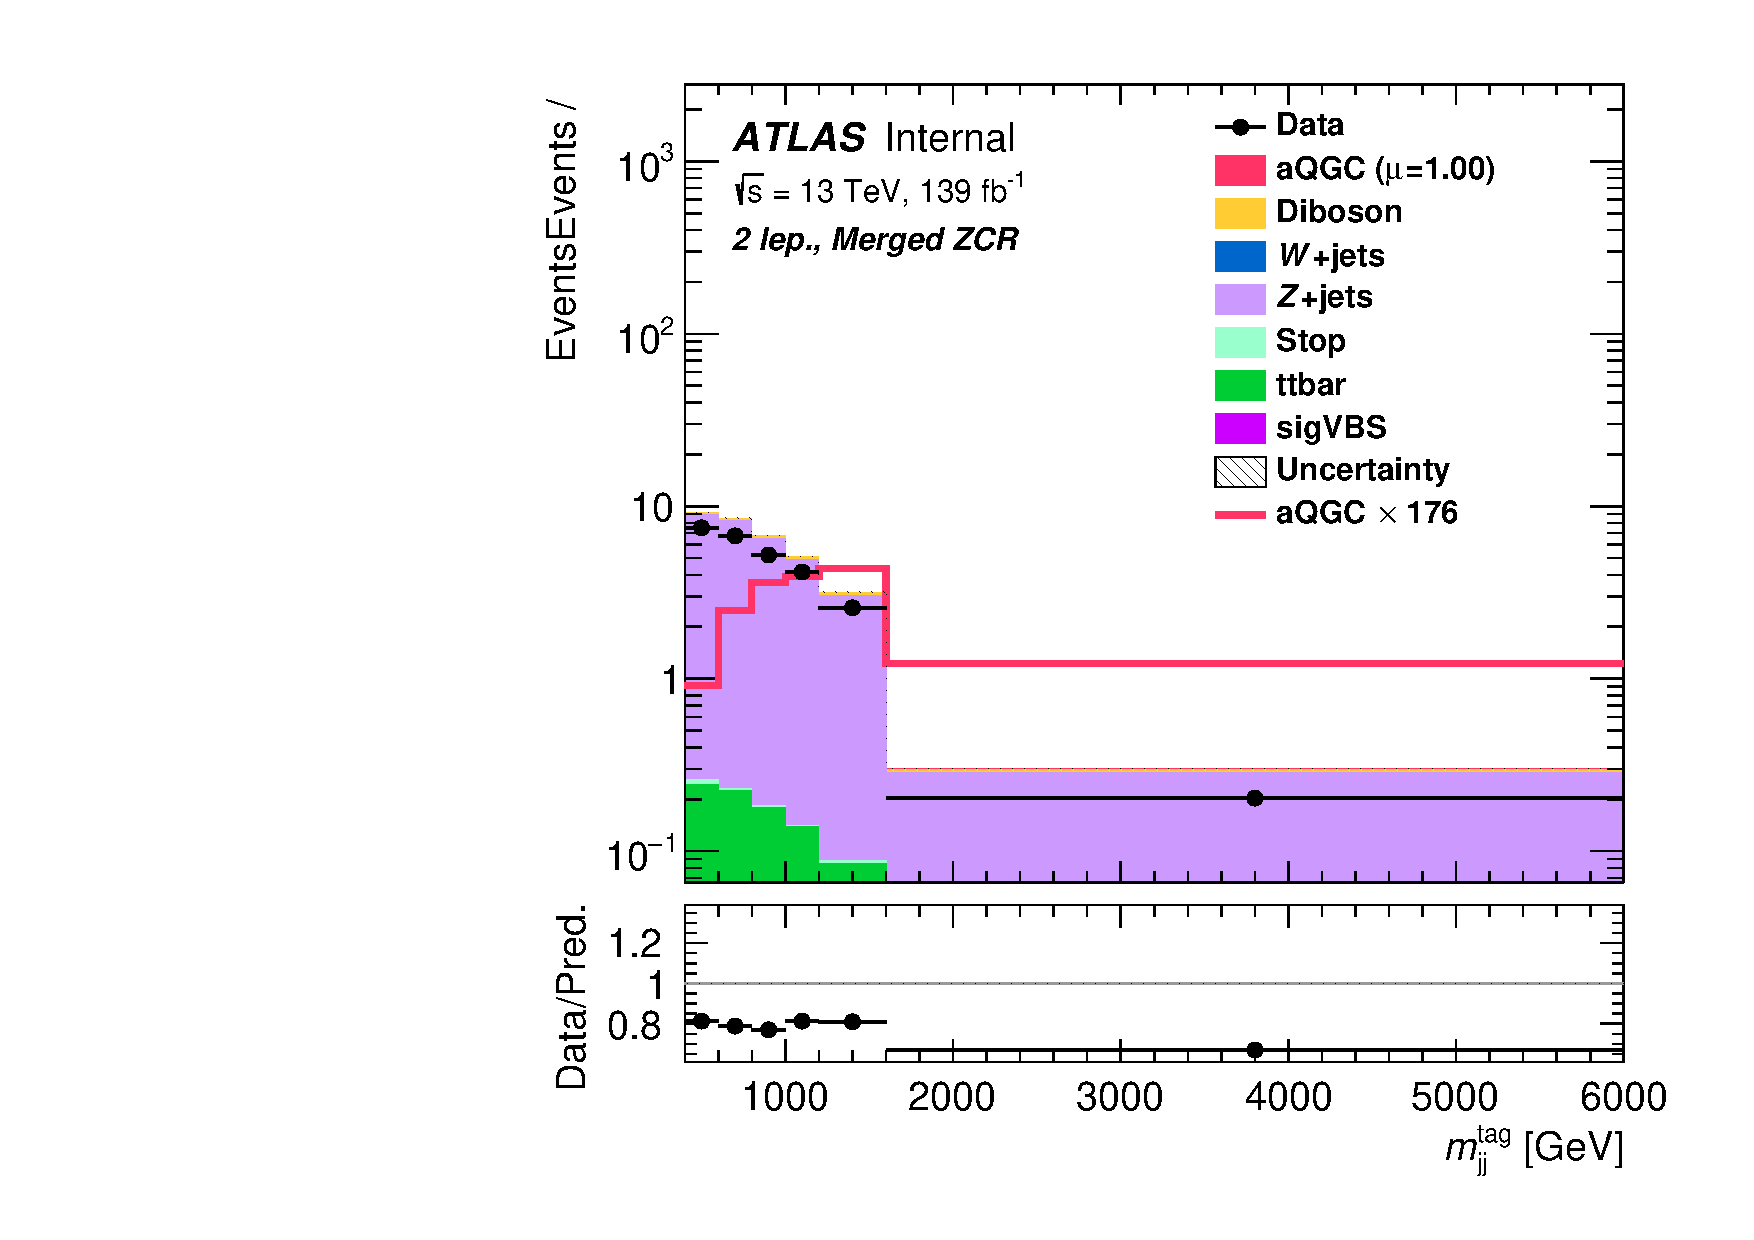
\includegraphics[width=0.32\textwidth]{figures/aQGC/Region_distMTagMerJets_DCRVjet_BMin0_J0_incJet1_L2_T0_incFat1_Y6051_incTag1_Fat1_Prefitlog.pdf}}
%    	\subfigure[ 2lep HP SR ]{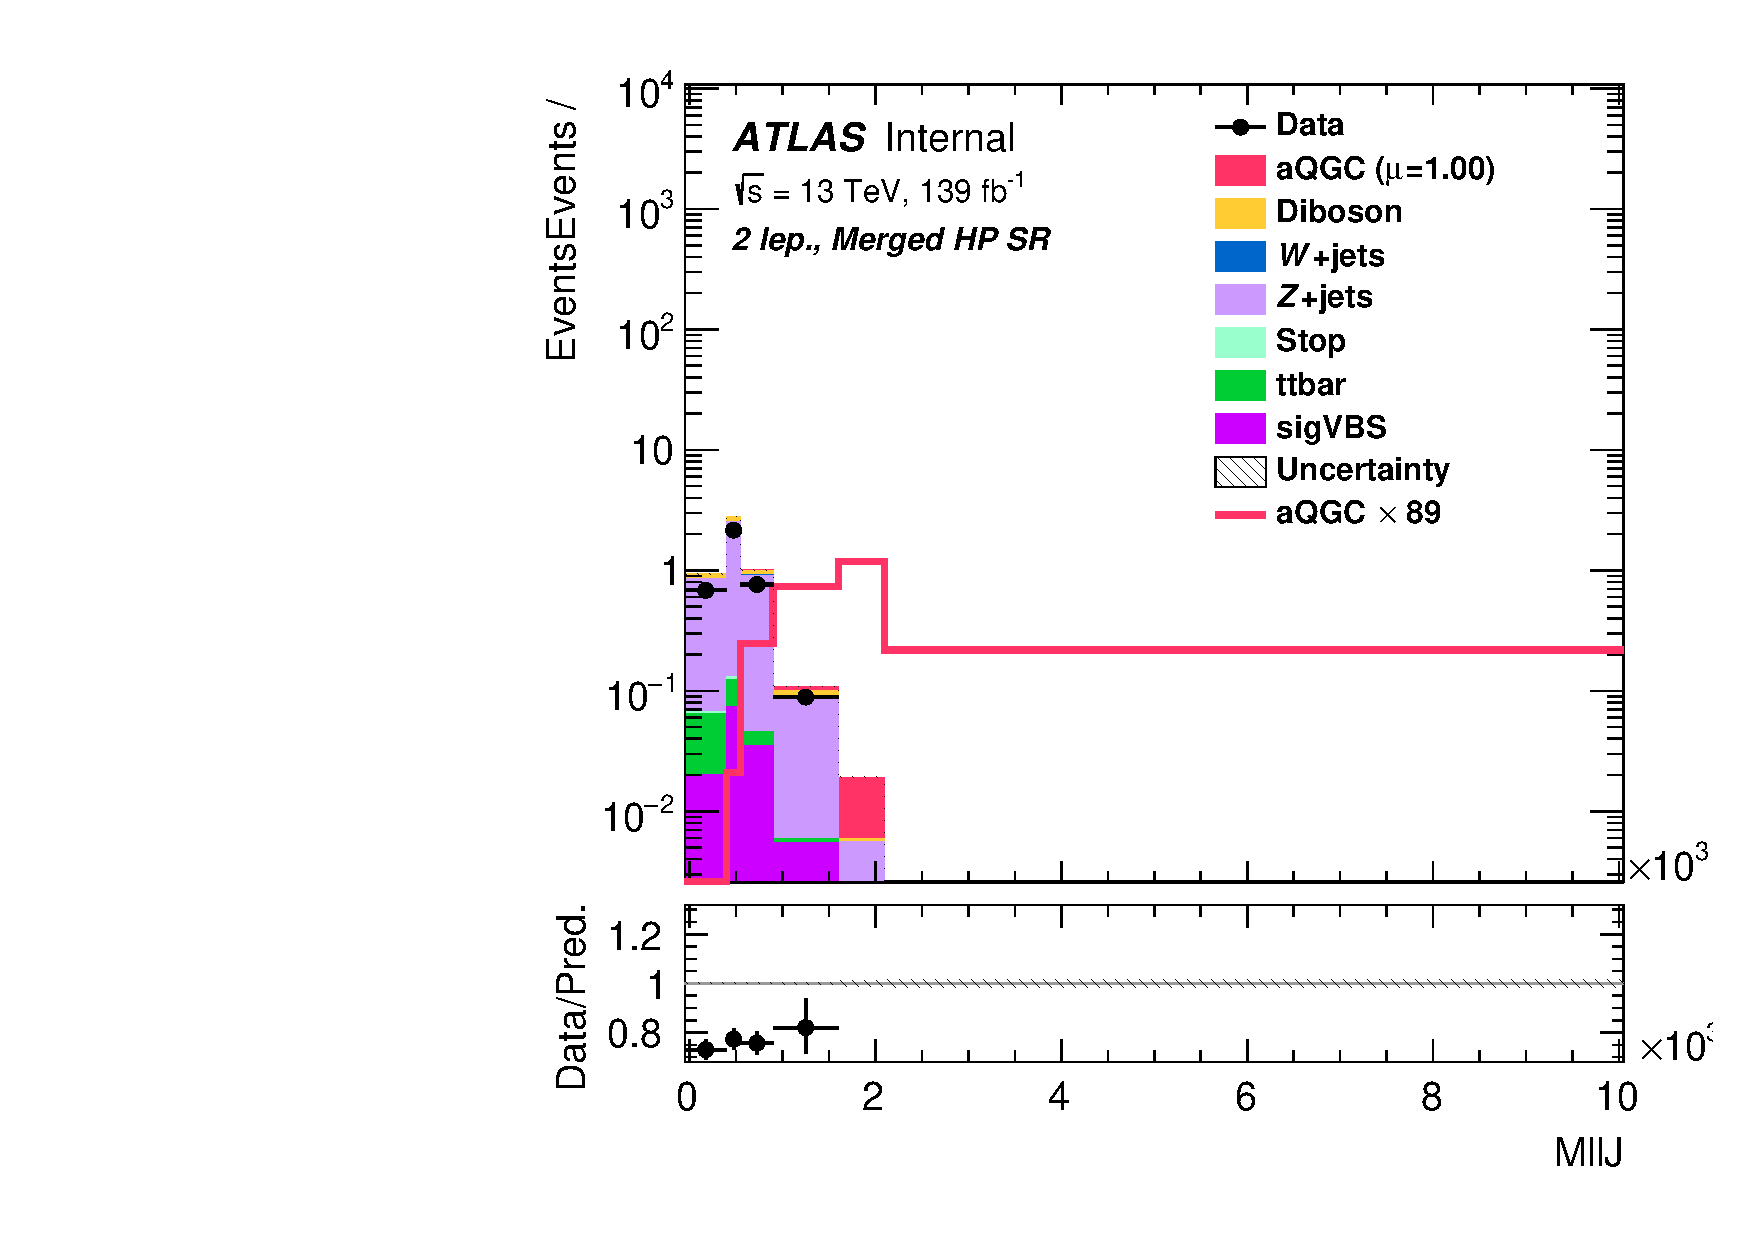
\includegraphics[width=0.32\textwidth]{figures/aQGC/Region_distMllJ_DSRVBSHP_BMin0_J0_incJet1_L2_T0_incFat1_Y6051_incTag1_Fat1_Prefitlog.pdf}}
%    	\subfigure[ 2lep LP SR ]{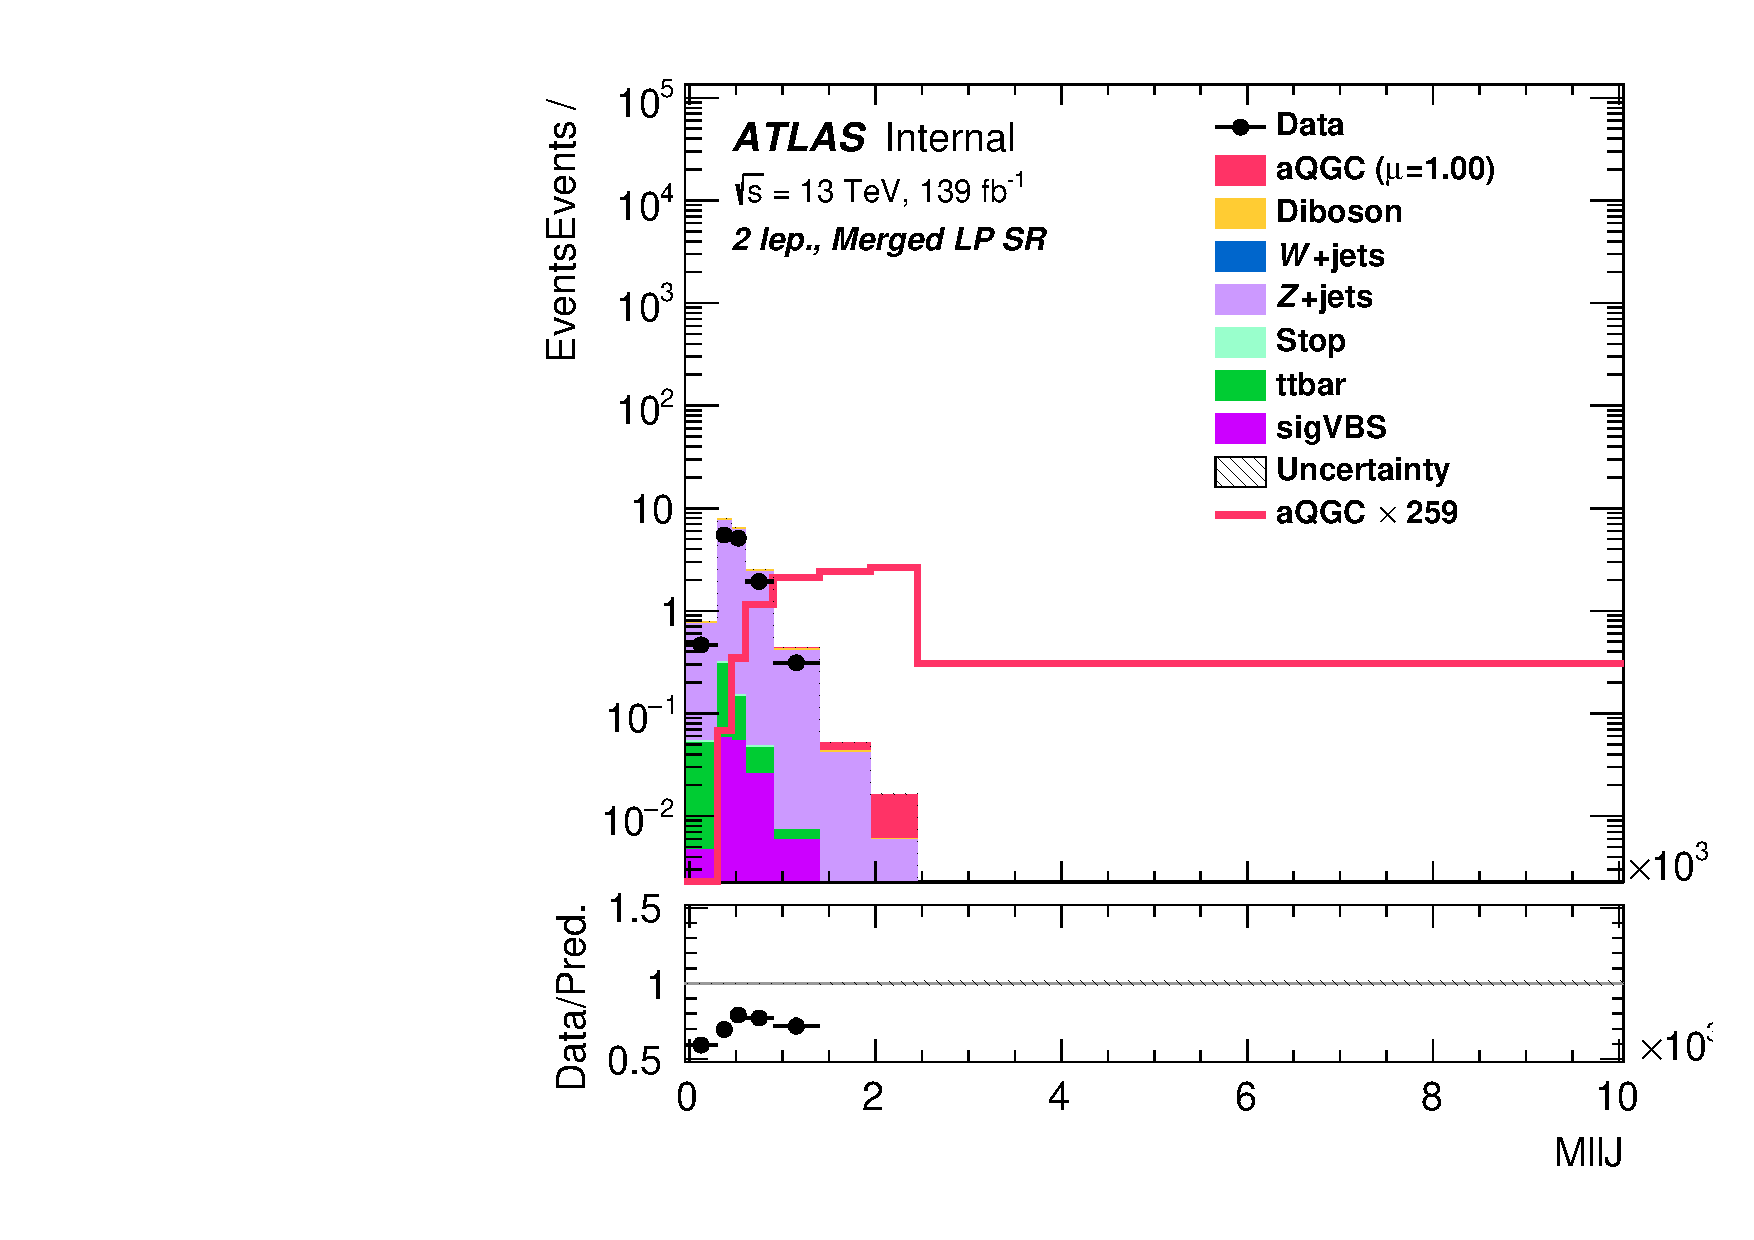
\includegraphics[width=0.32\textwidth]{figures/aQGC/Region_distMllJ_DSRVBSLP_BMin0_J0_incJet1_L2_T0_incFat1_Y6051_incTag1_Fat1_Prefitlog.pdf}}
%    	\subfigure[ 2lep resolved CR ]{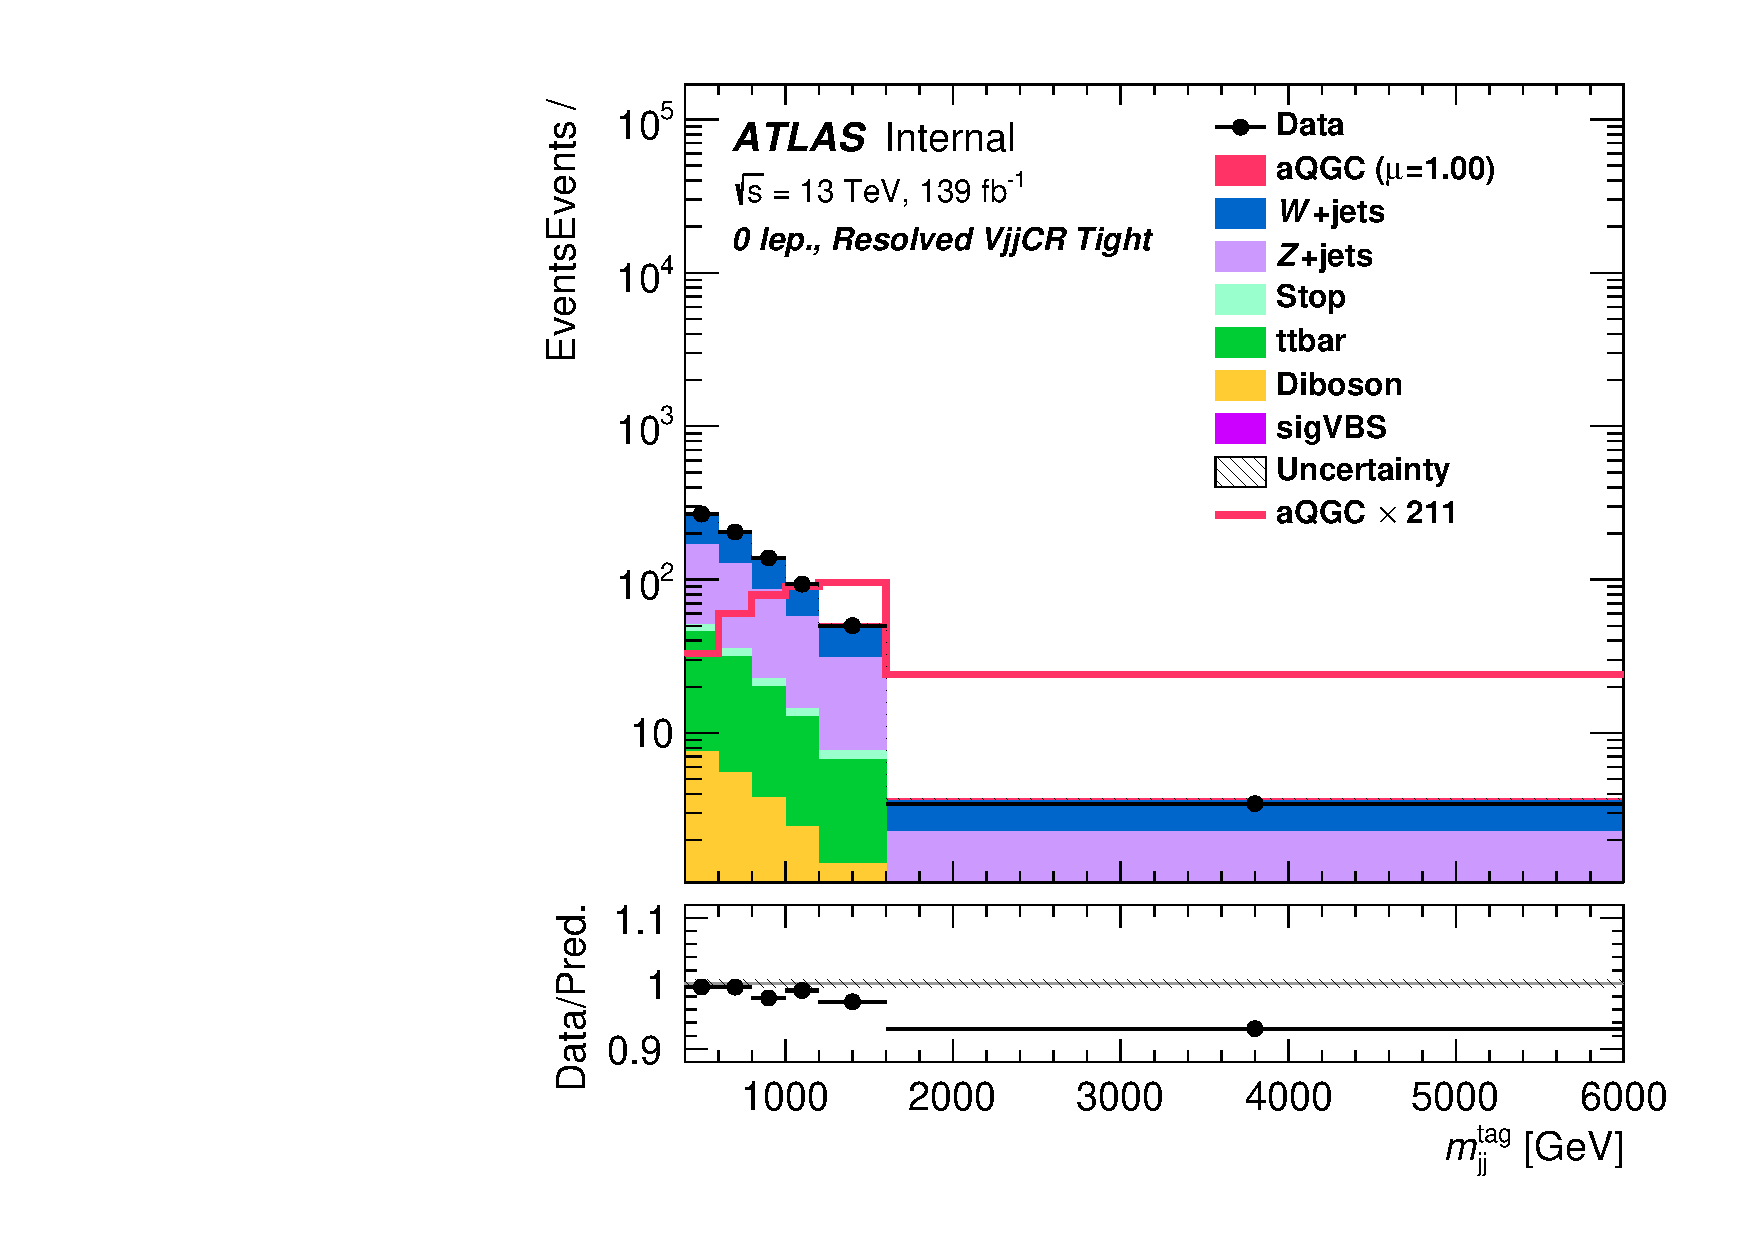
\includegraphics[width=0.32\textwidth]{figures/aQGC/Region_distMTagJets_DCRVjetFid_BMin0_T0_Y6051_incTag1_J2_L0_incJet1_Prefitlog.pdf}}
%    	\subfigure[ 2lep resolved SR ]{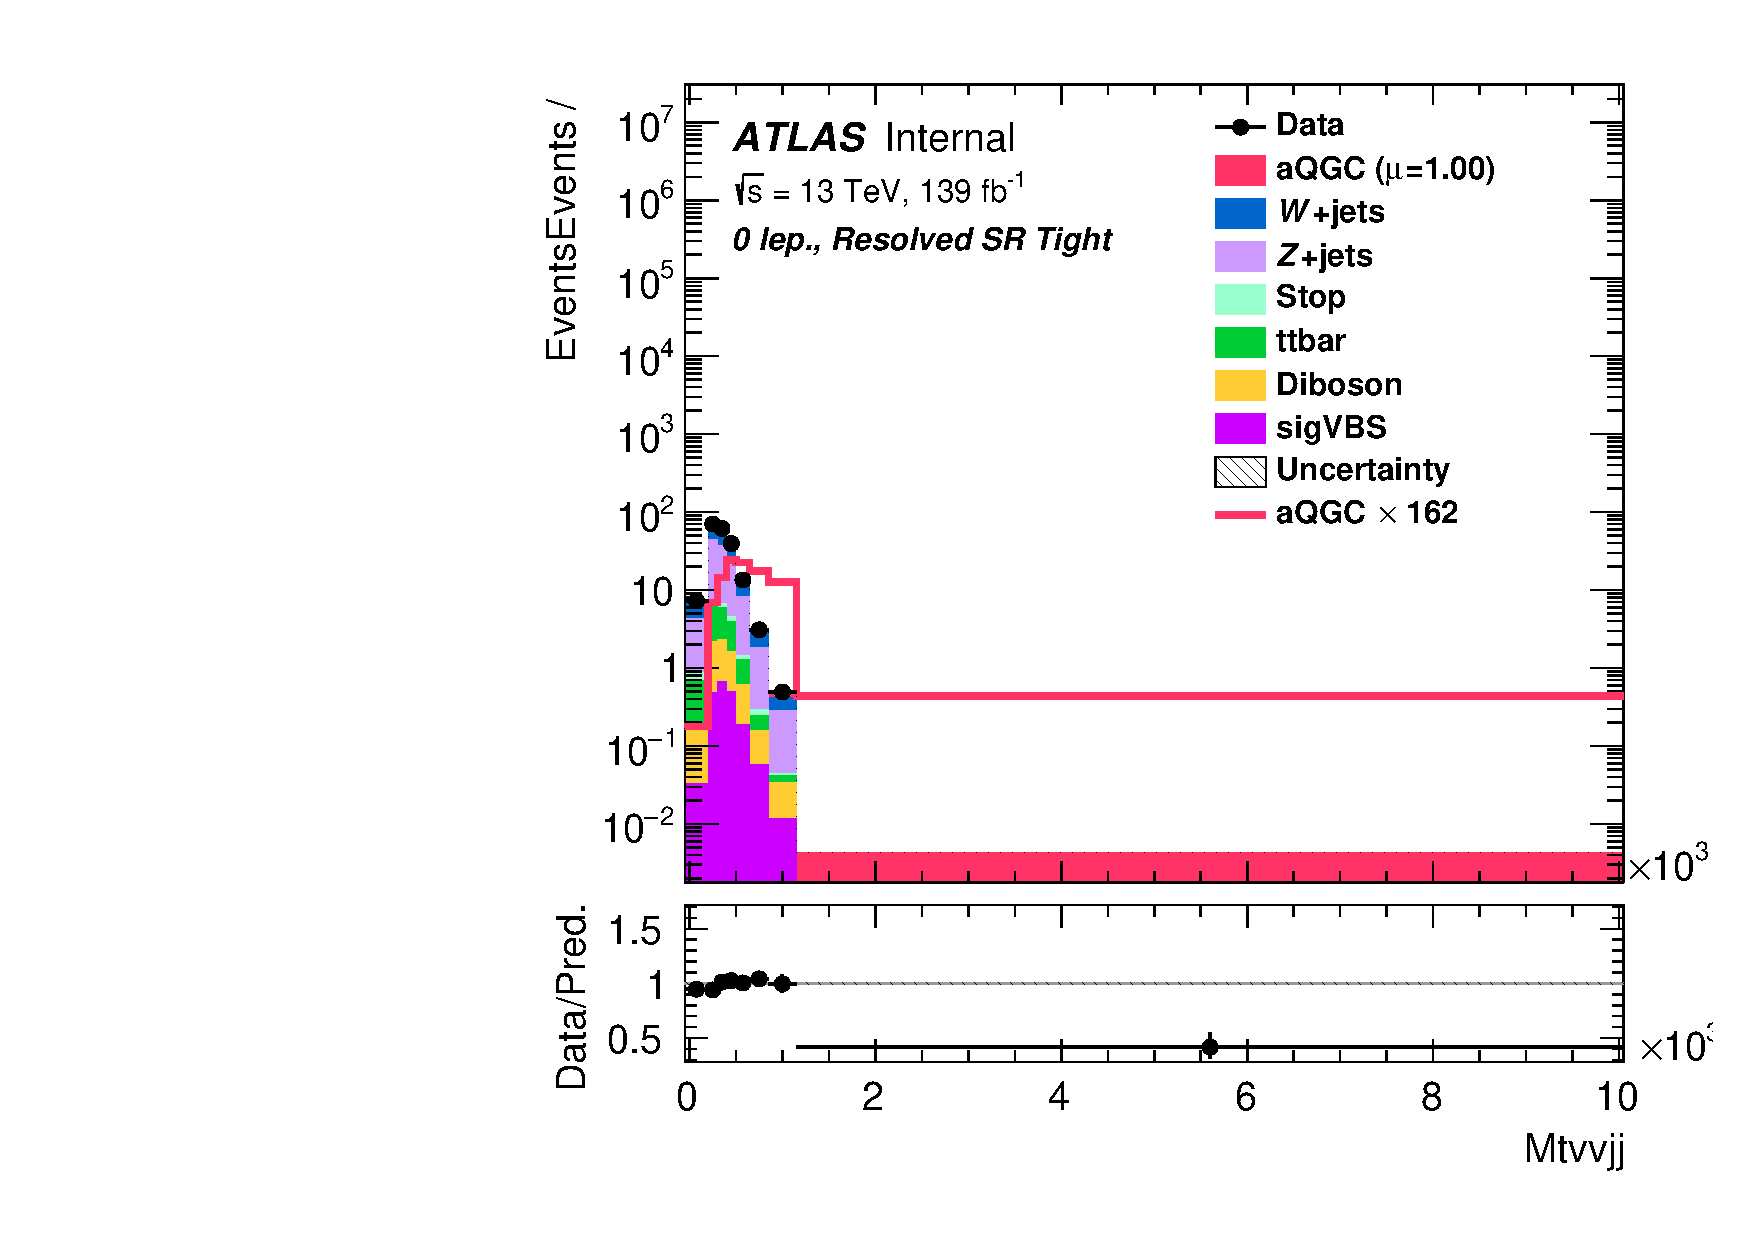
\includegraphics[width=0.32\textwidth]{figures/aQGC/Region_distMtvvjj_DSRVBSFid_BMin0_T0_Y6051_incTag1_J2_L0_incJet1_Prefitlog.pdf}}
%        \caption{Prefit plots for operator FT0 in \tlep channel are shown. The standard model EW signal is floated as the background.}
%        \label{fig:2lepFT0}
%\end{figure}
%
\subsection{Further study to finalize aQGC search strategy}
\label{subsec:2binapproach}

To confirm the result in Section~\ref{subsec:binnedsig} with more realistic setting,
we compared the results with the following conditions.
\begin{itemize}
  \item A fit to $m_{VV}$ distribution as discriminant, without any cuts on the RNN score;
  \item A fit to the RNN score distributions after
        SRs are further separated into two subcategories: \\
        Low $m_{VV}$ : $m_{VV}$ $< 2000$~GeV and \\
        High $m_{VV}$ : $m_{VV}$ $\geq 2000$~GeV. \\
\end{itemize}
With the second option, the number of SRs are twiced as shown in Figure~\ref{fig:2lepTwoBin}.
%(binning??)
Unconditional asimov fit by using FT0 signal in only \tlep channel is performed.
Still only quadratic term is used in this study.
The systematics is not included in the fitting here, just the floated normalization factor is considered.
The asimov data used here is constructed from the background plus SM electroweak $VVjj$ samples.
The expected limits and uncertainty of the expected signal strength of FT0 signal are shown in table~\ref{tab:2binlimit}.
%Significantly better upper limit on the signal strength is obtained by the second option (a fit to RNN score with the categorization by $m_{VV}$)
%than the first option (a fit to $m_{VV}$ distribution).
The signal strength obtained by the second option (a fit to RNN score with the categorization by $m_{VV}$) and the first option (a fit to $m_{VV}$ distribution) is same. 
We found the first option cannot give any constraints on the SM electroweak $VVjj$ signal.
It can be a motivation to use the RNN score also in the aQGC search study.

\begin{figure}[ht]
    \centering
    	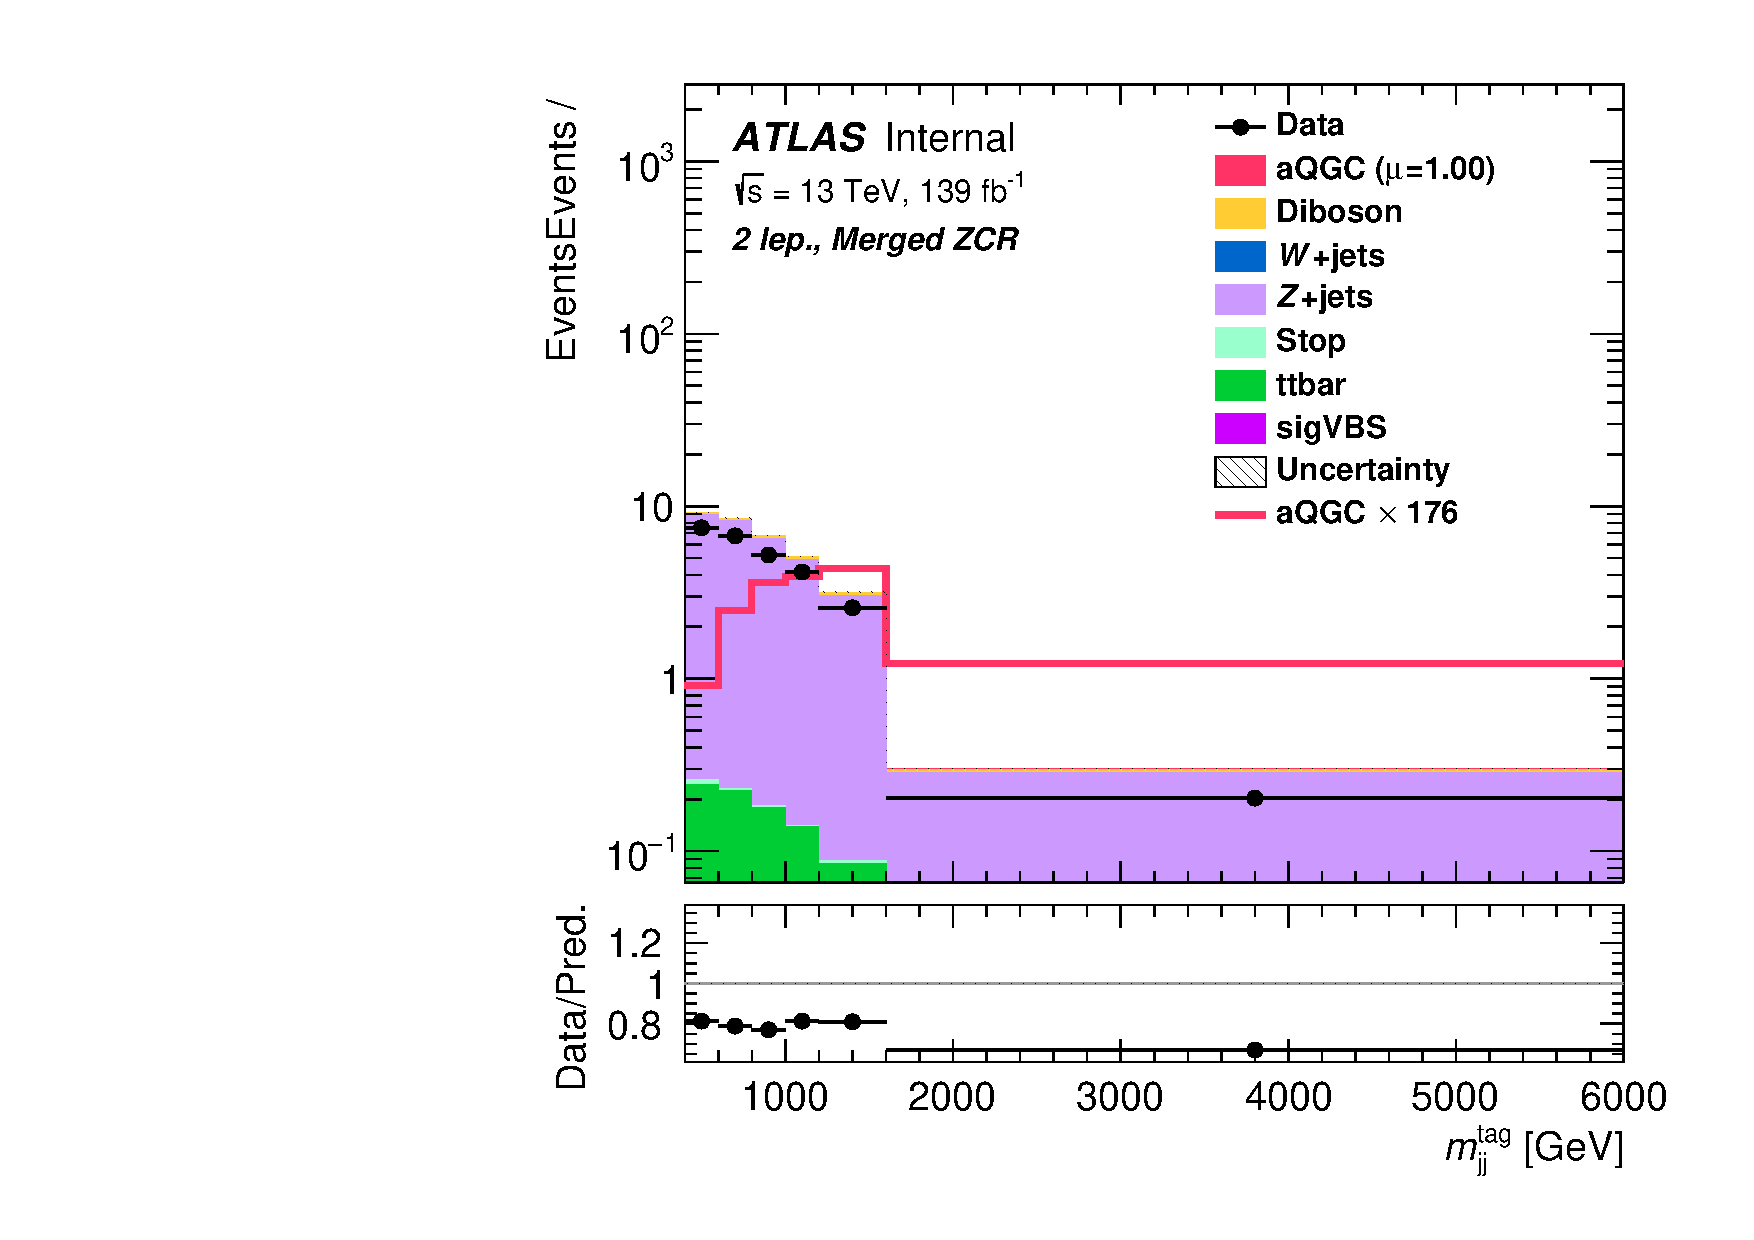
\includegraphics[width=0.32\textwidth]{figures/aQGC/Region_distMTagMerJets_DCRVjet_BMin0_J0_incJet1_L2_T0_incFat1_Y6051_incTag1_Fat1_Prefitlog.pdf}
    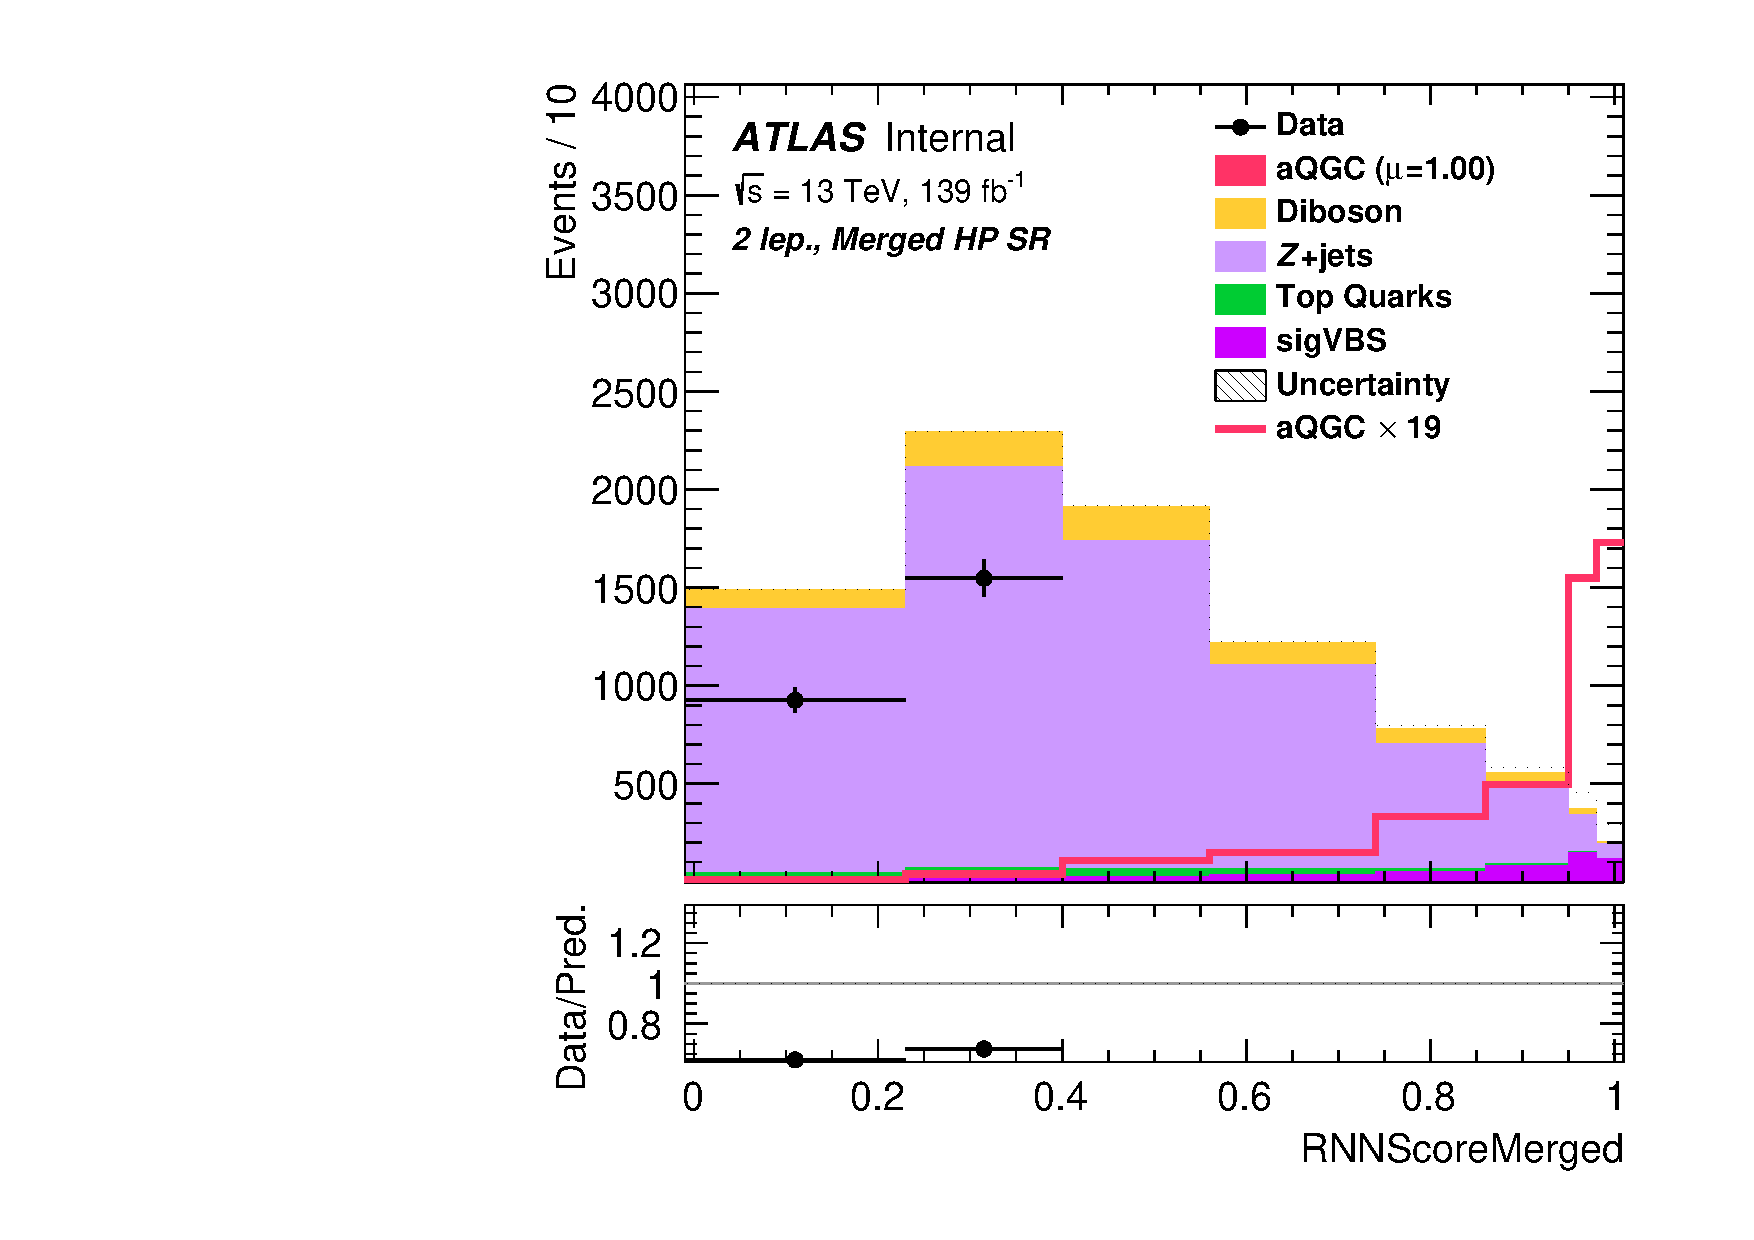
\includegraphics[width=0.32\textwidth]{figures/aQGC/Region_distRNNScoreMerged_DSRVBSHPLMVV_BMin0_J0_incJet1_L2_T0_incFat1_Y6051_incTag1_Fat1_Prefit.pdf}
 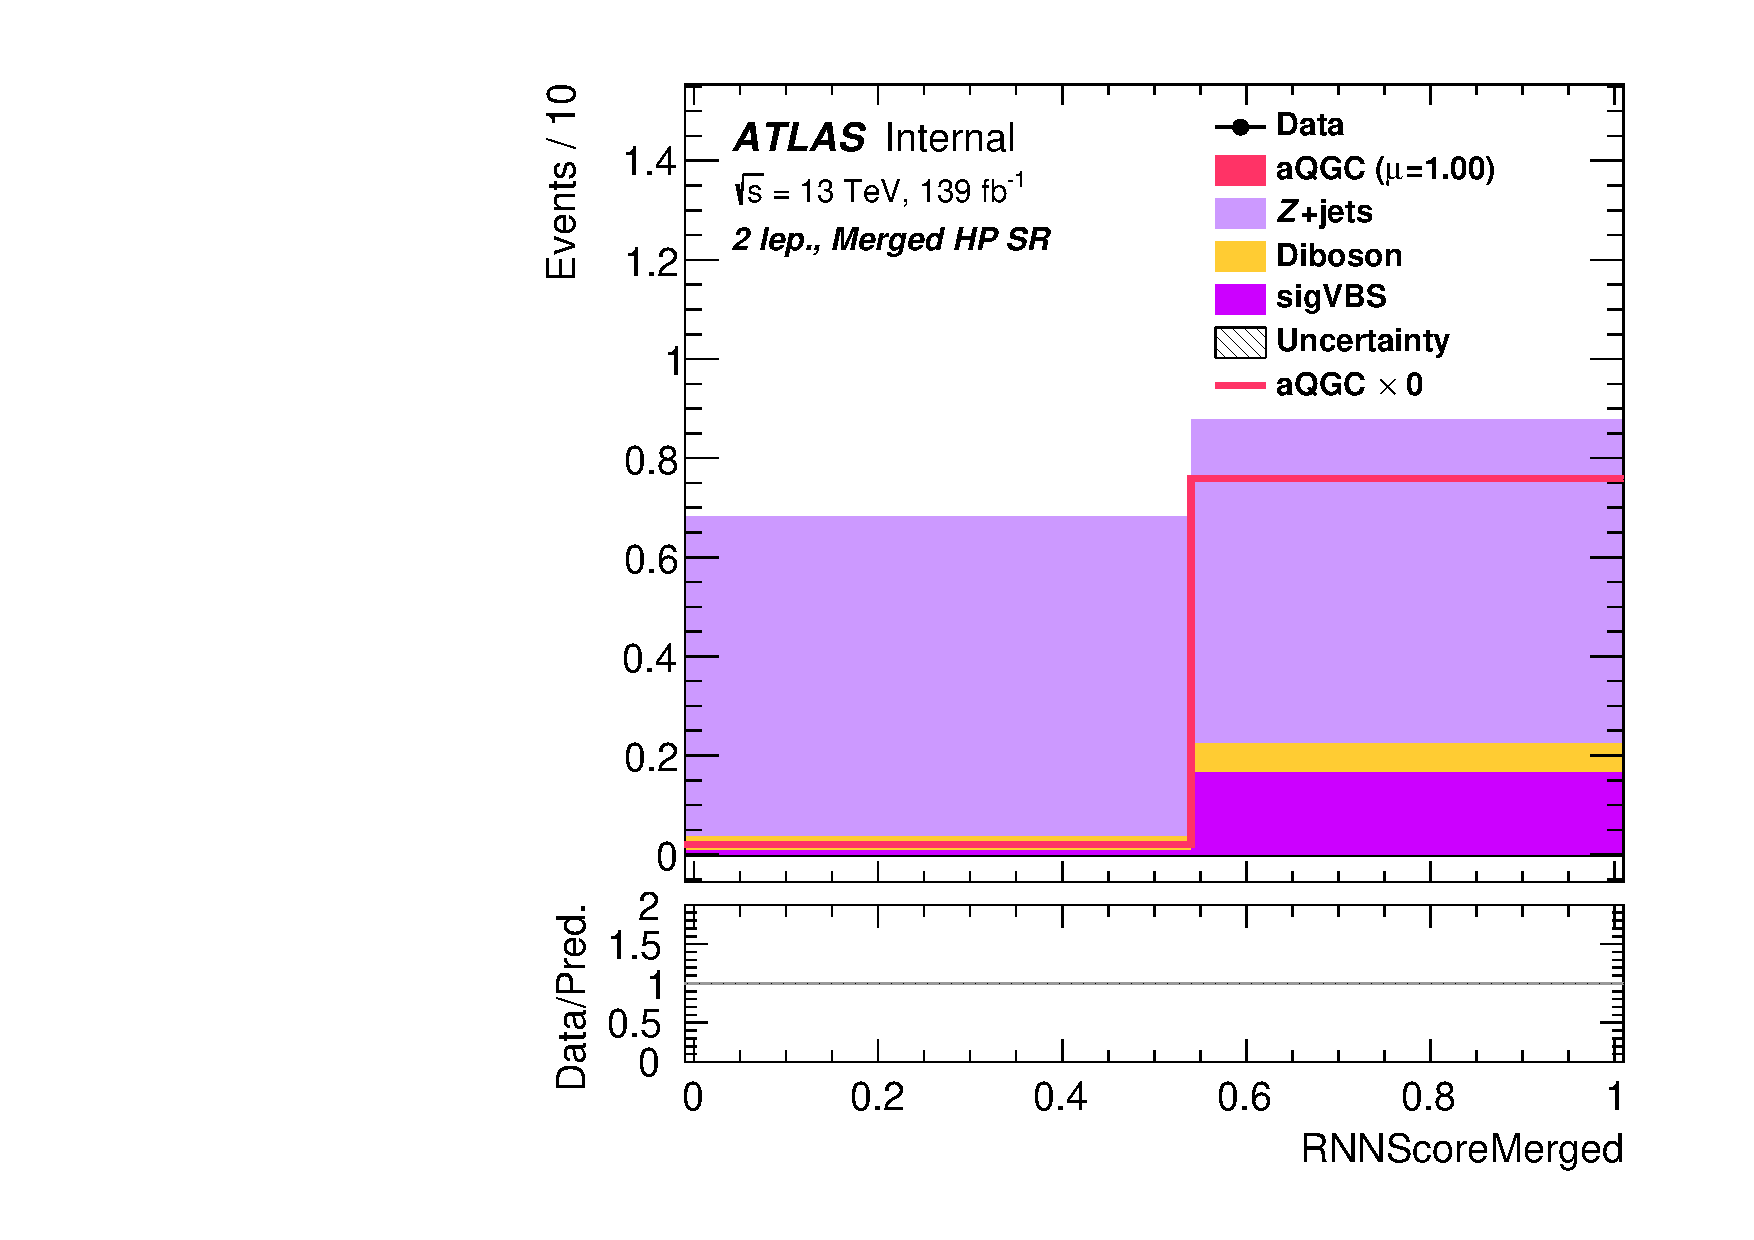
\includegraphics[width=0.32\textwidth]{figures/aQGC/Region_distRNNScoreMerged_DSRVBSHPHMVV_BMin0_J0_incJet1_L2_T0_incFat1_Y6051_incTag1_Fat1_Prefit.pdf}
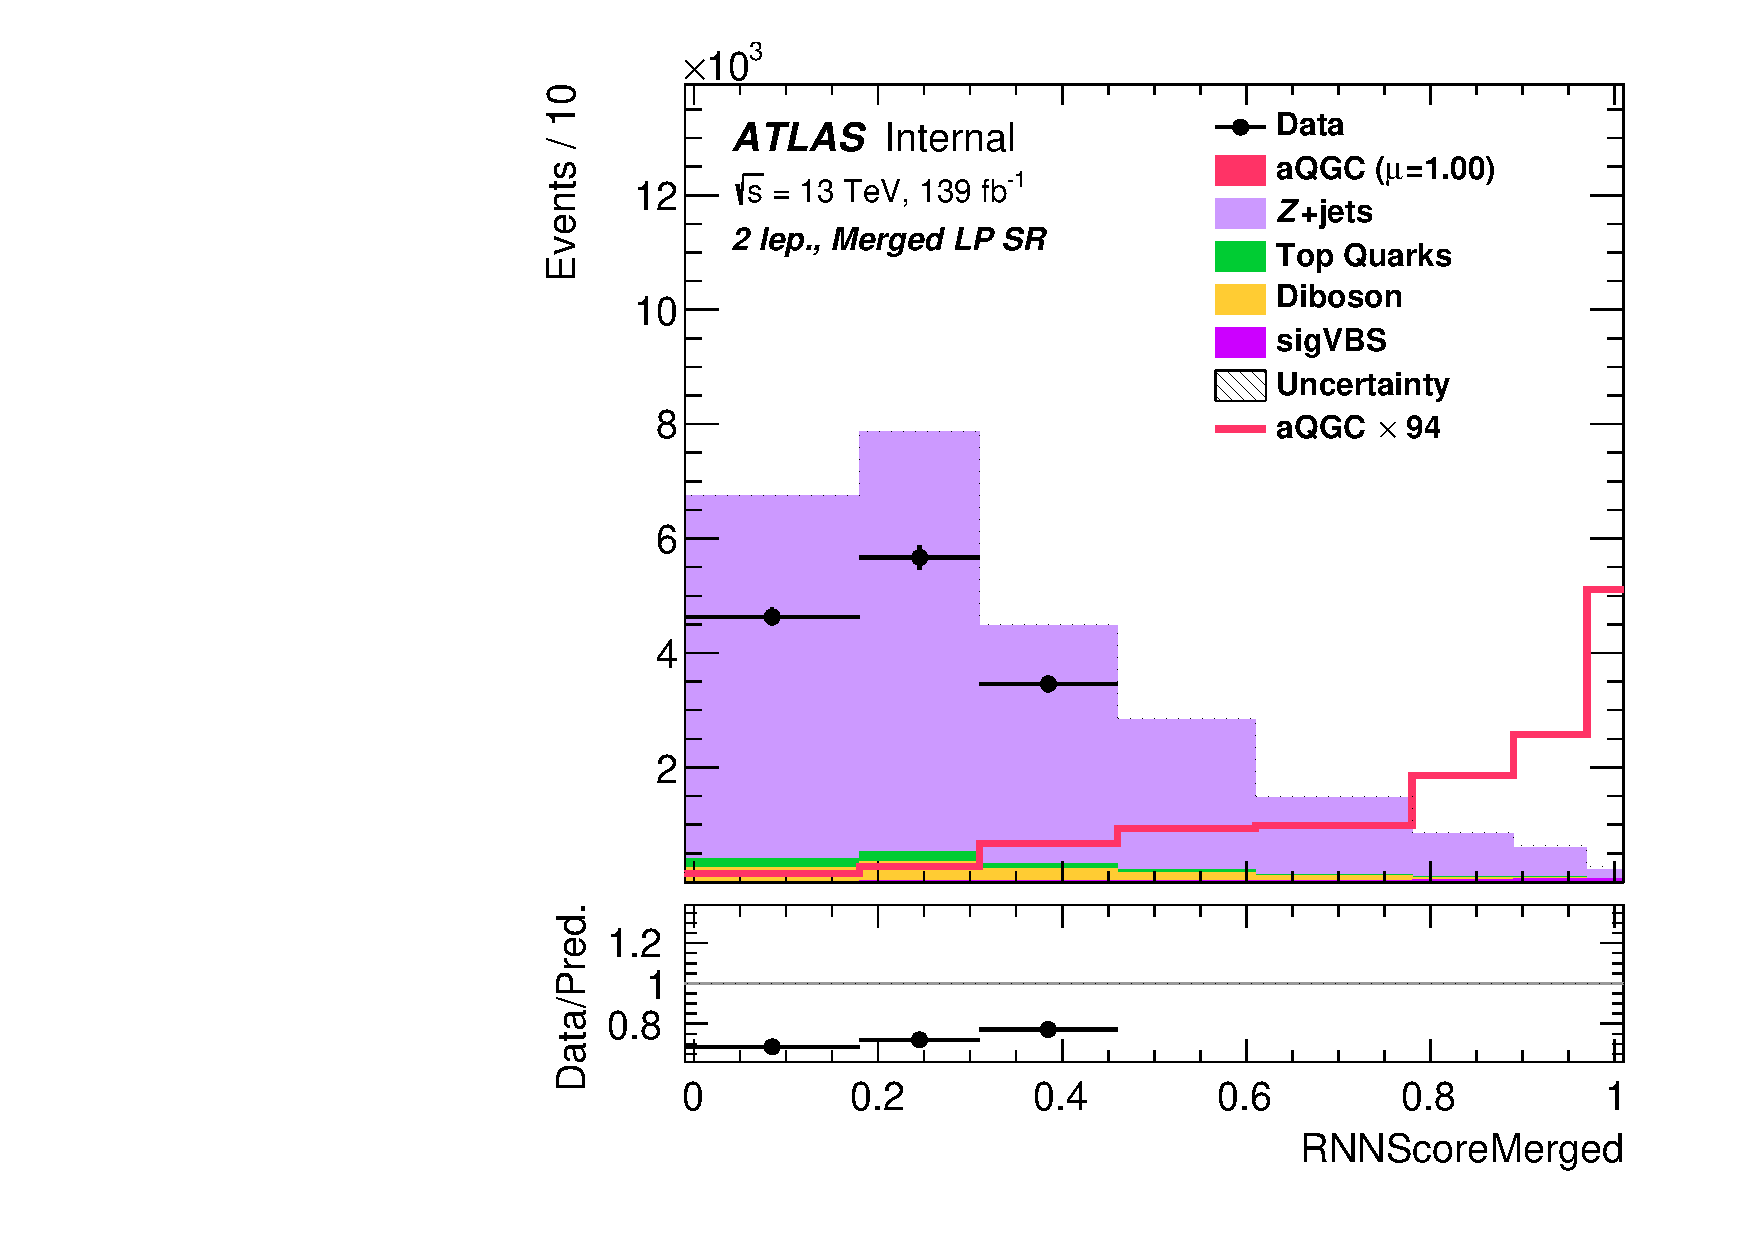
\includegraphics[width=0.32\textwidth]{figures/aQGC/Region_distRNNScoreMerged_DSRVBSLPLMVV_BMin0_J0_incJet1_L2_T0_incFat1_Y6051_incTag1_Fat1_Prefit.pdf}
    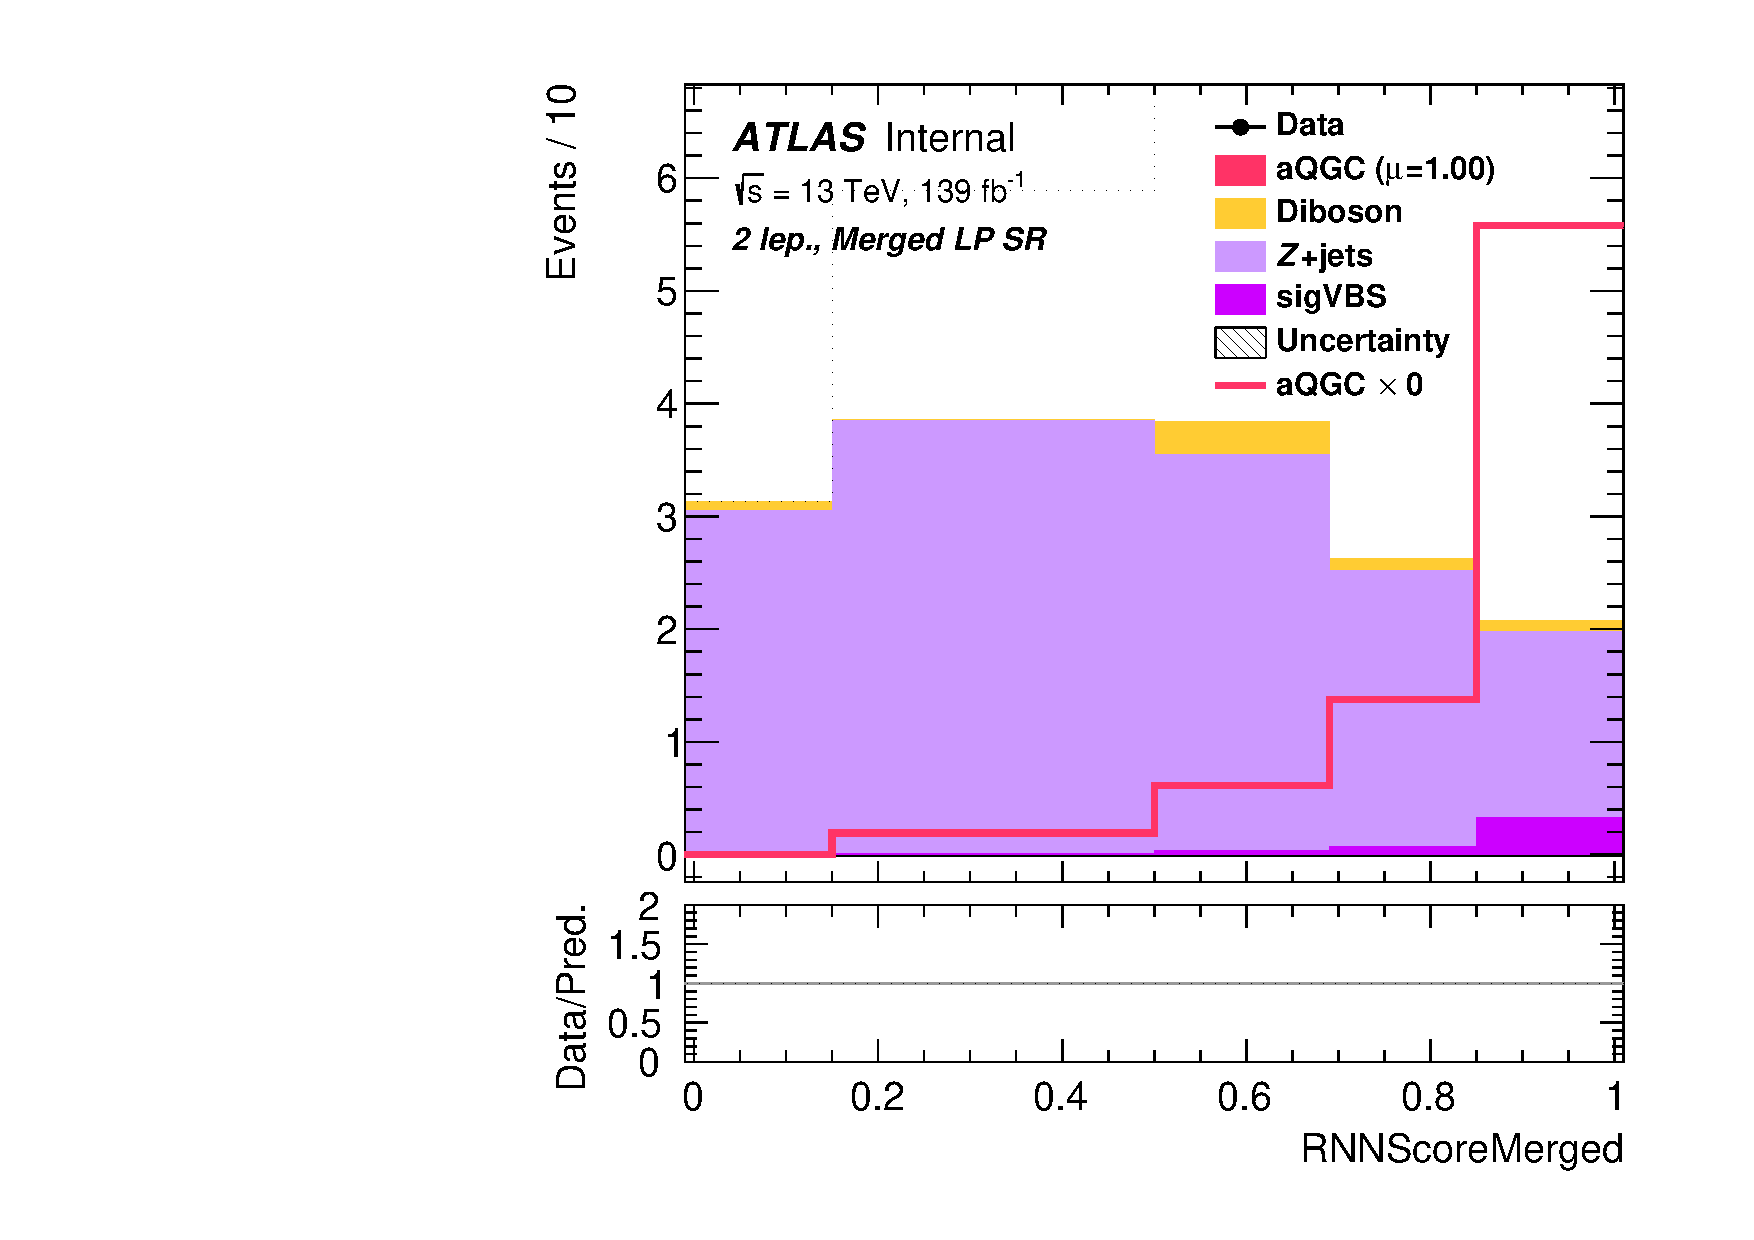
\includegraphics[width=0.32\textwidth]{figures/aQGC/Region_distRNNScoreMerged_DSRVBSLPHMVV_BMin0_J0_incJet1_L2_T0_incFat1_Y6051_incTag1_Fat1_Prefit.pdf}
        \caption{Prefit plots for 2-bin strategy is shown. The RNN score is used as discriminant for signal regions. operator FT0 in \tlep channel are shown. The standard model EW signal is floated as the background.}
        \label{fig:2lepTwoBin}
\end{figure}

%\begin{table}[ht!]
%\small
%\begin{center}
%\resizebox{0.9\textwidth}{!}{
%\begin{tabular}{ | l || l | l | l |}
%\hline
%                                    & Fit to $m_{VV}$ w/o further categorization & Fit to RNN score w/o further categorization  & Fit to RNN scores in separated bins of low- and high-$m_{VV}$  \tabularnewline \hline
%Unconditional fitted $\mu$          & -2.7e-06 $\pm$ 0.067   & 3.38e-05 $\pm0.038$      & 3.35e-05 $\pm0.029$  \tabularnewline \hline
%Norm sigVBS                         & 1 $\pm$ 2.1            & 1 $\pm$ 0.94             & 1 $\pm$ 0.48         \tabularnewline \hline
%Norm Z                              & 1 $\pm$ 0.036          & 1 $\pm$ 0.029            & 1 $\pm$ 0.027        \tabularnewline \hline
%Norm VV                             & 1 $\pm$ 1.13           & 1 $\pm$ 0.71             & 0.99 $\pm$ 0.64      \tabularnewline \hline
%Expected limit of $\mu$             & 0.19                   & 0.72                     & 0.10                 \tabularnewline \hline
%Expected limit of wilson coefficient & 0.44                   & 0.85                     & 0.32                 \tabularnewline \hline
%\end{tabular}
%}
%\caption{Expected signal strength and limits in each two options. only \tlep channel is used for the fit. The result for single bin fit with RNN is also shown as a reference. The normarizations fitted for standard model signal, and Z and diboson backgrounds are shown as Norm in the table.}
%\label{tab:2binlimit}
%\end{center}
%\end{table}

\begin{table}[ht!]
\small
\begin{center}
\resizebox{\textwidth}{!}{
\begin{tabular}{ | l || l | l | l |}
\hline
                                    & Fit to $m_{VV}$ w/o further categorization & Fit to RNN score w/o further categorization  & Fit to RNN scores in separated bins of low- and high-$m_{VV}$  \tabularnewline \hline
Unconditional fitted $\mu$          & 8.83e-06 $\pm0.032$    & 1.02e-04 $\pm0.34$       & 1.09e-05 $\pm0.028$  \tabularnewline \hline
Norm sigVBS                         & 1 $\pm$ 1.08           & 1 $\pm$ 0.79             & 1 $\pm$ 0.41         \tabularnewline \hline
Norm Z                              & 1 $\pm$ 0.012          & 1 $\pm$ 0.010            & 1 $\pm$ 0.01         \tabularnewline \hline
Expected limit of $\mu$             & 0.11                   & 0.70                     & 0.11                 \tabularnewline \hline
Expected limit of wilson coefficient & 0.33                  & 0.84                     & 0.33                 \tabularnewline \hline
\end{tabular}
}
\caption{Expected signal strength and limits in each two options. only \tlep channel is used for the fit. The result for single bin fit with RNN is also shown as a reference. The normarizations fitted for standard model signal, and Z backgrounds are shown as Norm in the table.}
\label{tab:2binlimit}
\end{center}
\end{table}

%\subsection{Optimization of the threshold of 2-bin approach}
%\label{subsec:aQGCbinninb}
Of course, the optimal threshold of $m_{VV}$ can be different depending on the clipping energy.
In addition, a fine tuning of the $m_{VV}$ threshold might be needed by considering the stability of the background stimation.
The expected limit is shown in each threshold for $m_{VV}$ of 1000~GeV, 1500~GeV, 2000~GeV for variety of the clipping points in Figure~\ref{fig:ThresholdScan}.
As expected, higher $m_{VV}$ threshold is preferred at the higher clipping point, while lower $m_{VV}$ threshold is favored at the lower clipping point.
1500~GeV is chosen as the best compromize to separate SRs into low- and high-$m_{VV}$ bins.

Since the meaning of the actual $m_{VV}$ distributions used in each letpon channel are different
(fully reconstructed system in \tlep and in \olep (solving neutrino ambiguity) and transverse mass in \zlep)
the optimal thresholds to separate SRs into low- and high-$m_{VV}$ bins in \olep\ and \zlep\ channels 
are determined as follows.
In \olep\ channel, the same threshold as \tlep\ channel, 1500~GeV, is just chosen since the reconstructed $m_{VV}$ distribution is similar. 
%(?)
In \zlep channel the threshold needs to be optimized, since it uses \mt\ instead of $m_{VV}$.
As shown in Figure~\ref{fig:mVVdist} the \mt\ shape in \zlep\ channel is different from $m_{VV}$ in \tlep channel.
Here, the background yield in each bin of the high-$\mt$ regions is adjusted to be more than 5 so that
the asymptotic calculation of the sensitivity is ensured with the certain number of background events.
The threshold finalized is shown in Table, for each lepton channels and for each regions.

Only in \tlep\ channel,
less than 5 background events are expected in the second bin of the HP signal region.
%We are going to test if the asymptotic fomulae works fine, by running toy experiments [TO DO].
%
\begin{figure}[h]
        \centering
    	\includegraphics[width=0.50\textwidth]{figures/aQGC/ClippedFT02bin.pdf}
        \caption{Expected limits for 5 clipping points with each threshold for dividing $m_{VV}$ into 2 bins.}
        \label{fig:ThresholdScan}
\end{figure}

\begin{figure}[ht]
    \centering
    	\includegraphics[width=0.32\textwidth]{figures/aQGC/MVV/Region_distMllJ_DSRVBSHP_BMin0_J0_incJet1_L2_T0_incFat1_Y6051_incTag1_Fat1_Prefitlog.pdf}
    \includegraphics[width=0.32\textwidth]{figures/aQGC/MVV/Region_distMllJ_DSRVBSLP_BMin0_J0_incJet1_L2_T0_incFat1_Y6051_incTag1_Fat1_Prefitlog.pdf}
  \includegraphics[width=0.32\textwidth]{figures/aQGC/MVV/Region_distMlljj_DSRVBSFid_BMin0_T0_Y6051_incTag1_J2_L2_incJet1_Prefitlog.pdf}
    	%\subfigure[ 1lep HP SR ]{\includegraphics[width=0.32\textwidth]{figures/aQGC/MVV/}}
    	%\subfigure[ 1lep LP SR ]{\includegraphics[width=0.32\textwidth]{figures/aQGC/MVV/}}
    	%\subfigure[ 1lep Fid SR ]{\includegraphics[width=0.32\textwidth]{figures/aQGC/MVV/}}
    	\includegraphics[width=0.32\textwidth]{figures/aQGC/MVV/Region_distMtvvJ_DSRVBSHP_BMin0_J0_incJet1_L0_T0_incFat1_Y6051_incTag1_Fat1_Prefitlog.pdf}
    \includegraphics[width=0.32\textwidth]{figures/aQGC/MVV/Region_distMtvvJ_DSRVBSLP_BMin0_J0_incJet1_L0_T0_incFat1_Y6051_incTag1_Fat1_Prefitlog.pdf}
 \includegraphics[width=0.32\textwidth]{figures/aQGC/MVV/Region_distMtvvjj_DSRVBSFid_BMin0_T0_Y6051_incTag1_J2_L0_incJet1_Prefitlog.pdf}
        \caption{fig:$m_{VV}$ distribution for \tlep (left) and Mtv distribution for \zlep (right)}
        \label{fig:mVVdist}
\end{figure}

\begin{table}[ht!]
\small
\begin{center}
%\resizebox{0.9\textwidth}{!}{
\begin{tabular}{ | l || l | l | l |}
\hline
Threshold values (GeV)          & SRVBS\_HP  & SRVBS\_LP & SRVBS\_Fid  \tabularnewline \hline
0-lepton & 1050      & 1200     & 1200       \tabularnewline \hline
1-lepton & 1500      & 1500     & 1500       \tabularnewline \hline
2-lepton & 1500      & 1500     & 1500       \tabularnewline \hline
\end{tabular}
\caption{Threshold values}
\label{tab:2binthreshold}
\end{center}
\end{table}



\subsection{Statistical treatment to obtain limits}


\subsection{Expected limits}
Finally, by using both quadratic and interference terms as a combined signal template,
the expected 95\% CL upper and lower limits are obtained by the fit to the asimov dataset constructed
from the background plus SM $VVjj$ samples.
The POI is set to include both QUAD terms and INT terms simultaneously, thereby two signal strength is parametrized as $\mu_{QUAD} = \mu_{INT}^2$.
All SRs in \zlep, \olep\ and \tlep channels are separated into low- and high-$m_{VV}$ bins as discussed in Section~\ref{subsec:2binapproach}
and combined statistically.
All systematics uncertainties discussed for Standard Model measurement is included in the fitting.
Due to the small statistics in high-$m_{VV}$ regions compared with the low-$m_{VV}$ regions,
the overall behaviors of the post-fit nuisance parameters are almost the same as the SM measurement.
The result is shown in Figure~\ref{fig:aQGClimits}.
The limits are shown at 5 clipping energy points of [1.5, 2.0, 3.0, 5.0, $\infty$]~TeV.
The unitarity bound from the theoretical calclation \cite{PhysRevD.101.113003} is overlaid.
The upper and lower limits correspond to the signal hypotheses showing $\Delta NLL \sim \frac{1}{2}\chi^2 = 1.0$.
Table~\ref{tab:aQGClimits} shows the uniterized and ununiterized expected limits from figure~\ref{fig:aQGClimits}.

\begin{figure}[ht]
    \centering
    \includegraphics[width=0.40\textwidth]{figures/aQGC/ClippedFT0CI.pdf}
    	\includegraphics[width=0.40\textwidth]{figures/aQGC/ClippedFM0CI.pdf}
    	\includegraphics[width=0.40\textwidth]{figures/aQGC/ClippedFS02CI.pdf}
        \caption{Expected limits for 5 clipping points are shown for each Wilson coefficient FT0 (left), FM0 (right), FS02 (middle).}
        \label{fig:aQGClimits}
\end{figure}

%\begin{table}[ht!]
%\small
%\begin{center}
%%\resizebox{0.9\textwidth}{!}{
%\begin{tabular}{ | l || l | l | l | l | l |}
%\hline
%                   & 1.5 [ TeV ] & 2.0 [ TeV ] & 3.0 [ TeV ] & 5.0 [ TeV ] & $\infty$                  \tabularnewline \hline
%FT0                & [ -1.02, 0.88 ]  & [ -0.47, 0.41 ]  & [ -0.25, 0.21 ]  & [ -0.16, 0.15 ]  & [ -0.16, 0.16 ]              \tabularnewline \hline
%FM0                & [ -5.63, 5.62 ]  & [ -2.47, 2.47 ]  & [ -1.37, 1.37 ]  & [ -1.08, 1.09 ]  & [ -1.06, 1.07 ]              \tabularnewline \hline
%FS02               & [ -11.06, 11.07 ]  & [ -5.60, 5.64 ]  & [ -3.63, 3.68 ]  & [ -3.27, 3.32 ]  & [ -3.27, 3.32 ]              \tabularnewline \hline
%\end{tabular}
%\caption{Expected limits for each clipping point. Ununiterized limit is shown as the limit with no clipping energy, labeled as $\infty$ in figure~\ref{fig:aQGClimits}.}
%\label{tab:aQGClimits}
%\end{center}
%\end{table}

%uniterized limit
\begin{table}[ht!]
\small
\begin{center}
%\resizebox{0.9\textwidth}{!}{
\begin{tabular}{ | l || l | l |}
\hline
Wilson coefficient & uniterized expected limit  & ununiterized expected limit \tabularnewline \hline
FT0                &  [ -0.48, 0.39 ]            & [ -0.16, 0.16 ]              \tabularnewline \hline
FM0                &  [ -2.99, 2.97 ]            & [ -1.06, 1.07 ]              \tabularnewline \hline
FS02               &  [ -5.46, 5.61 ]            & [ -3.27, 3.32 ]              \tabularnewline \hline
\end{tabular}
\caption{Uniterized and ununiterized expected limits. Uniterized limit is the intersection point of the thoretical unitality bound and experimental limit line. Ununiterized limit is the limit with no clipping energy, labeled as $\infty$ in figure~\ref{fig:aQGClimits}.}
\label{tab:aQGClimits}
\end{center}
\end{table}

